\documentclass[12pt,letter]{article}
\usepackage{mathptmx} % added for time new roman font
\usepackage[left=1in,right=1in,top=1in,bottom=1in]{geometry}
\usepackage[latin1]{inputenc}


\usepackage{amsmath}




% defines all example enviorment
\usepackage[framemethod=tikz]{mdframed} % added for the box around examples
\newtheorem{ex}{Example}
\numberwithin{ex}{section} % allows for the use of example numbers that lign up with the section numbers
\newenvironment{example}{\begin{mdframed}[middlelinewidth=0.5mm]\begin{ex}\normalfont}{\end{ex}\end{mdframed}}

% defines the quotation enviorment 
\usepackage{xcolor}
\newcommand{\quotebox}[2]{\begin{center}\fcolorbox{white}{blue!15!gray!15}{\begin{minipage}{0.9\linewidth}\vspace{10pt}\center\begin{minipage}{0.8\linewidth}{\space\Huge``}{#1}{\Huge''}{\break\null\hfill} {\small #2}  \end{minipage}\medbreak\end{minipage}}\end{center}}


\usepackage{amsfonts}
\usepackage{amssymb}
\usepackage{graphicx}
\usepackage{float}
\usepackage{booktabs}
\usepackage{parskip} % remove all the paragraph indents


\usepackage{setspace}
\usepackage[colorlinks=true]{hyperref}
\usepackage{textcomp} 
\usepackage{multicol} 

\usepackage{mathtools}          %loads amsmath as well added for the piece wise function
\DeclarePairedDelimiter\Floor\lfloor\rfloor
\DeclarePairedDelimiter\Ceil\lceil\rceil

 
\newcounter{NumberInTable}
\newcommand{\LTNUM}{\stepcounter{NumberInTable}{(\theNumberInTable)}}

\newcommand{\Laplace}[1]{\ensuremath{\mathcal{L}{\left[#1\right]}}}
\newcommand{\InvLap}[1]{\ensuremath{\mathcal{L}^{-1}{\left[#1\right]}}}
\renewcommand{\textuparrow}{$\uparrow$}

\begin{document}

		\section{Forced Vibrations}

	
		\subsection{Harmonic excitations of undamped systems}

			Consider the system
			\begin{figure}[H]
				\centering
				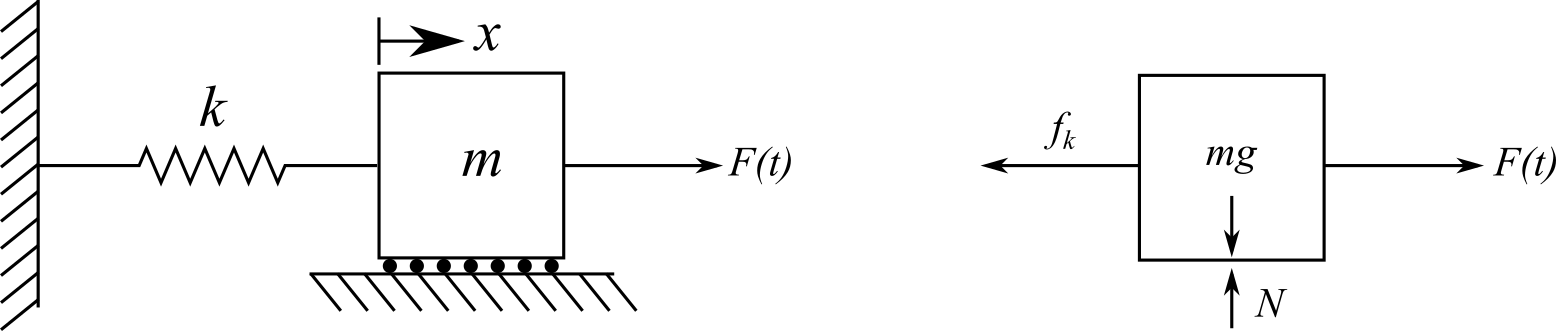
\includegraphics[width=0.7\textwidth]{../Figures/forced_spring_mass_system_with_FBD.png}
			\end{figure}	
			For simplicity, let us consider a harmonic excitation for $F(t)$ such that:
			\begin{equation}
				F(t) = F_0\text{cos}(\omega t)
			\end{equation}							
			note that here, $\omega$ has no subscript and is the frequency in rad/sec of the driving force. $F_0$ represents the magnitude of the applied force. This is often called the \textbf{input frequency, driving frequency, or forcing frequency}. Summing the forces in the above figure in the $x$ direction yields:
			\begin{equation}
				m \ddot{x}(t)+kx(t) = F_0\text{cos}(\omega t)
			\end{equation}			
			For convinces we can convert this to the standard form:					
			\begin{equation}
				\ddot{x}(t)+\omega_n^2x(t) = f_0\text{cos}(\omega t)
			\end{equation}					
			where:
			\begin{equation}
				f_0 = \frac{F_0}{m}
			\end{equation}	
			Again, this is a linear, nonhomogeneous, O.D.E. that we need to solve. It is nonhomogeneous because there are no terms related to $x$ on the right-hand side of the equation. One way to solve such an equation to recall that the solution for a nonhomogeneous equation is the sum of the homogeneous and particular solutions. 
			\begin{equation}
				x(t) = x_h(t) + x_p(t)
			\end{equation}	
			First, knowing that the solution is the sum of two parts, vibration caused by the forcing function and the oscillations caused by the system of springs and masses, we set the equation for the homogeneous solution to be:
			\begin{equation}
				x_h(t) = A\text{sin}(\omega_n t + \phi)
			\end{equation}			
			Next, we will denote the particular solution as $x_p$. $x_p$ can be determined by observing the systems and assuming that it is in form of the forcing function, therefore:
			\begin{equation}
				f_0\text{cos}(\omega t)
			\end{equation}	
			becomes:
			\begin{equation}
				x_p = x_p(t) =X\text{cos}(\omega t)
			\end{equation}						
			where, $x_p$ is the particular solution and $X$ is the amplitude of the forced response. Our total solution now becomes:
			\begin{equation}
				x(t) = A\text{sin}(\omega_n t + \phi) + X\text{cos}(\omega t) 
			\end{equation}				
			This approach, of assuming that $x_p=X\text{cos}(\omega t)$, in order to determine the particular solution is called the \textbf{method of undetermined coefficients}. To calculate $X$, first we take the equations for $x_p(t)$ and $\ddot{x}_p(t) $:
			\begin{equation}
				x_p(t) = X\text{cos}(\omega t)
			\end{equation}	
			\begin{equation}
				\ddot{x_p}(t) = -\omega^2X\text{cos}(\omega t)
			\end{equation}				
			and substituting these into the equation of motion in standard from yields:
			\begin{equation}
				-\omega^2X\text{cos}(\omega t)+\omega_n^2X\text{cos}(\omega t) = f_0\text{cos}(\omega t)
			\end{equation}		
			As long as 	$\text{cos}(\omega t) \neq  0$, solving for X yields:
			\begin{equation}
				X = \frac{f_0}{\omega_n^2-\omega^2}
			\end{equation}		
			Therefore, as long as $\omega_n \neq \omega$, the particular solution can take the form
			\begin{equation}
				x_p = \frac{f_0}{\omega_n^2-\omega^2}\text{cos}(\omega t)
			\end{equation}						
			This then expands to the total form
			\begin{equation}
				x(t) = A\text{sin}(\omega_n t + \phi) + \frac{f_0}{\omega_n^2-\omega^2}\text{cos}(\omega t)
			\end{equation}				
			expanding this to the general form for the homogeneous solution obtains the equation
			\begin{equation}
				x(t) = A_1\text{sin}(\omega_n t) + A_2\text{cos}(\omega_n t) + \frac{f_0}{\omega_n^2-\omega^2}\text{cos}(\omega t)
			\end{equation}				
			As before, we need to determine the values for the coefficients $A_1$ and $A_2$ by enforcing the initial conditions $x_0$ and $v_0$. Setting the time to zero ($t=0$) and solving the initial displacement leads to:
			\begin{equation}
				x(0) = x_0 = A_2 + \frac{f_0}{\omega_n^2-\omega^2}
			\end{equation}				
			or:
			\begin{equation}
				A_2 = x_0-\frac{f_0}{\omega_n^2-\omega^2}
			\end{equation}	
			again, solving the equation in terms of velocity:
			\begin{equation}
				\dot{x}(t) = A_1\omega_n\text{cos}(\omega_n t) - A_2 \omega_n \text{sin}(\omega_n t) - \omega \frac{f_0}{\omega_n^2-\omega^2}\text{sin}(\omega t)
			\end{equation}	
			and solving for the initial velocity at $t=0$:
			\begin{equation}
				\dot{x}(0) = v_0 =  A_1 \omega_n
			\end{equation}				
			or:
			\begin{equation}
				A_1 = \frac{v_0}{\omega_n}
			\end{equation}				
			Therefore, combining the equations we get:
			\begin{equation}
				x(t) = \Big(\frac{v_0}{\omega_n}\Big)\text{sin}(\omega_n t) + \Big(x_0-\frac{f_0}{\omega_n^2-\omega^2}\Big)\text{cos}(\omega_n t) + \frac{f_0}{\omega_n^2-\omega^2}\text{cos}(\omega t)
			\end{equation}	
			As before, we can relate $A_1$ and $A_2$ to each other through the basic trigonometric identities. This yields, 
			\begin{equation}
				x(t) = A\text{sin}(\omega_n t + \phi) + X\text{cos}(\omega t) 
			\end{equation}				
			\begin{equation}
				A = \sqrt{\bigg(\frac{v_0}{\omega_n}\bigg)^2+(x_0-X)^2}
			\end{equation}				
			\begin{equation}
				\phi = \text{tan}^{-1}\bigg(\frac{\omega_n(x_0-X)}{v_0}\bigg)
			\end{equation}				
			\begin{equation}
				X = \frac{f_0}{\omega_n^2-\omega^2}
			\end{equation}				
			The forced and unforced plots can relate to each other as (Note that the forcing function uses the axis on the right):
			\begin{figure}[H]
				\centering
				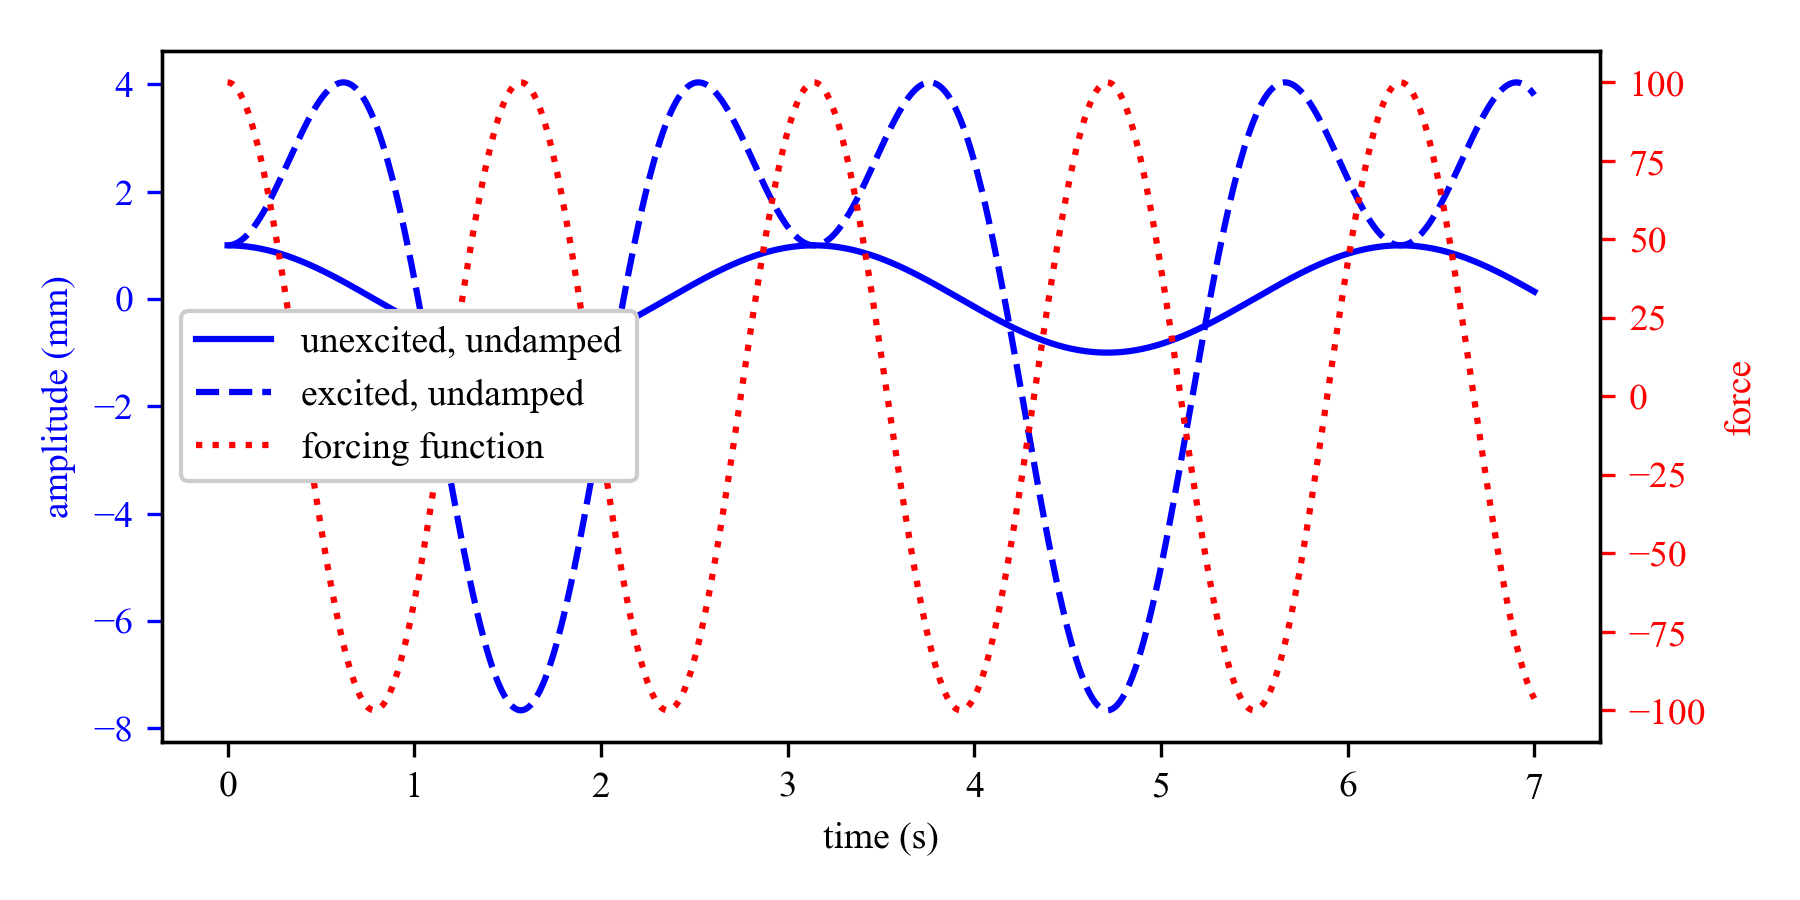
\includegraphics[width=0.9\textwidth]{../Figures/forced_unforced_plot.png}
			\end{figure}	
			for a system with $k$ = 10 N/m, $m$ = 2.5 kg, $\omega$ = 4 rad/sec, $F_0$ = 0.1 kN, $x_0$ = 1 mm, and $v_0$ = 0 mm. 
			
			
		\subsection{Harmonic resonance}			
			
			Recall that our solution from before assumed that $\omega_n \neq \omega$, however, if $\omega_n = \omega$ then the system will develop the phenomenon of resonance. Mathematically, this means the amplitude of the vibrations becomes unbounded. The prior choice of $X\text{cos}(\omega t)$ for the particular solution fails as it is also a solution for a homogeneous equation. Therefore, the particular solution can be written as 
			\begin{equation}
				x_p(t) = t X\text{sin}(\omega t)
			\end{equation}				
			Substituting this into the standard form equation (from Boyce and DiPrima (1997)) and solving for X yields:
			\begin{equation}
				x_p(t) = \frac{f_0}{2 \omega} t \text{sin}(\omega t)
			\end{equation}	
			thus, the total solution can now be written as:
			\begin{equation}
				x(t) = A_1\text{sin}(\omega t) + A_2\text{cos}(\omega t) + \frac{f_0}{2 \omega} t \text{sin}(\omega t)
			\end{equation}			
			Note that $\omega_n=\omega$, therefore, the frequencies are all in terms of the driving frequency $\omega$. Again, evaluating the solution at $t=0$ for the initial conditions $x_0$ and $v_0$ yields:
			\begin{equation}
				x(t) = \Big(\frac{v_0}{\omega}\Big)\text{sin}(\omega t) + x_0\text{cos}(\omega t) + \frac{f_0}{2 \omega} t \text{sin}(\omega t)
			\end{equation}			
			The following plot shows the forced response of a spring-mass system driven harmonically at its natural frequency.
			\begin{figure}[H]
				\centering
				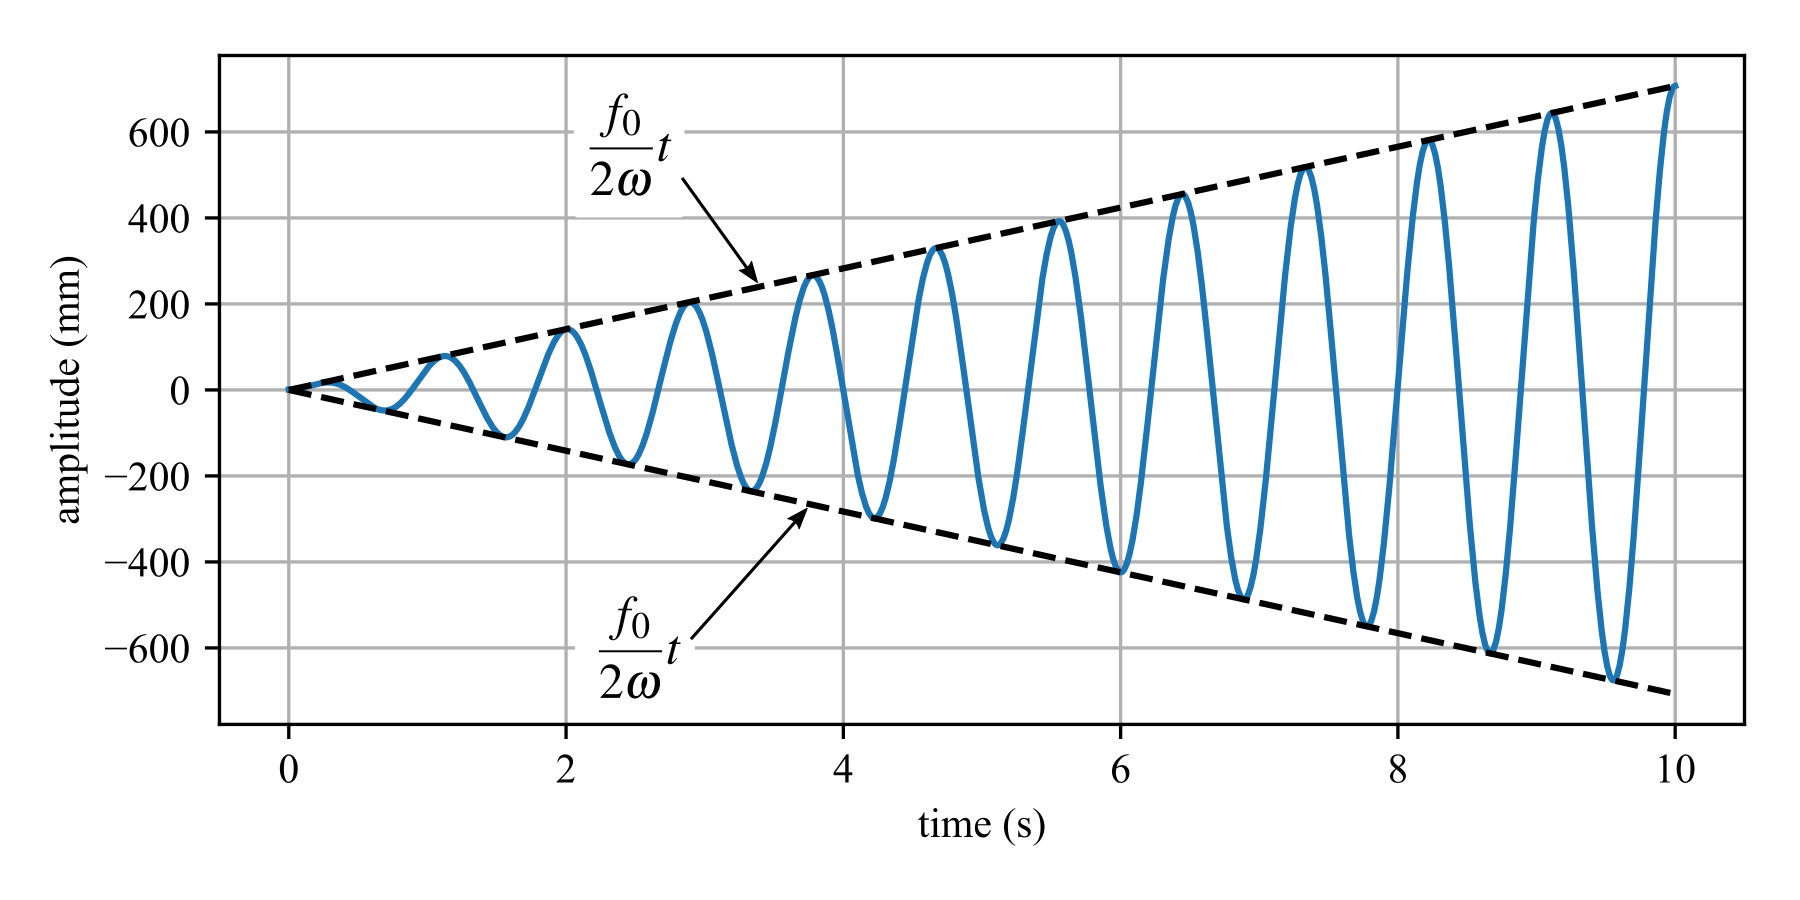
\includegraphics[]{../Figures/resonance.png}
			\end{figure}				

\begin{example}

			Compute solutions for the homogeneous and partial solution separately, than compute the total response of a spring-mass system with the following values: $k$ = 1000 N/m, $m$ = 10 kg, subject to a harmonic force of magnitude $F_0$ = 100 N and frequency of 8.162 rad/s, and initial conditions given by $x_0$ = 0 m and $v_0$ = 0 m/s. Plot the response.
			
			\begin{figure}[H]
				\centering
				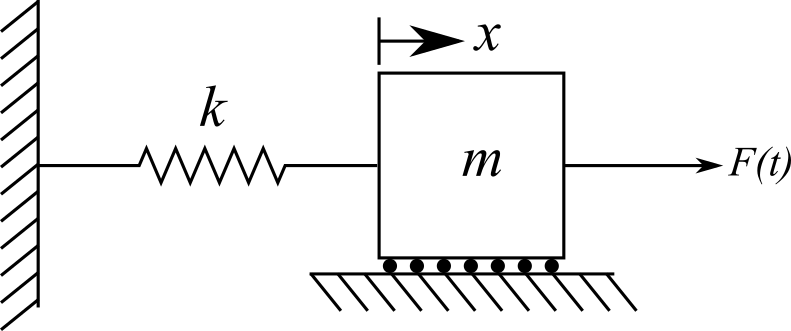
\includegraphics[width=0.5\textwidth]{../Figures/forced_spring_mass_system.png}
			\end{figure}
			
			First, make sure that the system is not in resonance. Calculating that $\omega_n = \sqrt{1000/10} = 10$ shows us that $\omega_n \neq \omega$. Next knowing that $f_0 = F_o/m = 10$ we can find the homogeneous and partial solutions as:
			\begin{equation}
				x_h(t) = A\text{sin}(\omega_n t + \phi)
			\end{equation}				
			\begin{equation}
				x_p(t) = X\text{cos}(\omega t) 
			\end{equation}	
			also:			
			\begin{equation}
				x(t) = x_h(t) + x_p(t)
			\end{equation}	
			where:			
			\begin{equation}
				A = \sqrt{\bigg(\frac{v_0}{\omega_n}\bigg)^2+(x_0-X)^2} = 
			\end{equation}				
			\begin{equation}
				\phi = \text{tan}^{-1}\bigg(\frac{\omega_n(x_0-X)}{v_0}\bigg)
			\end{equation}				
			\begin{equation}
				X = \frac{f_0}{\omega_n^2-\omega^2}
			\end{equation}			
			This leads to the following results. 
			\begin{figure}[H]
				\centering
				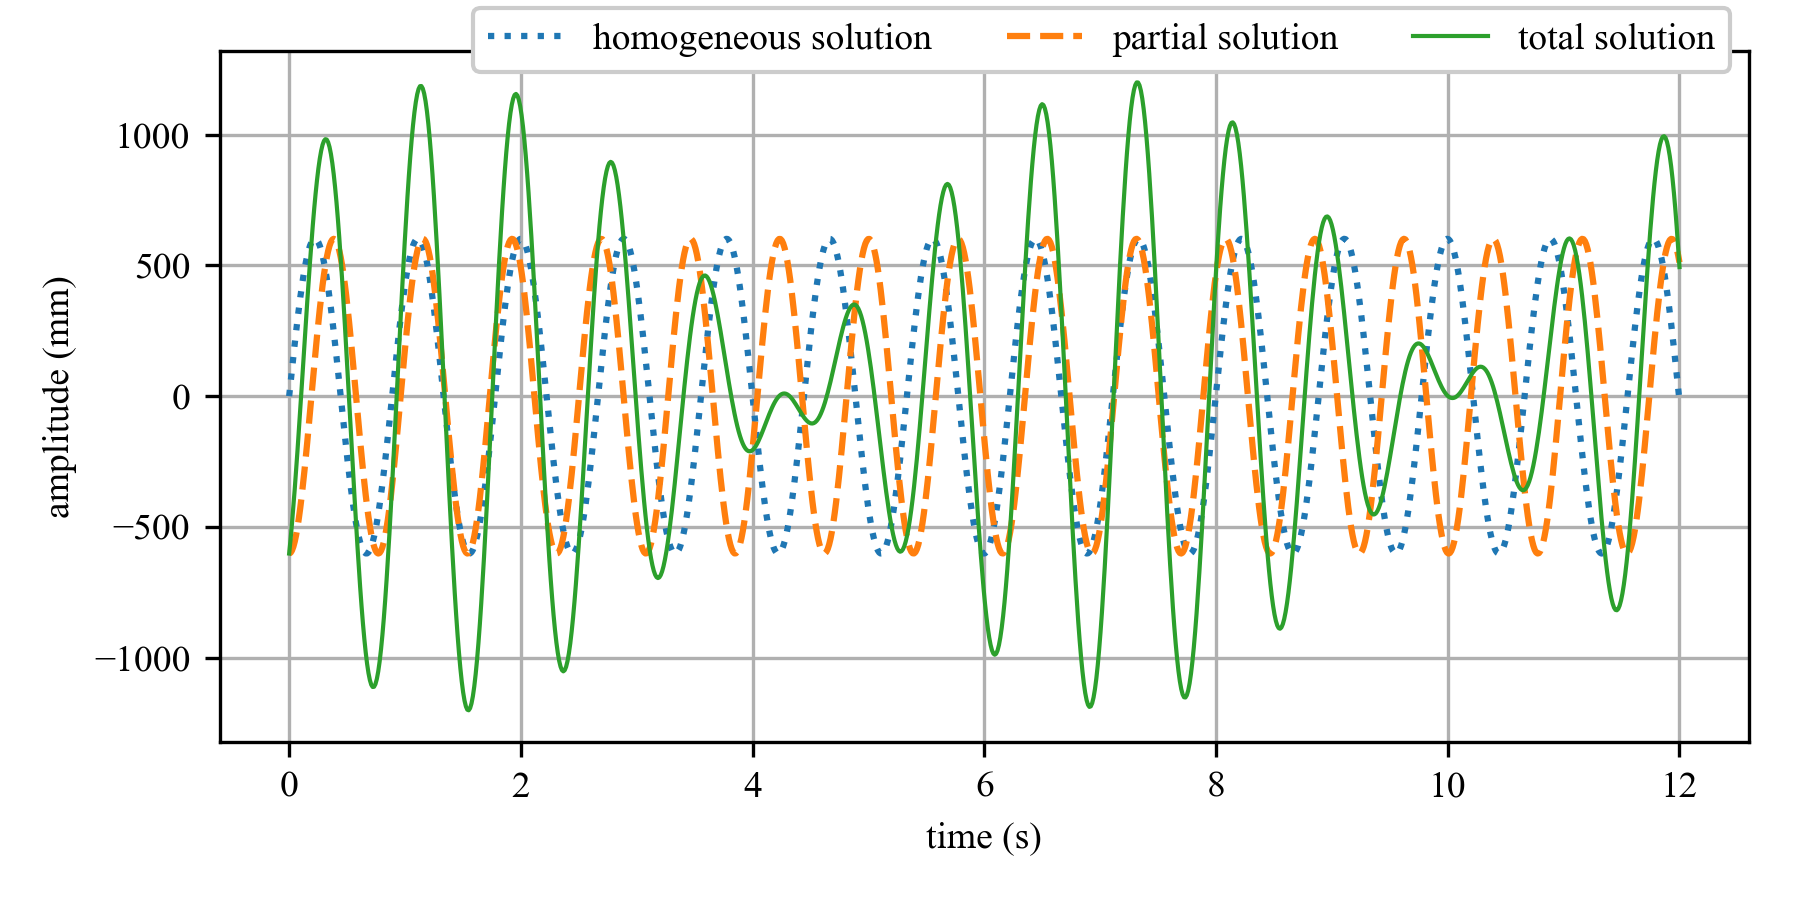
\includegraphics[]{../Figures/topic_6_example_1.png}
			\end{figure}			

\end{example}

\begin{example}
			Considering the following system, write the equation of motion and calculate the response assuming a) that the system is initially at rest, and b) that the system has an initial displacement of 0.005 m. Use $k$ = 2000 N/m, $m$ = 100 kg, $F(t)$ = 10sin(10t) N.
			\begin{figure}[H]
				\centering
				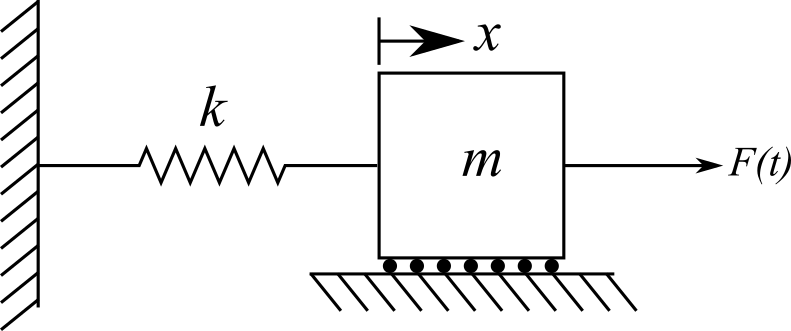
\includegraphics[width=0.5\textwidth]{../Figures/forced_spring_mass_system.png}
			\end{figure}
			The equation of motion is
			\begin{equation}
				m\ddot{x}+kx=10\text{sin}(10t)
			\end{equation}
			or in standard form:
			\begin{equation}
				\ddot{x}+\omega_n^2x=f_0\text{sin}(\omega t)
			\end{equation}							
			Note that the forcing function is in terms of sin, not cos as before, so we will have to resolve for the constants $A_1$ and $A_2$. Again, setting the particular solution to $x_p=X\text{sin}(\omega t)$ and solving for $X$ as before yields:
			\begin{equation}
				x(t) = A_1\text{sin}(\omega_n t) + A_2\text{cos}(\omega_n t) + \frac{f_0}{\omega_n^2-\omega^2}\text{sin}(\omega t)
			\end{equation}	
			Now we can solve for $A_1$ and $A_2$ by setting the initial conditions $x_0$ and $v_0$ to $t=0$. First, setting $t=0$ in the equation for $x(t)$ yields:
			\begin{equation}
				A_2 = x_0
			\end{equation}	
			Then, a function for the velocity of the system is obtained: 
			\begin{equation}
				\dot{x}(t) = v_0 = A_1\omega_n\text{cos}(\omega_n t) - A_2\omega_n\text{sin}(\omega_n t) + \omega\frac{f_0}{\omega_n^2-\omega^2}\text{cos}(\omega t)
			\end{equation}				
			This allows us to obtains:
			\begin{equation}
				A_1 = \frac{v_0}{\omega_n}-\frac{\omega}{\omega_n}\cdot \frac{f_0}{\omega_n^2-\omega^2}
			\end{equation}	
			at $t=0$. These lead to the full equation for the general solution:
			\begin{equation}
				x(t) = \Big(\frac{v_0}{\omega_n}-\frac{\omega}{\omega_n}\cdot \frac{f_0}{\omega_n^2-\omega^2}\Big)\text{sin}(\omega_n t) + x_0\text{cos}(\omega_n t) + \frac{f_0}{\omega_n^2-\omega^2}\text{sin}(\omega t)
			\end{equation}								
			Also, knowing:
			\begin{equation}
				\omega_n = \sqrt{\frac{k}{m}} = \sqrt{20} \text{ rad/sec} =  4.472 \text{ rad/sec}
			\end{equation}				
			and
			\begin{equation}
				f_o = \frac{F_0}{m} = \frac{F_0}{m} = 0.1 \text{ N/kg}
			\end{equation}	
			a) using the initial conditions $x_0$ = 0 m and $v_0$ = 0 m/s and the general expression obtained above:
			\begin{equation}
				x(t) = \Big(0-\frac{10}{\sqrt{20}}\cdot \frac{0.1}{20-10^2}\Big)\text{sin}(\sqrt{20} t) + 0 + \frac{0.1}{20-10^2}\text{sin}(10 t)
			\end{equation}			
			b) using the initial conditions $x_0$ = 0.005 m and $v_0$ = 0 m/s and the general expression obtained above:
			\begin{equation}
				x(t) = \Big(0-\frac{10}{\sqrt{20}}\cdot \frac{0.1}{20-10^2}\Big)\text{sin}(\sqrt{20} t) + 0.05\text{cos}(\sqrt{20} t) + \frac{0.1}{20-10^2}\text{sin}(10 t)
			\end{equation}			
			\begin{figure}[H]
				\centering
				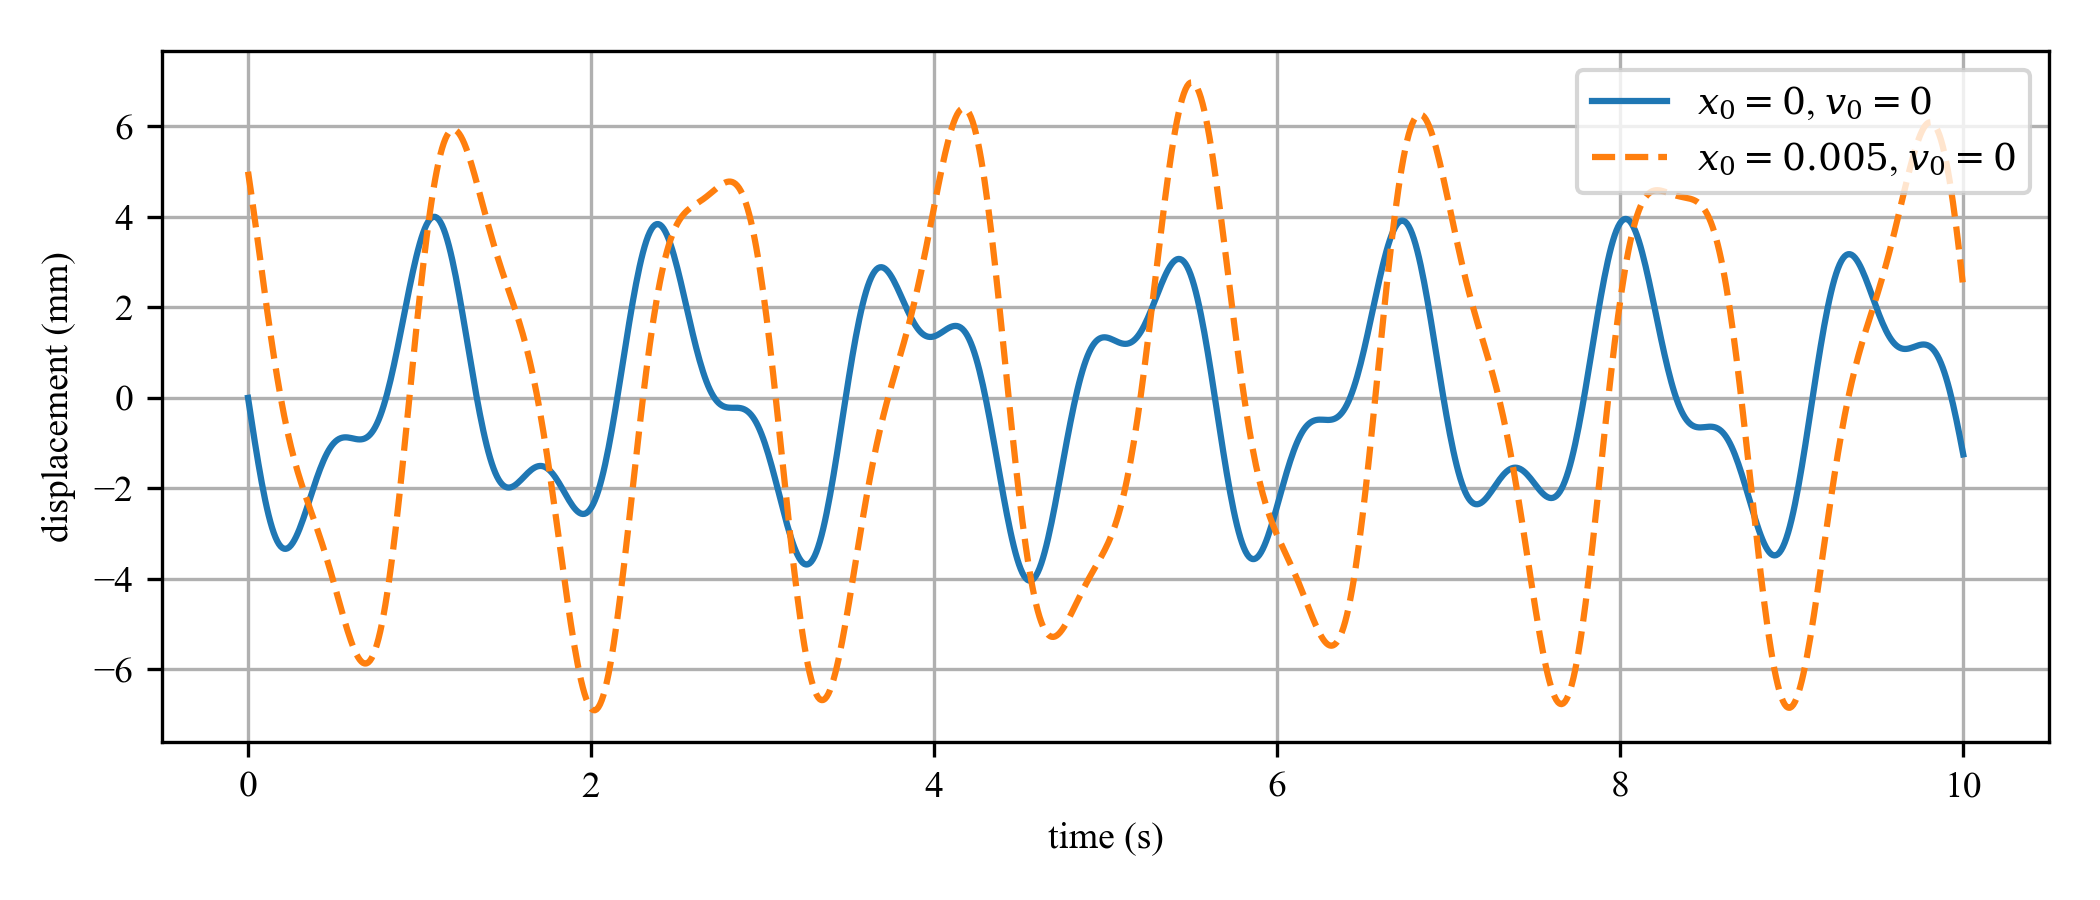
\includegraphics[width=1.0\textwidth]{../Figures/topic_6_example_2.png}
			\end{figure}
\end{example}


	
		\subsection{Harmonic excitations of underdamped systems}

			Consider the system
			\begin{figure}[H]
				\centering
				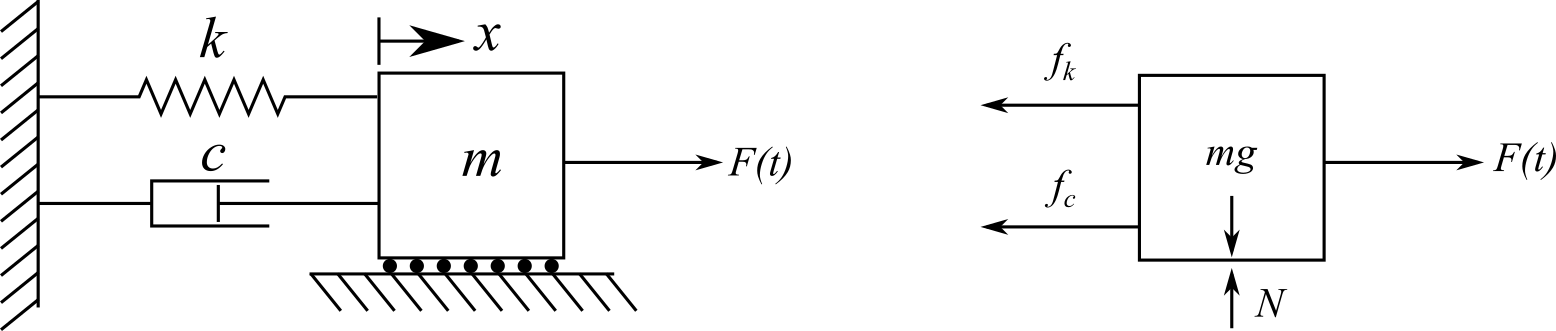
\includegraphics[width=0.7\textwidth]{../Figures/system_and_FBD_1DOF_damped_forced_horiziontal.png}
			\end{figure}	
			Again, for simplicity let us consider a harmonic excitation for $F(t)$ such that:
			\begin{equation}
				F(t) = F_0\text{cos}(\omega t)
			\end{equation}							
			Summing the forces in the above figure in the $x$ direction yields:
			\begin{equation}
				m \ddot{x}(t)+c\dot{x}(t)+kx(t) = F_0\text{cos}(\omega t)
			\end{equation}			
			For convinces we can convert this to the standard form:					
			\begin{equation}
				\ddot{x}(t)+2 \zeta \omega_n \dot{x}(t) +\omega_n^2x(t) = f_0\text{cos}(\omega t)
			\end{equation}					
			again, where:
			\begin{equation}
				f_0 = \frac{F_0}{m}
			\end{equation}	
			Recall that one way to solve such an equation is to obtain the sum of the homogeneous and particular solutions. 
			\begin{equation}
				x(t) = x_h(t) + x_p(t)
			\end{equation}	
			However, now that we have damping force to consider, out partial solution will have to consider this damping. Therefore:
			\begin{equation}
				x_p(t) = X \text{cos}(\omega t - \phi_p)
			\end{equation}
			where $\phi_p$ represents the phase shift. Note: $\phi_p$ is represented in other texts as $\theta$, $\theta_p$, or even just $\phi$ but we will use $\phi_p$ throughout the remainder of this course. Again, the phase shift is expected because of the effect of the damping force. Now, our total equation is:
			\begin{equation}
				x(t) = Ae^{-\zeta \omega_n t}\text{sin}(\omega_d t + \phi) +  X \text{cos}(\omega t - \phi_p)
			\end{equation}			
			We can use the method of undetermined coefficients to obtain $X$ and $\phi_p$ for the partial solution. First, considering that we write the partial solution in equivalent form:
			\begin{equation}
				x_p(t) = X \text{cos}(\omega t - \phi_p) = A_s \text{cos}(\omega t) + B_s  \text{sin}(\omega t)
			\end{equation}			 
			Taking the derivative of the assumed forms of the partial solution yields:
			\begin{equation}
				x_p(t) = A_s \text{cos}(\omega t) + B_s  \text{sin}(\omega t)
			\end{equation}	
			\begin{equation}
				\dot{x}_p(t) = -\omega A_s \text{sin}(\omega t) + \omega B_s  \text{cos}(\omega t)
			\end{equation}				 
			\begin{equation}
				\ddot{x}_p(t) = -\omega^2 A_s \text{cos}(\omega t) - \omega^2 B_s  \text{sin}(\omega t)
			\end{equation}				
			Recall that the homogeneous and partial solutions are each solution on their own, therefor the EOM can be used to describe just the partial solution. Substituting $x_p$. $\dot{x}_p$, and $\ddot{x}_p$ for $x$. $\dot{x}$, and $\ddot{x}$ in the EOM in standard form $\ddot{x}(t)+2 \zeta \omega_n \dot{x}(t) +\omega_n^2x(t) = f_0\text{cos}(\omega t)$ yields:
			\begin{equation}
			 	\big(	-\omega^2 A_s \text{cos}(\omega t) - \omega^2 B_s  \text{sin}(\omega t) \big)(t)+2 \zeta \omega_n  \big( -\omega A_s \text{sin}(\omega t) + \omega B_s  \text{cos}(\omega t)  \big) (t) +
			\end{equation}
			\begin{equation*}
				\omega_n^2 \big( A_s \text{cos}(\omega t) + B_s  \text{sin}(\omega t) \big)(t) = f_0\text{cos}(\omega t)
			\end{equation*}				
			and rearranging in terms of sin($\omega t$) and cos($\omega t$) yields: 
			\begin{equation}
				(-\omega^2 A_s + 2 \zeta \omega_n \omega B_s + \omega_n^2 A_s -f_0) \text{cos}(\omega t) + 
			\end{equation}
			\begin{equation*}
				(-\omega^2 B_s - 2 \zeta \omega_n \omega A_s + \omega_n^2 B_s)\text{sin}(\omega t) =0
			\end{equation*}	
			considering the two special moments in time $t=(\pi/2)\omega$ and $t=0$ where cos($\omega t$) and sin($\omega t$) equal zero, respectively. Considering $t=(\pi/2)\omega$ results in cos($\omega t$)=0, sin($\omega t$)=1 and the equation simplifies to:
			\begin{equation}
				(-2\zeta \omega_n \omega)A_s + (\omega_n^2 - \omega^2)B_s = 0
			\end{equation}	
			Additionally, at $t=0$, sin($\omega t$)=0 and cos($\omega t$)=1. Therefore, the equation yields		
			\begin{equation}
				(\omega_n^2 - \omega^2)A_s + (2\zeta \omega_n \omega)B_s = f_0
			\end{equation}				
			We can solve two equations for two unknowns. Writing the two linear equations as the singular matrix equation yields:
			\begin{gather}
			   \begin{bmatrix}
			   \omega_n^2 - \omega^2 & 2\zeta \omega_n \omega \\
			   - 2\zeta \omega_n \omega &  \omega_n^2 - \omega^2
			   \end{bmatrix}
  			   \begin{bmatrix}
  			   A_s \\
  			   B_s
  			   \end{bmatrix}
			 = \begin{bmatrix} f_0 \\ 0
			 \end{bmatrix}
			\end{gather}
			This can be solved by computeing the complex inversing, to give us:
			\begin{equation}
				A_s = \frac{(\omega_n^2 - \omega^2)f_0}{(\omega_n^2 - \omega^2)^2 +  (2\zeta \omega_n \omega)^2}
			\end{equation}	
			\begin{equation}
				B_s = \frac{2\zeta \omega_n \omega f_0}{(\omega_n^2 - \omega^2)^2 +  (2\zeta \omega_n \omega)^2}
			\end{equation}	
			From out trigonometric relationships, 
			\begin{equation}
				X = \sqrt{A_s^2 + B_s^2}
			\end{equation}	
			\begin{equation}
				\phi_p = \text{tan}^-1\bigg(\frac{B_s}{A_s}\bigg)
			\end{equation}	
			We can now derive values for our partial solution $x_p$:
			\begin{equation}
				X = \frac{f_0}{\sqrt{(\omega_n^2 - \omega^2)^2 +  (2\zeta \omega_n \omega)^2}} 
			\end{equation}	
			\begin{equation}
				\phi_p = \text{tan}^-1\bigg(\frac{2\zeta \omega_n \omega}{\omega_n^2 - \omega^2}\bigg)
			\end{equation}				
			Now we can build a solution for the partial equation ($x_p$), therefore, the total solution becomes:
			\begin{equation}
				x(t) = x_h(t) + x_p(t)
			\end{equation}
			\begin{equation}
				x(t) = Ae^{-\zeta \omega_n t}\text{sin}(\omega_d t + \phi) +  X \text{cos}(\omega t - \phi_p)
			\end{equation}				
			Note for larger values of $t$, the homogeneous solution approaches zero resulting in the partial solution becoming the total solution. Therefore, the partial solution is sometimes called the \textbf{steady state response} and the homogeneous solution is called the \textbf{transient response}. Solving for the constants $A$ and $\phi$ using boundary conditions ($x_0=0$ and $v_0=0$) results a total solution expressed as:
			\begin{equation}
				A = \frac{x_0 -X \text{cos}(\phi_p)}{\text{sin}(\phi)}
			\end{equation}			 
			\begin{equation}
				\phi =  \text{tan}^-1\bigg(\frac{\omega_d ( x_0 -X \text{cos}(\phi_p))}{v_0 + (x_0 - X \text{cos}(\phi_p)) \zeta \omega_n - \omega X \text{sin}(\phi_p) }\bigg)
			\end{equation}			
			Finally, assembling all the terms:
			\begin{equation}
				x(t) = Ae^{-\zeta \omega_n t}\text{sin}(\omega_d t + \phi) +  X \text{cos}(\omega t - \phi_p)
			\end{equation}
			\begin{equation}
				A = \frac{x_0 -X \text{cos}(\phi_p)}{\text{sin}(\phi)}
			\end{equation}			 
			\begin{equation}
				\phi =  \text{tan}^-1\bigg(\frac{\omega_d ( x_0 -X \text{cos}(\phi_p))}{v_0 + (x_0 - X \text{cos}(\phi_p)) \zeta \omega_n - \omega X \text{sin}(\phi_p) }\bigg)
			\end{equation}	
			\begin{equation}
				X = \frac{f_0}{\sqrt{(\omega_n^2 - \omega^2)^2 +  (2\zeta \omega_n \omega)^2}} 
			\end{equation}	
			\begin{equation}
				\phi_p = \text{tan}^-1\bigg(\frac{2\zeta \omega_n \omega}{\omega_n^2 - \omega^2}\bigg)
			\end{equation}							
			Let's consider how these equation play out in a real system. Again, consider the system
			\begin{figure}[H]
				\centering
				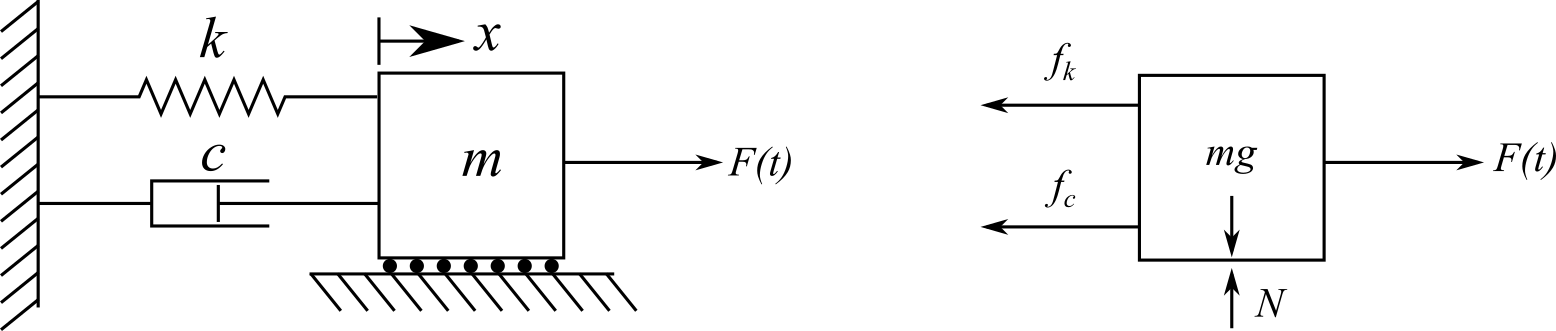
\includegraphics[width=0.7\textwidth]{../Figures/system_and_FBD_1DOF_damped_forced_horiziontal.png}
			\end{figure}			
			If we plot the total, transient, and steady state responses for $k=100$ N/m, $m=10$ kg,  $c=10$ kg/s, $F_0=1$ N, $\omega=3.162$ rad/sec, and no initial conditions we get:
			\begin{figure}[H]
				\centering
				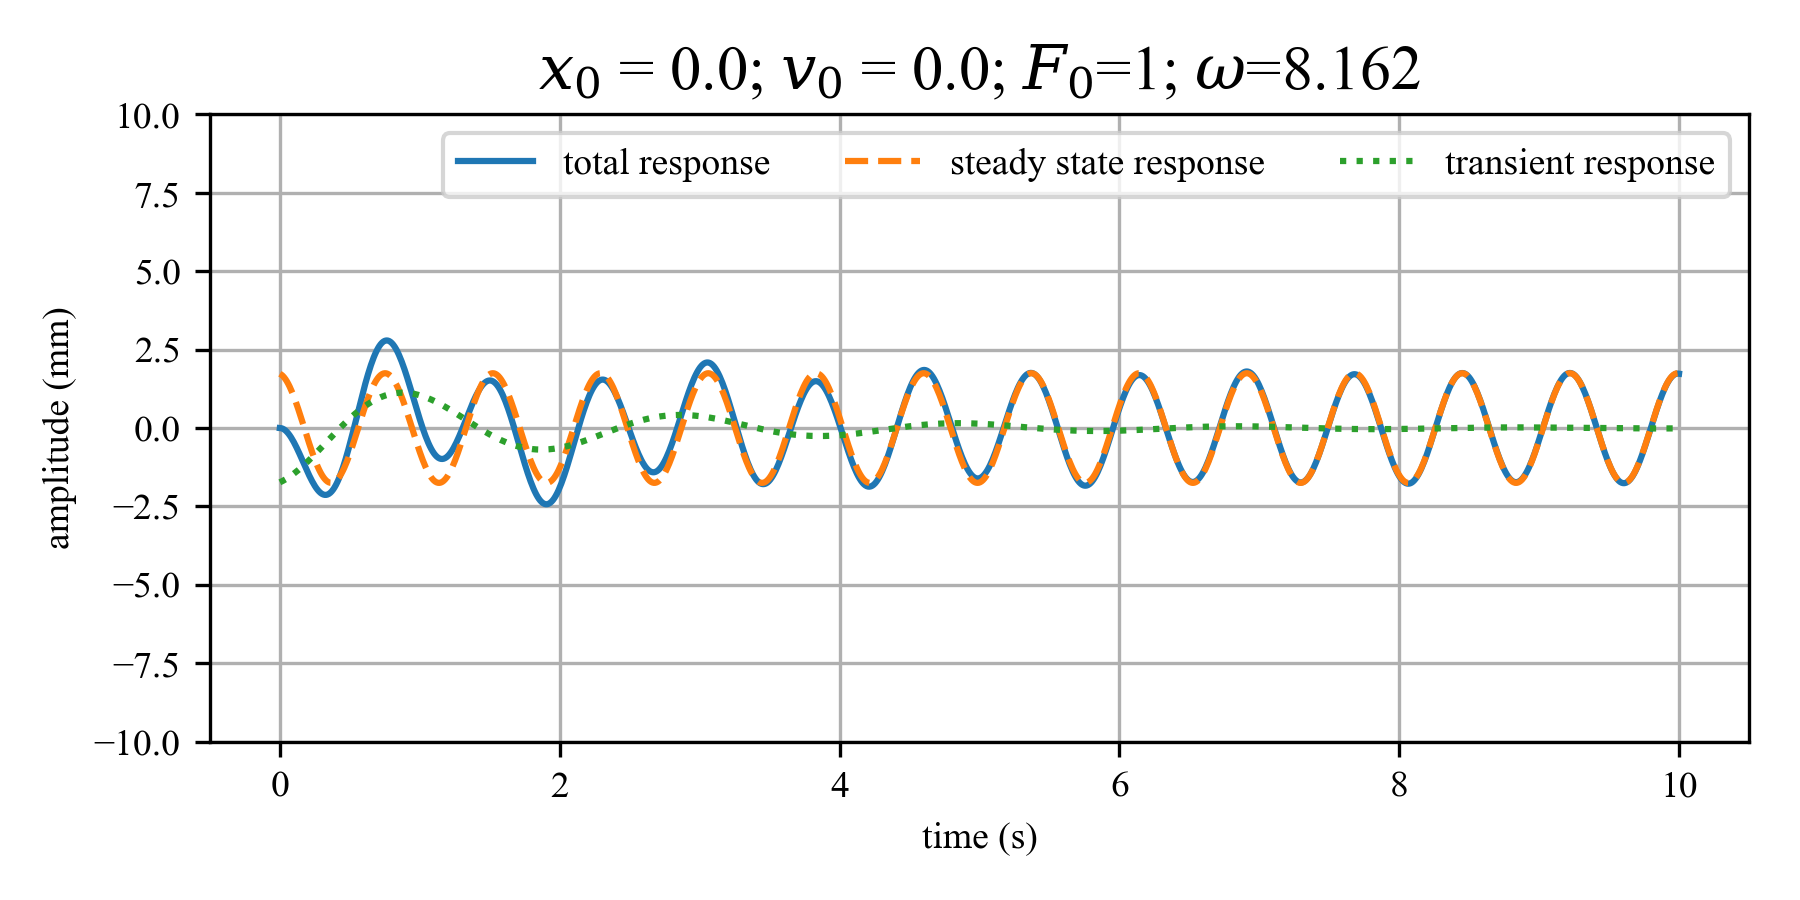
\includegraphics[width=0.7\textwidth]{../Figures/example_1_1.png}
			\end{figure}			
			If we increase the forcing function $F_0$ to 3 N we get:
			\begin{figure}[H]
				\centering
				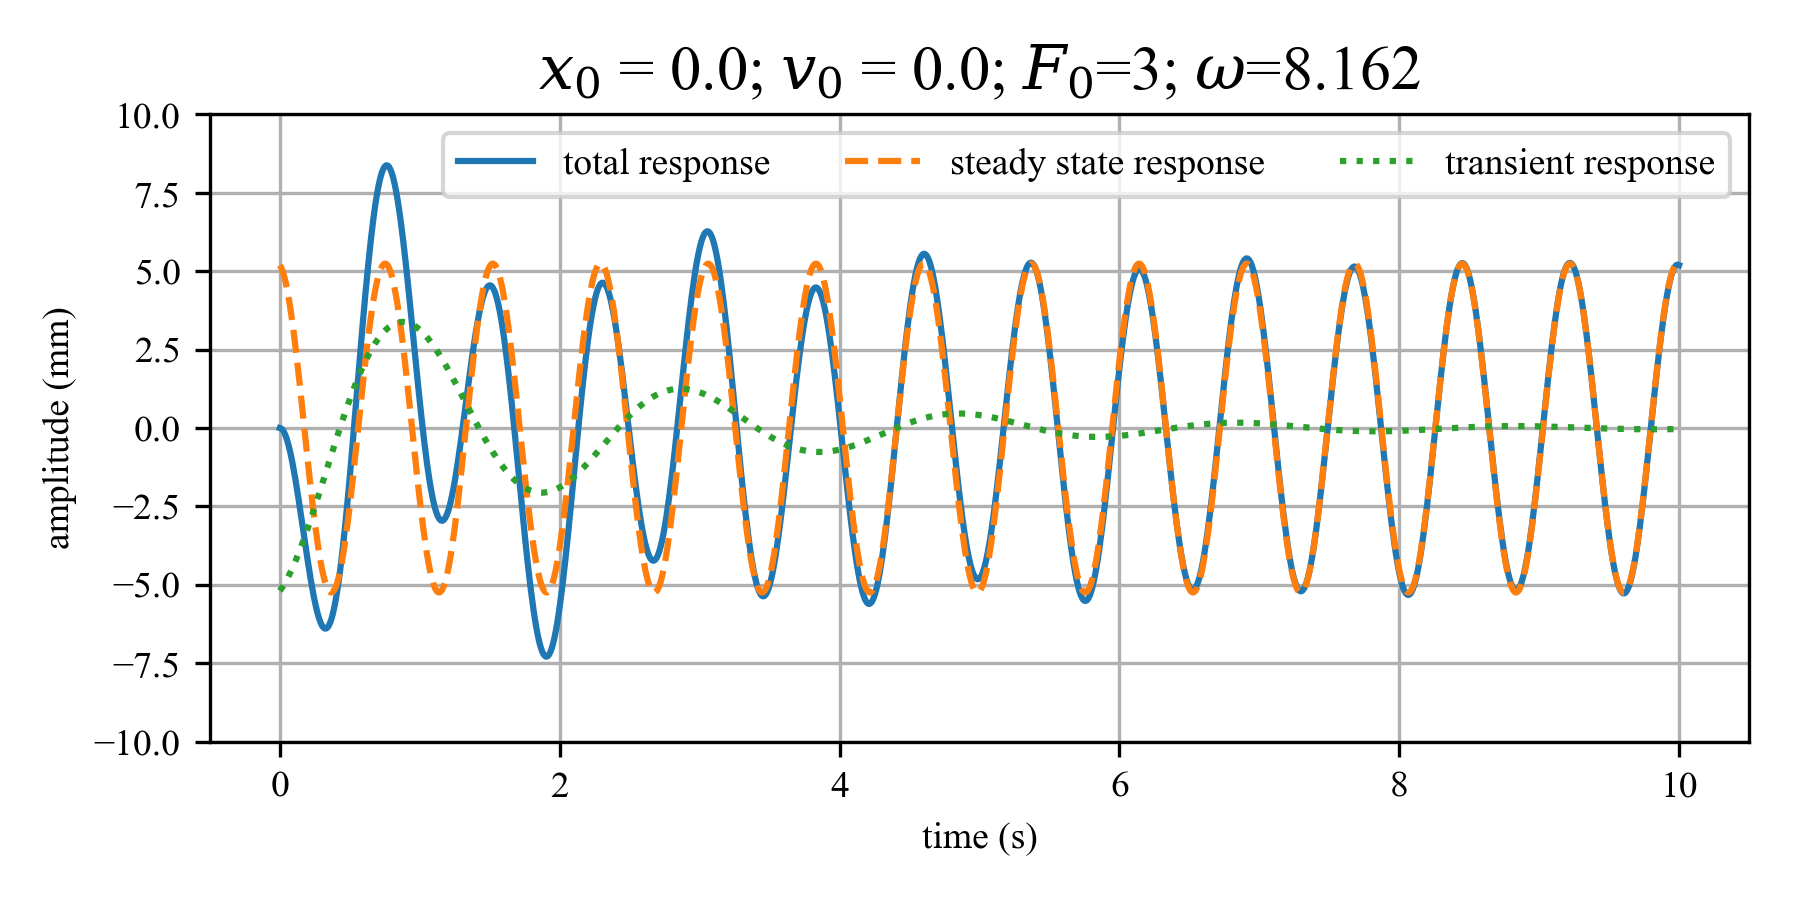
\includegraphics[width=0.7\textwidth]{../Figures/example_1_2.png}
			\end{figure}			
			now, using $F_0=1$ N, but setting $\omega=5$ rad/sec we get:
			\begin{figure}[H]
				\centering
				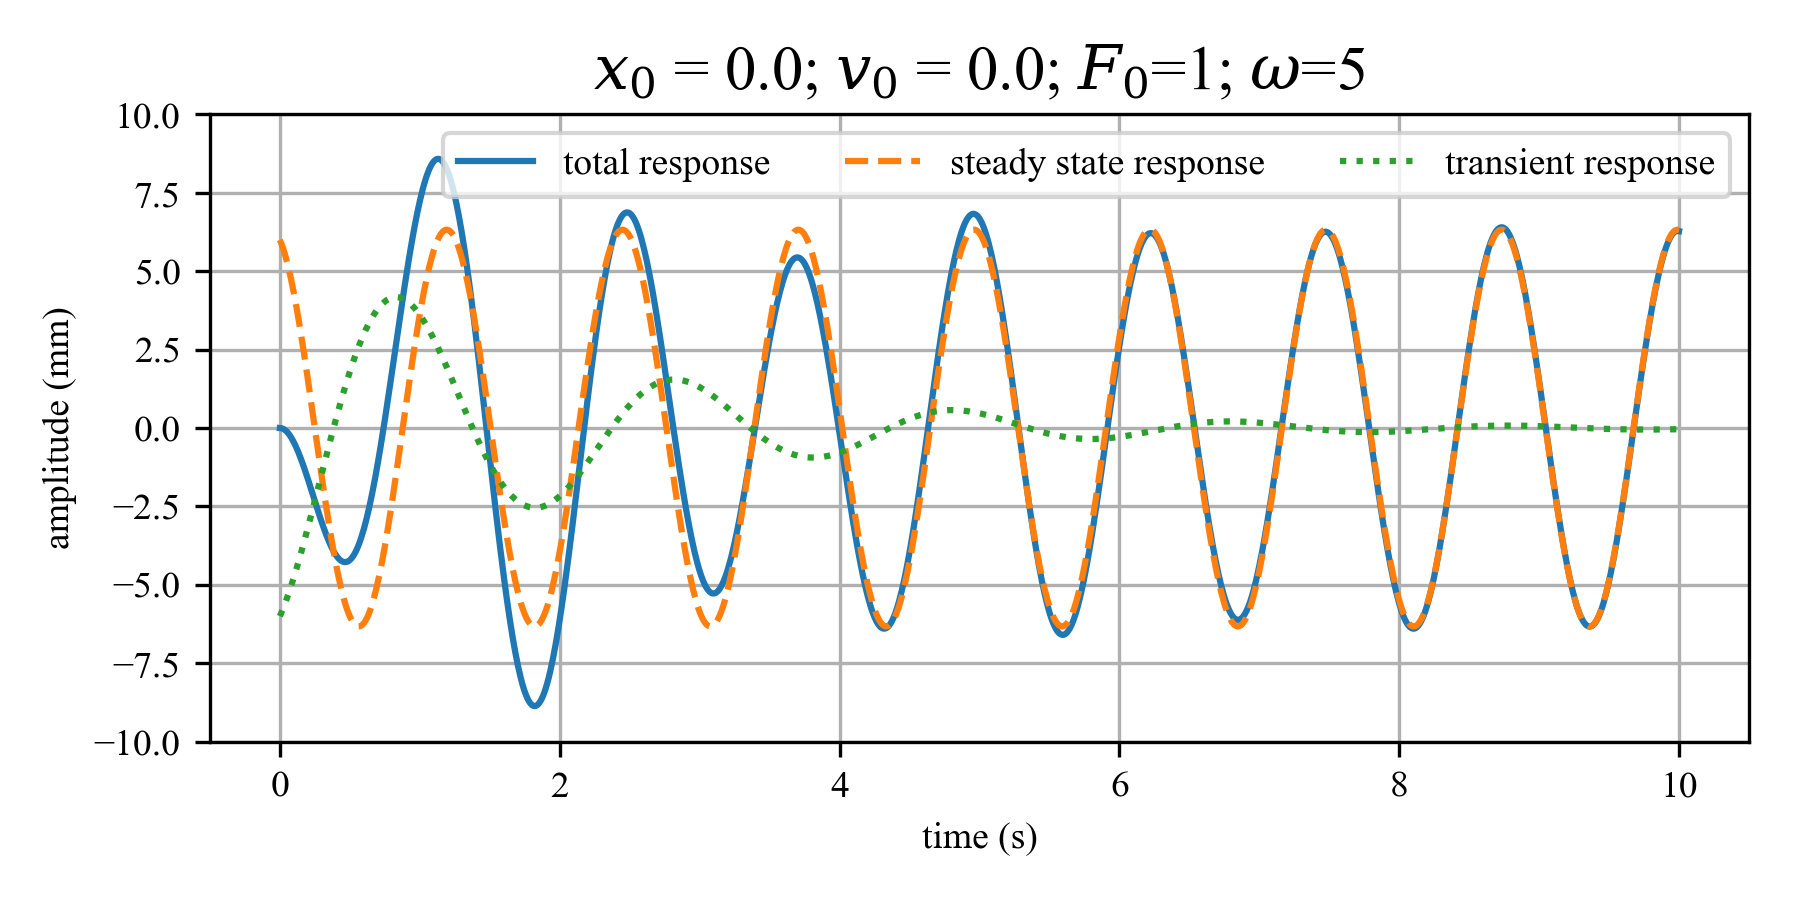
\includegraphics[width=0.7\textwidth]{../Figures/example_1_3.png}
			\end{figure}				
			This is because $\omega$ is closer to the natural frequency $\omega_n$. Setting $\omega=\omega_n$ we get
			\begin{figure}[H]
				\centering
				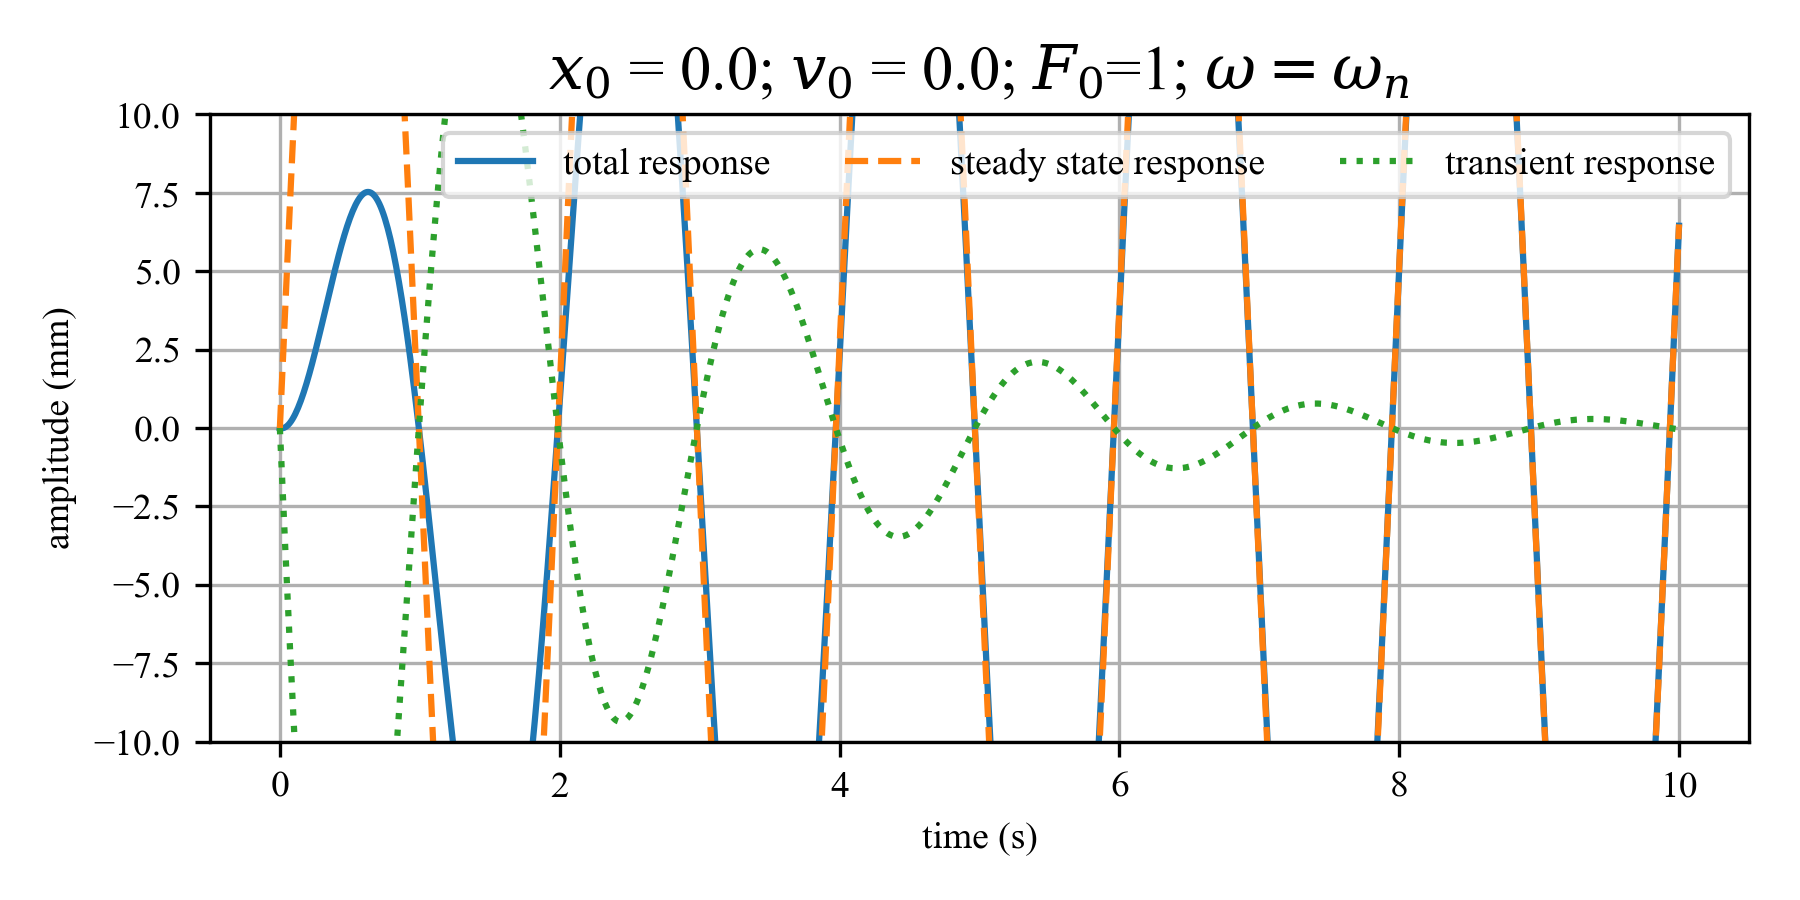
\includegraphics[width=0.7\textwidth]{../Figures/example_1_4.png}
			\end{figure}			
			As expected, setting $\omega=\omega_n$ causes the system to enter into resonance. However, this is different than resonance for a undamped system in that the amplitude of the displacement is not unbounded (recall that the damper will absorb energy). So if we scale the plot correctly we get: 
			\begin{figure}[H]
				\centering
				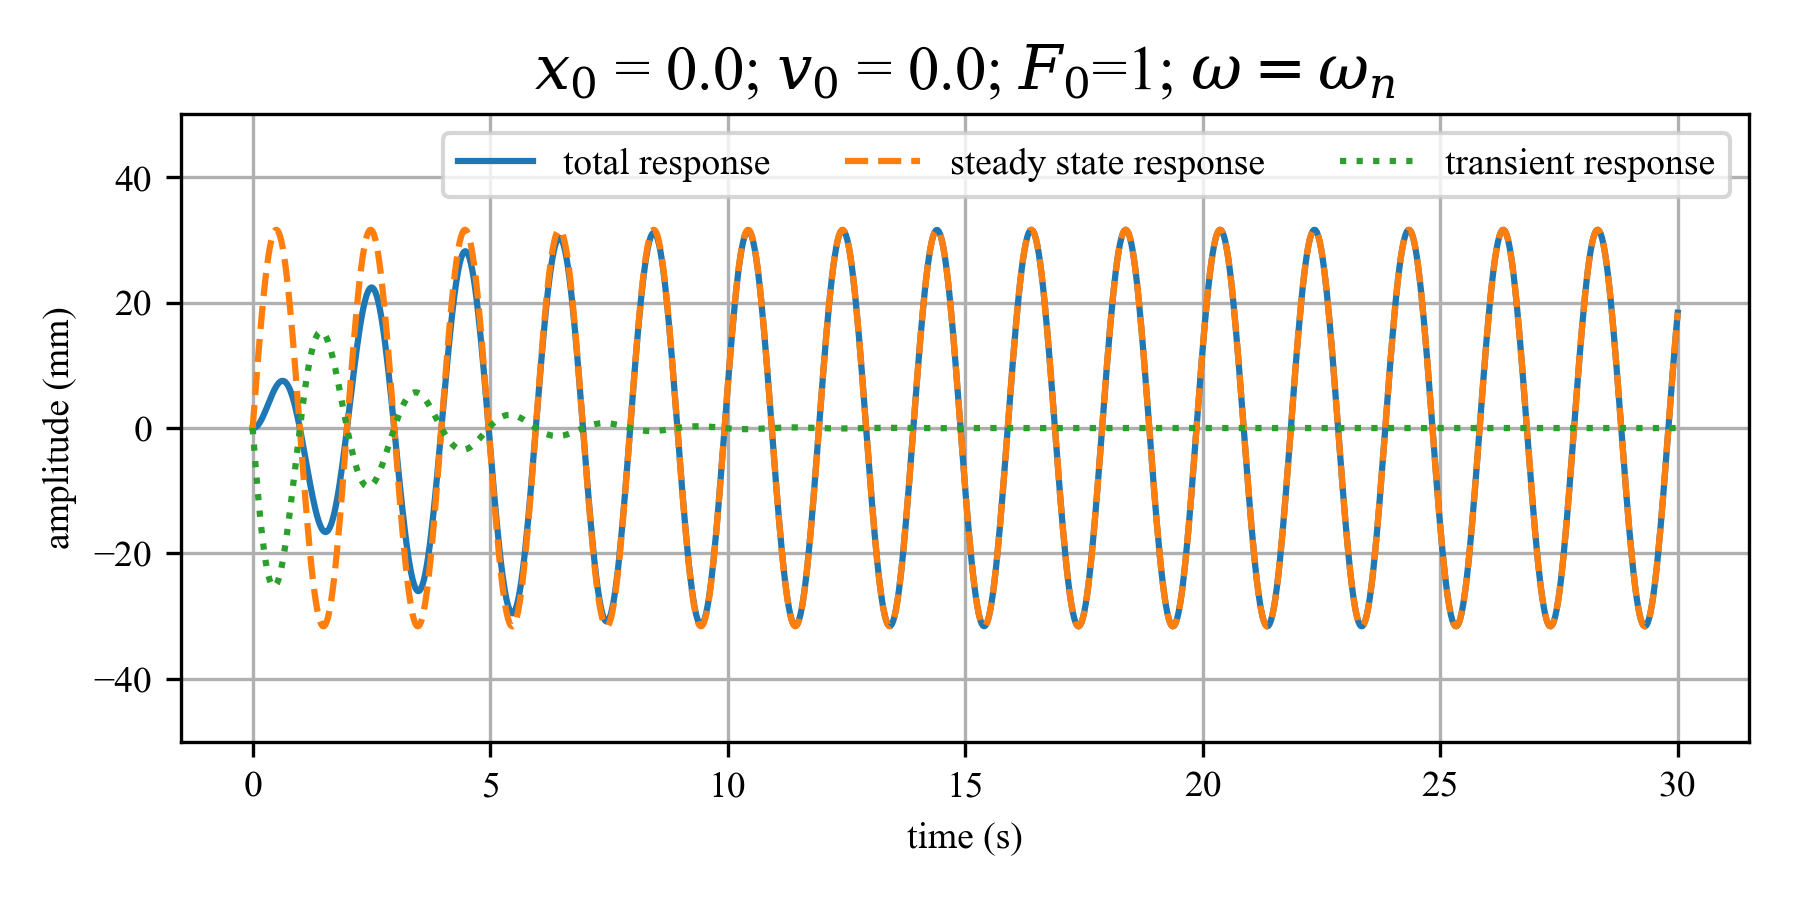
\includegraphics[width=0.7\textwidth]{../Figures/example_1_5.png}
			\end{figure}
			
			From the figure we can see that for larger values of $t$ the transient response dies out while only the steady state response controls the displacement of the total response. This is always true if the system has any significant damping. Therefore, it is often prudent to ignore the transient part and focus only on the steady-state response. Considering the equation for the partial solution: 
			\begin{equation}
				x_p(t) = X \text{cos}(\omega t - \phi_p)
			\end{equation}			 
			and knowing the values for $X$ and $\phi_p$: 
			\begin{equation}
				X = \frac{f_0}{\sqrt{(\omega_n^2 - \omega^2)^2 +  (2\zeta \omega_n \omega)^2}} 
			\end{equation}	
			\begin{equation}
				\phi_p = \text{tan}^-1\bigg(\frac{2\zeta \omega_n \omega}{\omega_n^2 - \omega^2}\bigg)
			\end{equation}	
			We want to find a way to plot the responses of the system only in terms of terms of the system's natural and driving frequencies, and its damping. First, we define a frequency ratio as the dimensionless quantity 
			\begin{equation}
				r = \frac{\omega}{\omega_n}
			\end{equation}
			\textbf{Another common way to express $r$ is $\beta$}. Next, Recall that:
			\begin{equation}
				X = \frac{f_0}{\sqrt{(\omega_n^2 - \omega^2)^2 +  (2\zeta \omega_n \omega)^2}}  = \frac{\frac{F_0}{m}}{\sqrt{(\omega_n^2 - \omega^2)^2 +  (2\zeta \omega_n \omega)^2}} 
			\end{equation}				
			If we factor out $\omega_n^2$ from the denominator and substitute in $\omega_n^2 = k/m$ and $r = \omega/\omega_n$, we get:
			\begin{equation}
				X = \frac{\frac{F_0}{m}}{\omega_n^2 \sqrt{\big(1 - (\frac{\omega}{\omega_n})^2\big)^2 +  (2\zeta \frac{\omega}{\omega_n})^2}} =  \frac{\frac{F_0}{k}}{\sqrt{(1-r^2)^2+(2\zeta r)^2}}
			\end{equation}				
			this becomes:
			\begin{equation}
				\frac{Xk}{F_0} = \frac{X \omega_n^2}{f_0} = \frac{1}{\sqrt{(1-r^2)^2+(2\zeta r)^2}}
			\end{equation}				
			in a similar fashion, if we manipulate the equation for $\phi_p$ we can get $\phi_p$ in term of $r$:
			\begin{equation}
				\phi_p = \text{tan}^-1\bigg(\frac{2 \zeta r}{1-r^2}\bigg)
			\end{equation}	
			If we solve for a few key values of $r$ we can get the following data points. On the board, we can solve for a few different frequency responses for a few different damping coefficients. 
			\begin{table}[H]
				\centering
				\begin{tabular}{@{}lccccccccc@{}}
				\toprule
				 & & \multicolumn{5}{c}{frequency ration ($r$)} \\ 
				$r$ & 0 & 0.25& 0.5& 0.75& 1& 1.25& 1.5& 1.75& 2.0 \\ \midrule
				$\zeta=0.7$	&	1.00&  1.00	&   0.97&	0.88&	0.71&	0.54&	0.41&	0.31 & 0.24\\
				$\zeta=0.5$	&	1.00&	1.03&	1.11&	1.15&	1.00&	0.73&	0.51&	0.37 & 0.28\\ 
				$\zeta=0.25$	&	1.00&	1.03&	1.11&	1.15&	1.00&	0.73&	0.51&	0.37 & 0.28 \\ 
				$\zeta=0.1$	&	1.00&	1.07&	1.32&	2.16&	5.00&	1.62&	0.78&	0.48 & 0.33 \\ \bottomrule
				\end{tabular}
			\end{table}
			If we plot the values of the normalize amplitude vs $r$ we obtain:
			\begin{figure}[H]
				\centering
				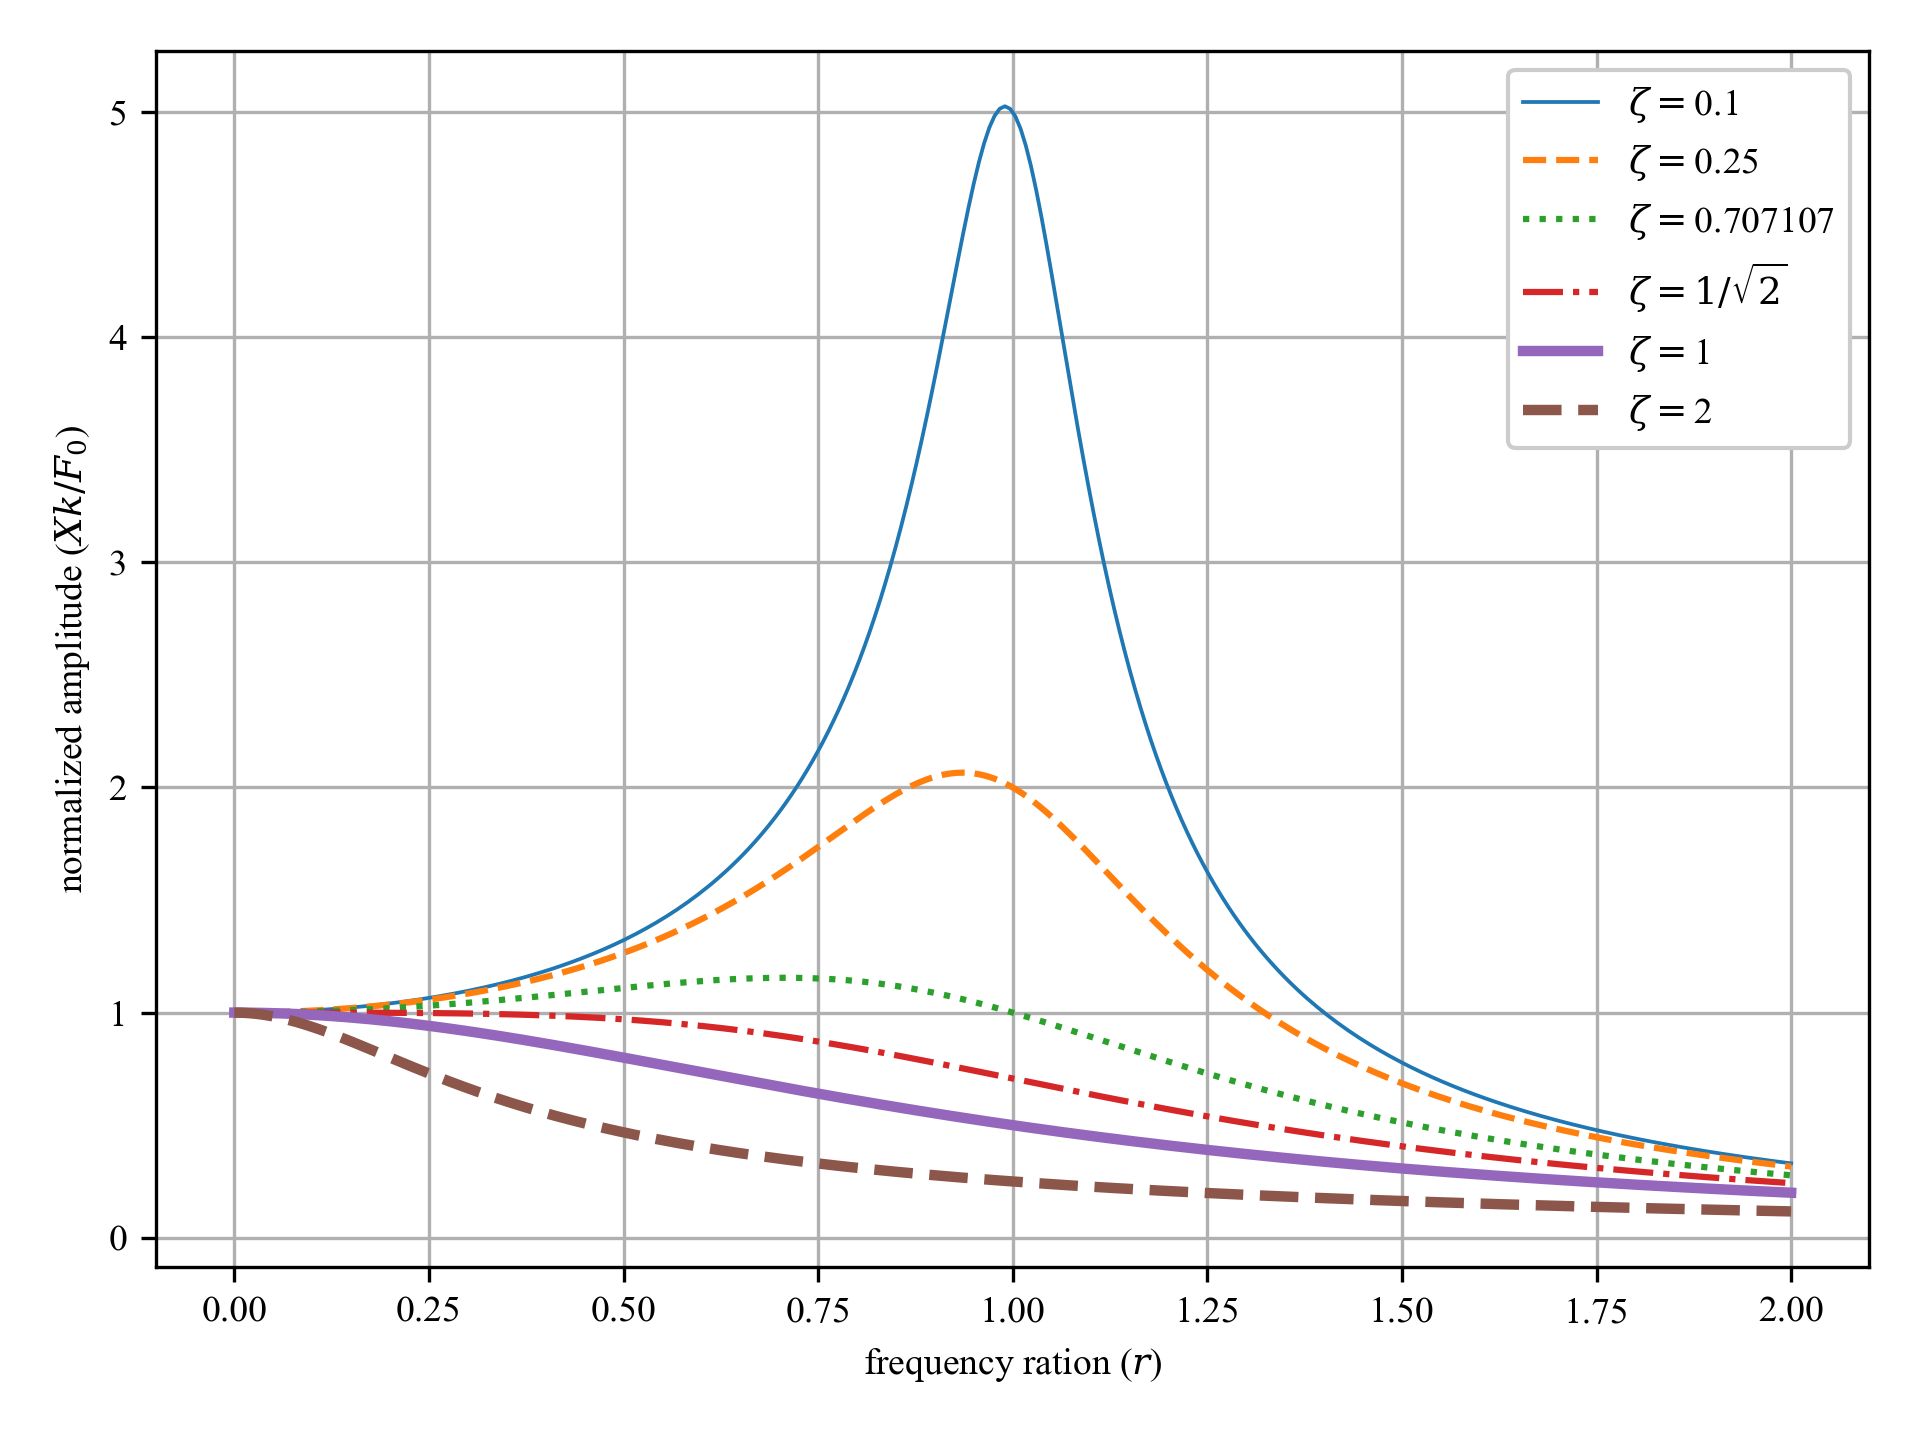
\includegraphics[width=0.8\textwidth]{../Figures/frequency_response_amplitude.png}
			\end{figure}			
			And again, if we plot the values of the phase vs $r$ ($\omega/\omega_n$) we obtain:
			\begin{figure}[H]
				\centering
				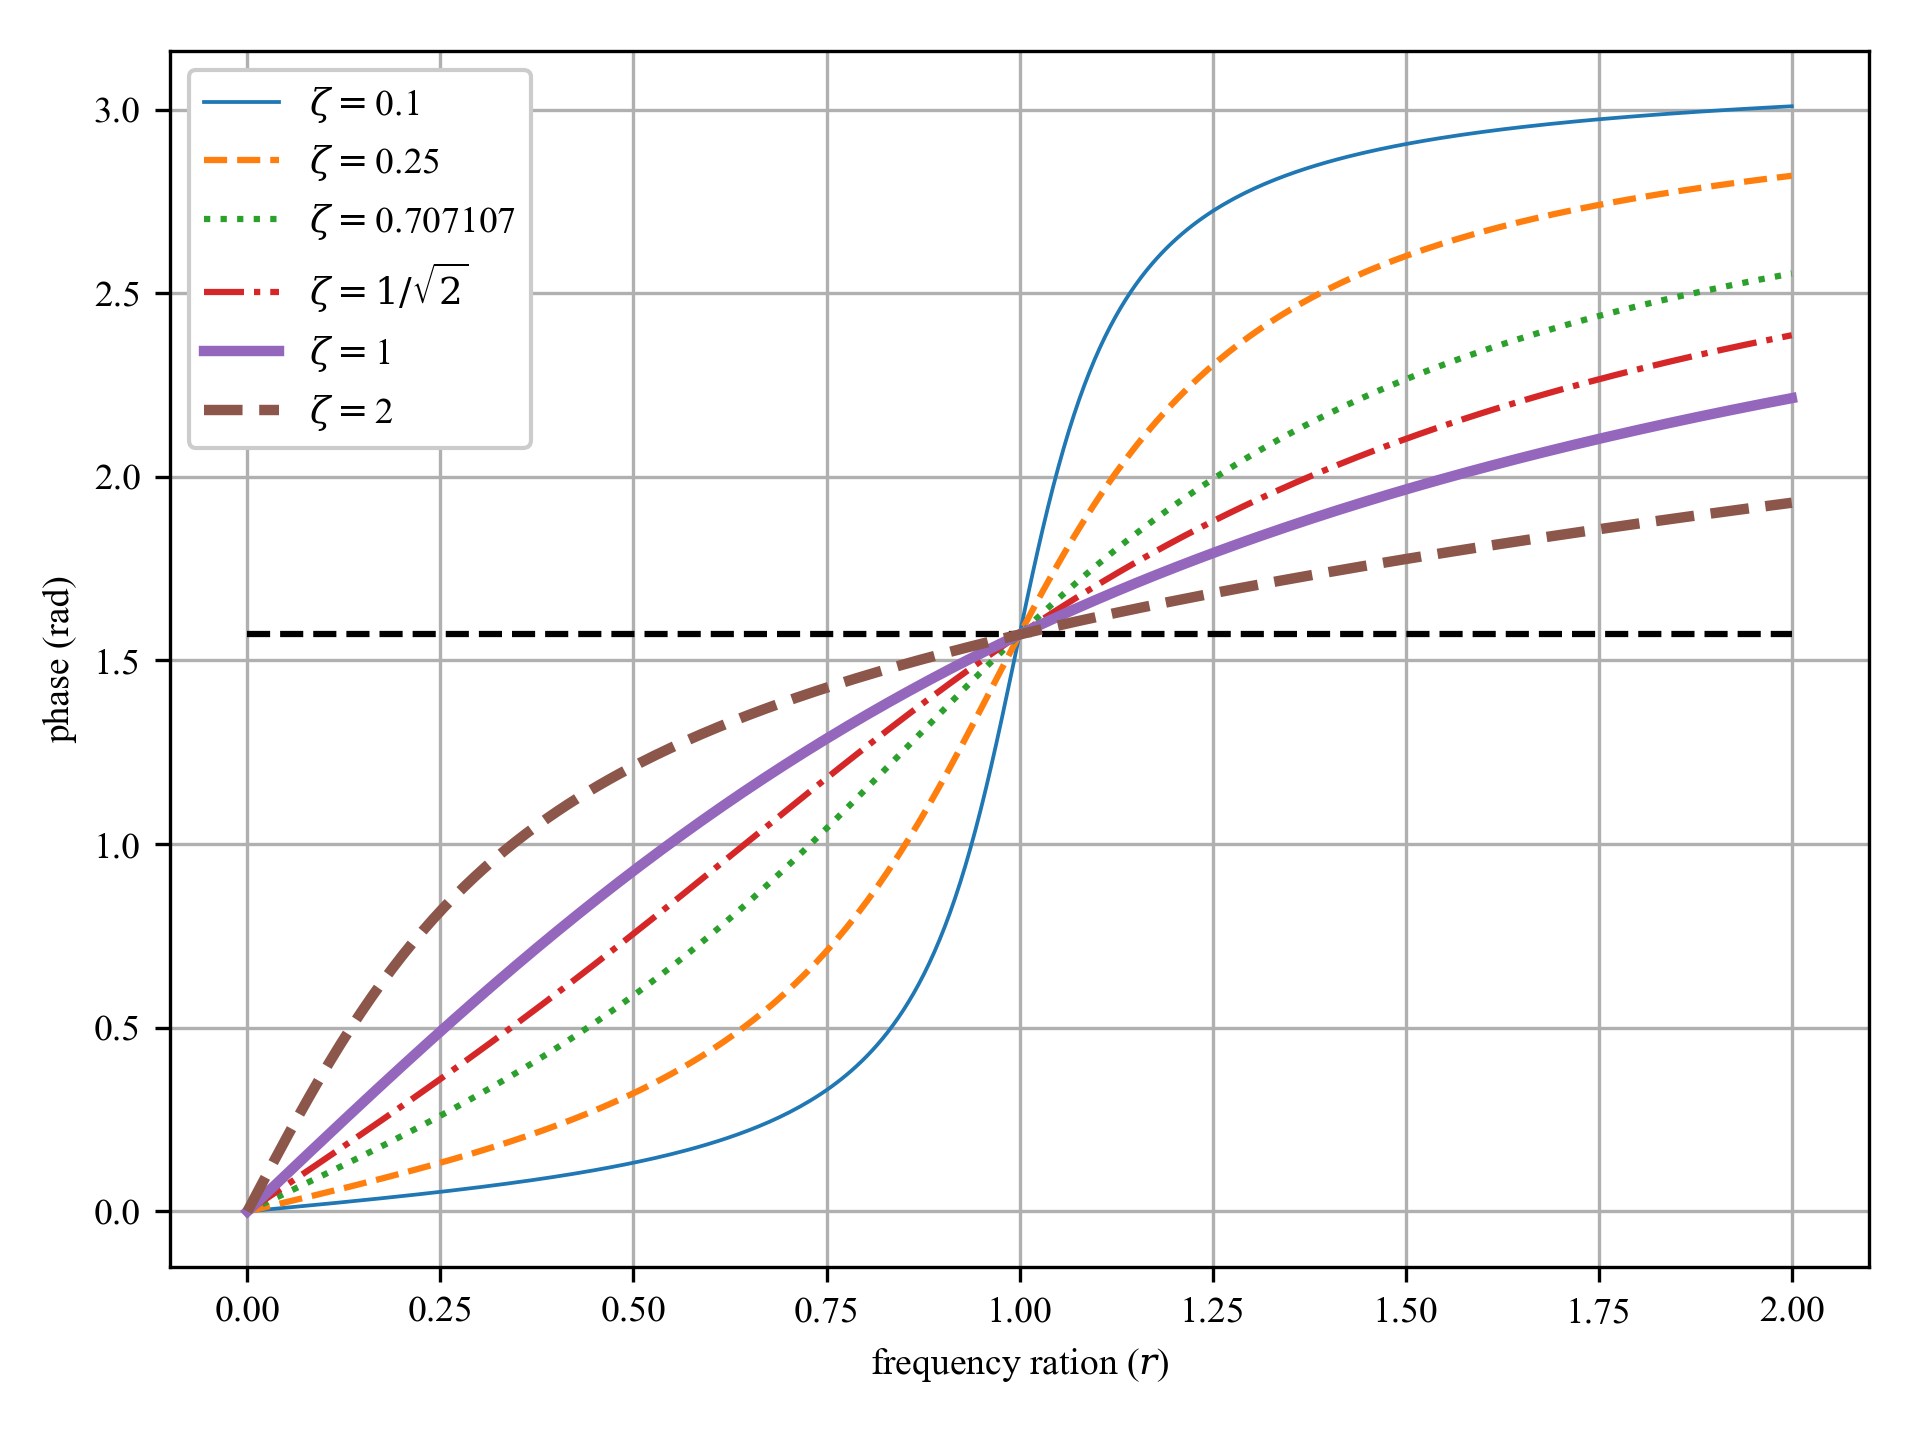
\includegraphics[width=0.8\textwidth]{../Figures/frequency_response_phase.png}
			\end{figure}				
			note that the dashed black line is there because the phase value after $\pi/2$ need to be adjusted to obtain a continuous plot. An astute observer would notice that the maximum amplitude is not at $\omega = \omega_n$. While resonance is defined as $\omega = \omega_n$, this does not define the point of maximum displacement of the steady state response. Let us solve for the frequency ratio with the maximum displacement. This will happen when
			\begin{equation}
				\frac{d}{dr}\Bigg(\frac{Xk}{F_0} \Bigg)= 0
			\end{equation}				
			We can show that:
			\begin{equation}
			\Bigg(\frac{1}{\sqrt{(1-r^2)^2+(2\zeta r)^2}}\Bigg)	\frac{d}{dr} =0
			\end{equation}	
			when 
			\begin{equation}
			r_{\text{peak}} = \sqrt{1-2 \zeta^2}= \frac{\omega_p}{\omega_n}, \hspace{1cm} \zeta<1/\sqrt{2} 
			\end{equation}				
			however, this is only true for under damped system in which $\zeta<1/\sqrt{2}$. If $\zeta>1/\sqrt{2}$ than the value in imaginary and the peak value is at $r=0$. In these cases, the maximum displacement is a function of only $\omega_n$. $\omega_p$ represents the driving frequency that correspond to the maximum amplitude ($\frac{Xk}{F_0}$) and is called the \textbf{peak frequency}, and can be calculated as:
			\begin{equation}
			\omega_p = \omega_n r_{\text{peak}} = \omega_n \sqrt{1-2 \zeta^2}, \hspace{1cm} \zeta<1/\sqrt{2} 
			\end{equation}				
			
			
			
\begin{example}

			Consider the simple spring mass system, 
			\begin{figure}[H]
				\centering
				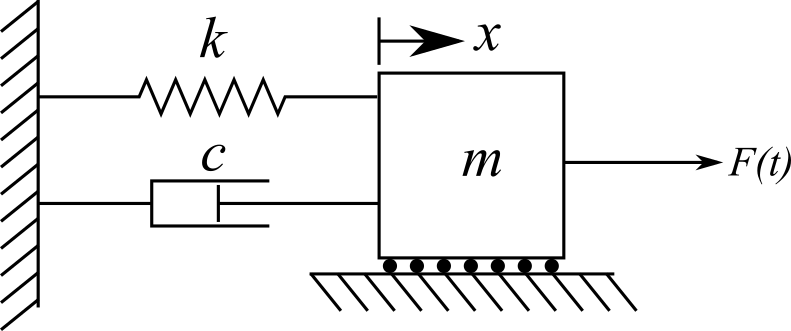
\includegraphics[width=0.4\textwidth]{../Figures/system_1DOF_horiziontal_damped_forced.png}
			\end{figure}				
			where $\omega_n = 132$ rad/sec and $\zeta$ = 0.0085. Calculate the displacements of the steady-state response for $\omega$=132 and 125 rad/sec. In both cases, use $f_0$ = 10 N/kg. 

			\textbf{Solution}
			
			From before, we know the solution for the displacement of the partial solution for $\omega$=132 rad/sec is:
			\begin{equation}
				X = \frac{f_0}{\sqrt{(\omega_n^2 - \omega^2)^2 +  (2\zeta \omega_n \omega)^2}} = \frac{10}{2(0.0085)(132)^2} = 0.034 \text{ m}
			\end{equation}							
			while for $\omega$=125 rad/sec X is:
			\begin{equation}
				X = \frac{f_0}{\sqrt{(\omega_n^2 - \omega^2)^2 +  (2\zeta \omega_n \omega)^2}} = \frac{10}{\sqrt{(1799)^2 +  (280.5)^2}}  = 0.005 \text{ m}
			\end{equation}				
			Therefore, a slight change in the driving frequency (about 5\%) results in a 85\% change in the amplitude of the steady-state response. 
\end{example}

\begin{example}

		

			The steady state response for an engineered system must not surpass 1 cm, if the system can be modeled as the spring and mass system below, what value of $c$ must be used?  
			\begin{figure}[H]
				\centering
				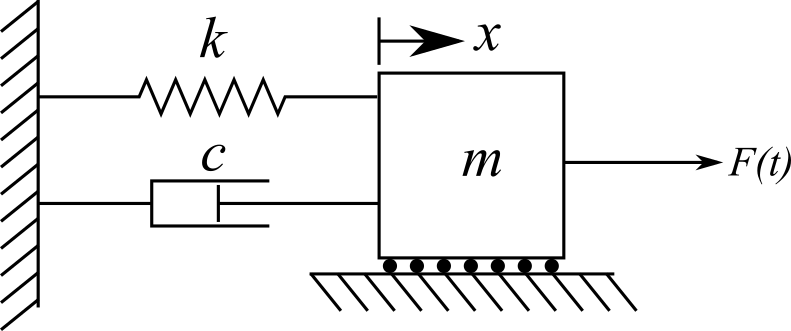
\includegraphics[width=0.4\textwidth]{../Figures/system_1DOF_horiziontal_damped_forced.png}
			\end{figure}	
			Use $k$ = 2000 N/m, $m$ = 100 kg, $F(t)$ = 20 cos($6.3t$) N. 			

			\textbf{Solution}
			The steady state solution is:
			\begin{equation}
				x_p(t) = X \text{cos}(\omega t - \phi_p)
			\end{equation}			 
			knowing the amplitude is controlled by $X$: 
			\begin{equation}
				X = \frac{f_0}{\sqrt{(\omega_n^2 - \omega^2)^2 +  (2\zeta \omega_n \omega)^2}} 
			\end{equation}	
			and recalling from the EOM in standard form that $2\zeta \omega_n = c/m$ we can obtain:
			\begin{equation}
				X = \frac{f_0}{\sqrt{(\omega_n^2 - \omega^2)^2 +  (\frac{c}{m} \omega)^2}} 
			\end{equation}		
			rearranging for $c$ gives:		
			\begin{equation}
				c = m\sqrt{\frac{f_0^2}{\omega^2 X^2}-\frac{\big(\omega_n^2-\omega^2\big)^2}{\omega^2}} = \sqrt{\frac{F_0^2}{\omega^2 X^2}-m^2\frac{\big(\omega_n^2-\omega^2\big)^2}{\omega^2}} 
			\end{equation}
			Therefore, if we set $X=0.01$ m we can solve the above equation to yield $c$ = 55.7 kg/s.
			
\end{example}	


	
		\subsection{Base excitation}

Often, loading is not applied directly to the mass, but rather the mass of the system is excited when the base of mount that it is attached to is excited. This is called base excitation, or sometimes support motion. Examples of base excitation, or where base excitation is considered, include:

\begin{itemize}
\item machines on rubber mounts
\item automobiles excited by the road
\item building under earthquake loading
\item hospital equipment
\end{itemize}

Consider the following system base excited system
\begin{figure}[H]
	\centering
	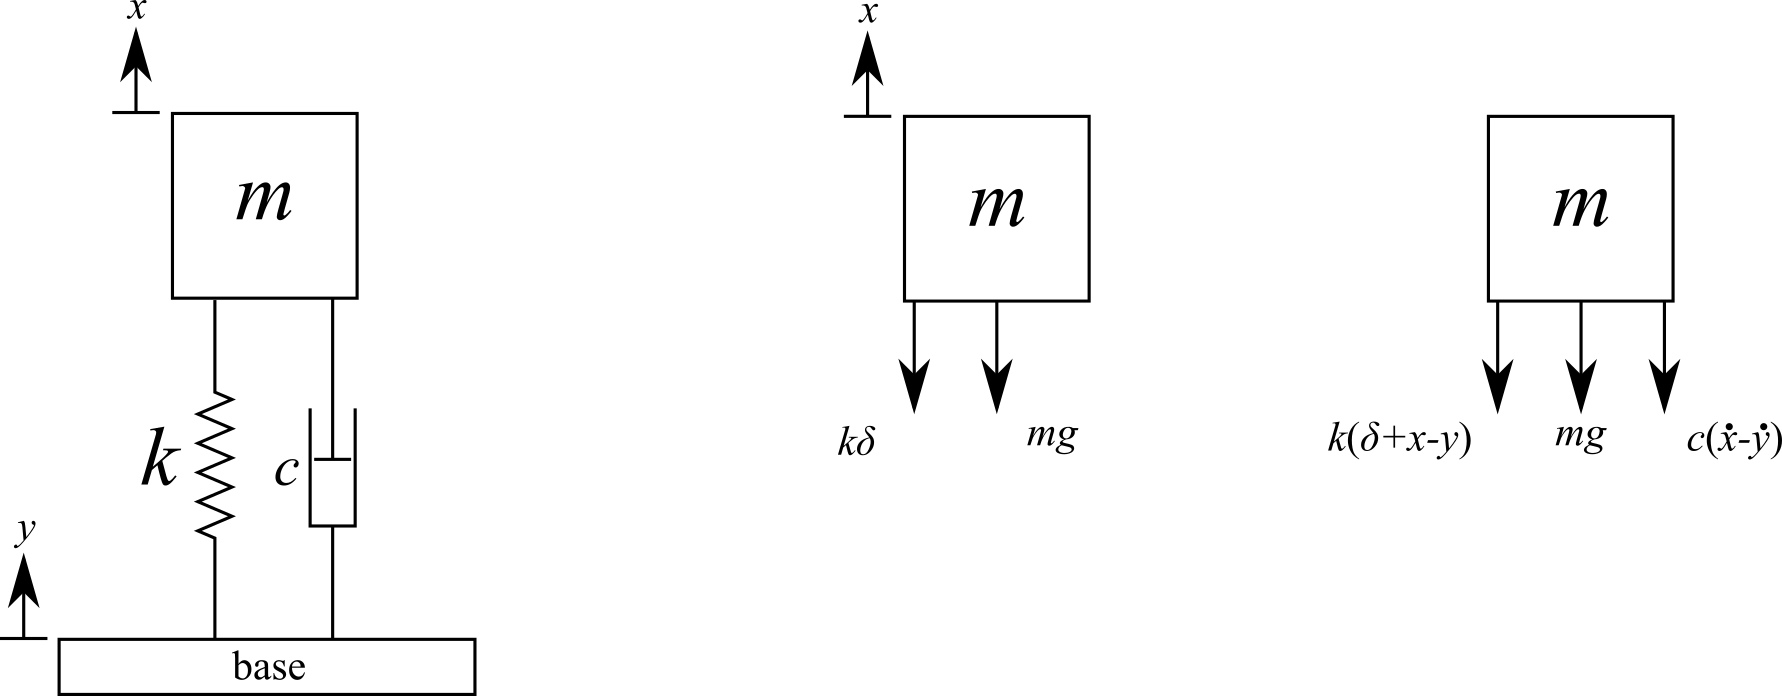
\includegraphics[width=0.8\textwidth]{../Figures/base_excited_1_DOF_model_and_FBDs.png}
\end{figure}
where $x$ is the displacement of the mass and $y$ is the displacement of the base. \textbf{Note that we consider positive upward here.} The EOM can be constructed the same as before, but now considering that the displacement of the springs and damper is $x-y$.  In the equilibrium state, where a positive $x$ is up and the base displaces down:
\begin{equation}
-k\delta -mg =0
\end{equation}	
Note that these are both negative because the base displacing down ``pulls'' the mass down with a force $k\delta$ (i.e. if you hold the mass and let the base ``fall''). Conversely, the equation for the displaced state is:
\begin{equation}
\sum F_x = -k(\delta + x - y) -mg -c(\dot{x} -\dot{y})
\end{equation}	
Apply Newton's second law about the mass ($m\ddot{x}$) of motion to the sum of forces for the displaced position we get:
\begin{equation}
\sum F_x = m\ddot{x} = -k\delta -kx + ky -mg -c\dot{x} +c\dot{y}
\end{equation}	
applying the equation $-k\delta -mg =0$, and rearrange into the EOM yields:	
\begin{equation}
m\ddot{x} + c\dot{x} + kx = c\dot{y} + ky 
\end{equation}
Now as before we assume a solution for the base excitation, for simplicity we assume
\begin{equation}
y(t) = Y\text{sin}(\omega_b t)
\end{equation}
Taking the derivative of the assume solution yields
\begin{equation}
\dot{y}(t) = Y \omega_b \text{cos}(\omega_b t)
\end{equation}
where $Y$ is the amplitude and $\omega_b$ is the frequency of the base excitation. Adding these terms into our EOM yields:
\begin{equation}
m\ddot{x} + c\dot{x} + kx = c Y \omega_b \text{cos}(\omega_b t)  + k Y\text{sin}(\omega_b t)  
\end{equation}
We can get this in standard form if we divide by $m$ and apply the equations for the critical damping ratio and natural frequency:
\begin{equation}
\ddot{x} + 2 \zeta \omega_n \dot{x} + \omega_n^2x = 2 \zeta \omega_n \omega_b Y \text{cos}(\omega_b t)  + \omega_n^2 Y\text{sin}(\omega_b t)  
\end{equation}
This equation can be related to a spring-mass-damper system with two harmonic inputs, one cos and one sin as shown below:
\begin{equation}
\ddot{x} + 2 \zeta \omega_n \dot{x} + \omega_n^2x = C \text{cos}(\omega_b t)  + D \text{sin}(\omega_b t)  
\end{equation}
where C and D are arbitrary coefficients. For simplicity, let us just consider the steady-state solution as this is often of more importance when designing systems for continuous use. Therefore the above equation can be expressed as:
\begin{equation}
\ddot{x} + 2 \zeta \omega_n \dot{x} + \omega_n^2x = C \text{cos}(\omega_b t)  + D \text{sin}(\omega_b t)  = x_p(t) 
\end{equation}
To solve this equation we will use the linearity of the system and solve for a solution that is the sum of two partial solutions. Resulting in:
\begin{equation}
 x_p(t) = 	x_p^{(1)}(t) + 	x_p^{(2)}(t)  
\end{equation}

 Recall that the steady state solution for a harmonically excited spring-mass-damper can be expressed as $x_p(t) = X\text{cos}(\omega_b t - \phi_1)$. Therefore, for a base excited problem, the forcing function can be expressed as the sum of partial solutions:
\begin{equation}
	C \text{cos}(\omega_b t)  + D \text{sin}(\omega_b t)   = x_p(t) = 	x_p^{(1)}(t) + 	x_p^{(2)}(t) 
\end{equation}
where:
\begin{equation}
	x_p^{(1)}(t) = X^{(1)}\text{cos}(\omega_b t - \phi_1)
\end{equation}
\begin{equation}
	x_p^{(2)}(t) = X^{(2)} \text{sin}(\omega_b t - \phi_1)
\end{equation}
Note that $x_p^{(1)}(t)$ uses a cos term while $x_p^{(1)}(t)$ uses a sin term. Both solutions use $\phi_1$ as the damping term as the phase angle is independent of the excitation amplitude and the sin and cos terms account for the difference in phase. Now, for $x_p^{(1)}(t)$, we use the method of undetermined coefficients to obtain a solution for $x_p^{(1)}(t) = X^{(1)}\text{cos}(\omega_b t - \phi_1)$. This can be as simple as setting $2 \zeta \omega_n \omega_b Y$ equal to $f_0$ from the equation for $X$. We can do this because both terms can be considered a ``driving force''. This results in the equation:
\begin{equation}
	x_p^{(1)}(t) = \frac{2 \zeta \omega_n \omega_b Y}{\sqrt{(\omega_n^2 - \omega_b^2)^2 +  (2\zeta \omega_n \omega_b)^2}}  \text{cos}(\omega_b t - \phi_1)
\end{equation}
where 
\begin{equation}
	\phi_1 = \text{tan}^-1\bigg(\frac{2\zeta \omega_n \omega_b}{\omega_n^2 - \omega_b^2}\bigg)
\end{equation}	
Next, the partial solution associated with $x_p^{(2)}(t) = X^{(2)} \text{sin}(\omega_b t - \phi_1)$ can be obtained using the same method of undetermined coefficients. This results in:
\begin{equation}
	x_p^{(2)}(t) = \frac{\omega_n^2 Y}{\sqrt{(\omega_n^2 - \omega_b^2)^2 +  (2\zeta \omega_n \omega_b)^2}}  \text{sin}(\omega_b t - \phi_1)
\end{equation}
now, as both equation have the same argument $(\omega_b t - \phi_1)$, these can be added as:
\begin{equation}
	x_p(t) = 	x_p^{(1)}(t) + 	x_p^{(2)}(t)
\end{equation}
to obtain:
\begin{equation}
	x_p(t) = 	\omega_n Y   \sqrt{\frac{\omega_n^2 + (2 \zeta \omega_b)^2 }{(\omega_n^2 - \omega_b^2)^2 +  (2\zeta \omega_n \omega_b)^2} }  \text{cos}(\omega_bt - \phi_1 - \phi_2)
\end{equation}
and:
\begin{equation}
	\phi_2 = \text{tan}^-1\bigg(\frac{\omega_n}{2\zeta \omega_b}\bigg)
\end{equation}
where $\phi_2$ is added to account for the cos and sin terms being combined. As before, if we want to investigate how a frequency input will affect the response (frequency response) we can substitute substitute 
\begin{equation}
r=\frac{\omega_b}{\omega_n}
\end{equation} 
into the temporal response to obtain:
\begin{equation}
X = Y \sqrt{\frac{1+(2 \zeta r)^2}{(1-r^2)^2 + (2 \zeta r )^2}} 
\end{equation} 
Next, if we divide by $Y$ we can obtain a normalized expression for the displacement:
\begin{equation}
\frac{X}{Y} = \sqrt{\frac{1+(2 \zeta r)^2}{(1-r^2)^2 + (2 \zeta r )^2}} 
\end{equation} 
Plotting this for several critical damping ratios:
\begin{figure}[H]
	\centering
	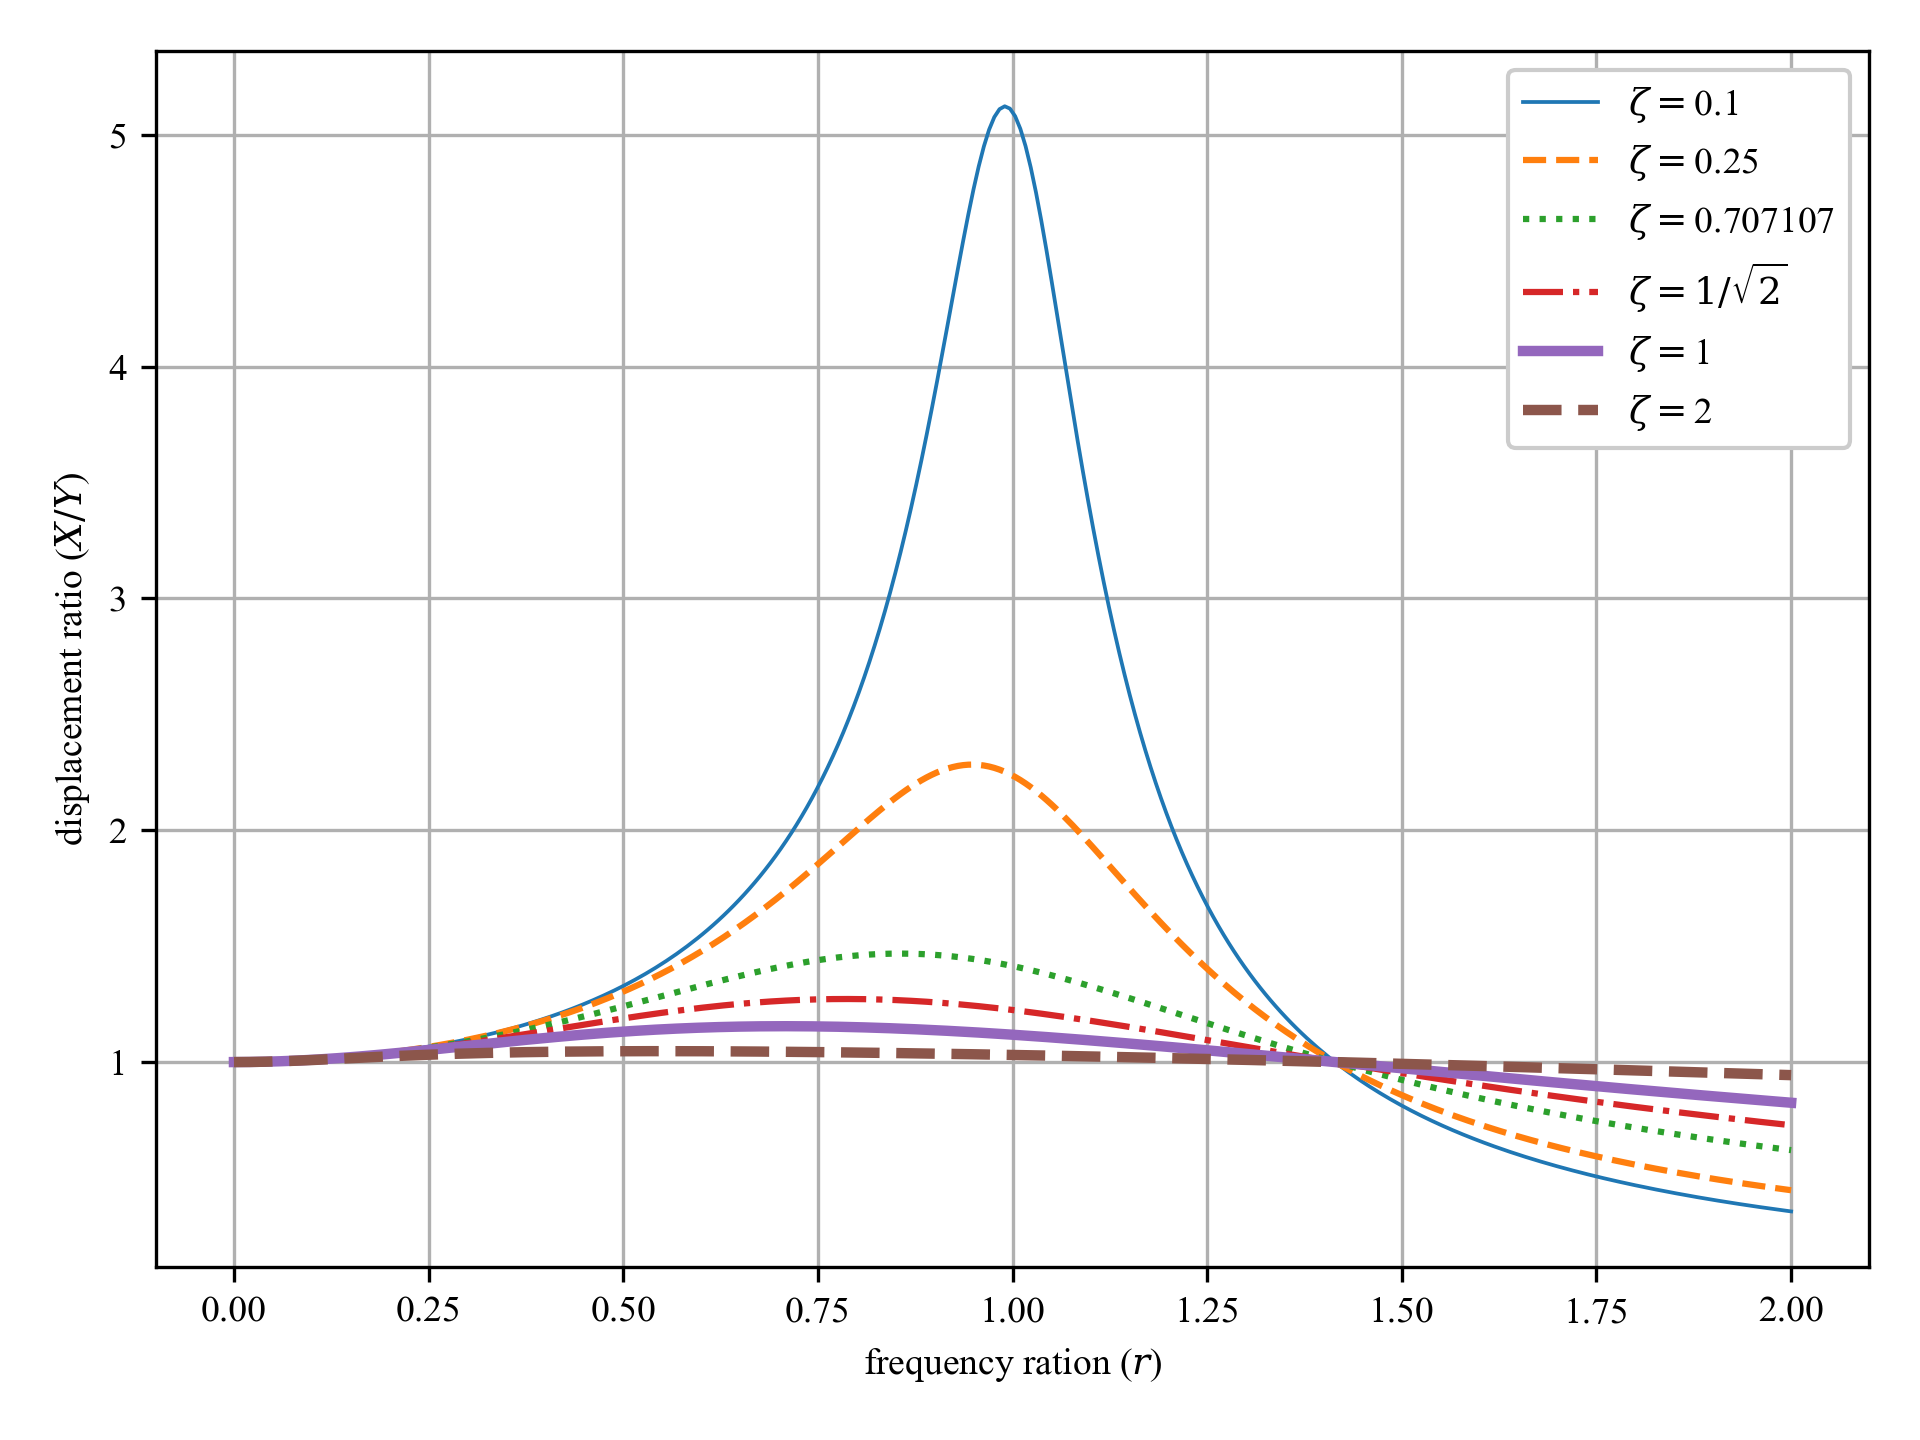
\includegraphics[width=0.8\textwidth]{../Figures/displacement_transmissibility.png}
\end{figure}
Around resonance, the maximum amount of displacement is transmitted to the mass. Additionally,  the above plot shows that at $r=\sqrt{2}$ the displacement transmissibility $X/Y$ is 1. Note the ``flip'' where overdamped systems have a greater response to excitations after $r=\sqrt{2}$ than do underdamped systems.

For some systems, such as those with weak connections, the force transmitted to the mass is more important than the displacement of the mass. The force transmitted to the mass are the sums of the forces applied by the spring and damper. From the FBD above,
\begin{equation}
F(t) = k(x-y) + c(\dot{x} - \dot{y}) 
\end{equation}
where this force is counteracted by the inertial force of the mass:
\begin{equation}
F(t) = -m\ddot{x}(t)
\end{equation}
Only considering the steady state we found that 
\begin{equation}
	x_p(t) = 	\omega_n Y   \sqrt{\frac{\omega_n^2 + (2 \zeta \omega_b)^2 }{(\omega_n^2 - \omega_b^2)^2 +  (2\zeta \omega_n \omega_b)^2} }  \text{cos}(\omega_bt - \phi_1 - \phi_2)
\end{equation} 
if we differentiate this twice, to obtain $\ddot{x}(t)$ and combine this with $F(t) = -m\ddot{x}(t)$ we get:
\begin{equation}
	F(t) = 	m \omega_b^2 \omega_n Y   \sqrt{\frac{\omega_n^2 + (2 \zeta \omega_b)^2 }{(\omega_n^2 - \omega_b^2)^2 +  (2\zeta \omega_n \omega_b)^2} }  \text{cos}(\omega_bt - \phi_1 - \phi_2)
\end{equation} 
Again applying 
\begin{equation}
	r=\frac{\omega_b}{\omega_n}
\end{equation} 
this becomes:
\begin{equation}
	F(t) = 	F_\text{T} \text{cos}(\omega_bt - \phi_1 - \phi_2)
\end{equation} 
where $F_T$ is the magnitude of the transmitted force and is 
\begin{equation}
	F_\text{T} = kYr^2 \sqrt{\frac{1+(2 \zeta r)^2}{(1-r^2)^2 + (2 \zeta r )^2}} 
\end{equation}
Again, this can be converted to a force transmissibility to provide a normalized response such that:
\begin{equation}
	\frac{F_\text{T}}{kY} = r^2 \sqrt{\frac{1+(2 \zeta r)^2}{(1-r^2)^2 + (2 \zeta r )^2}} 
\end{equation}
Plotting this for several critical damping ratios:
\begin{figure}[H]
	\centering
	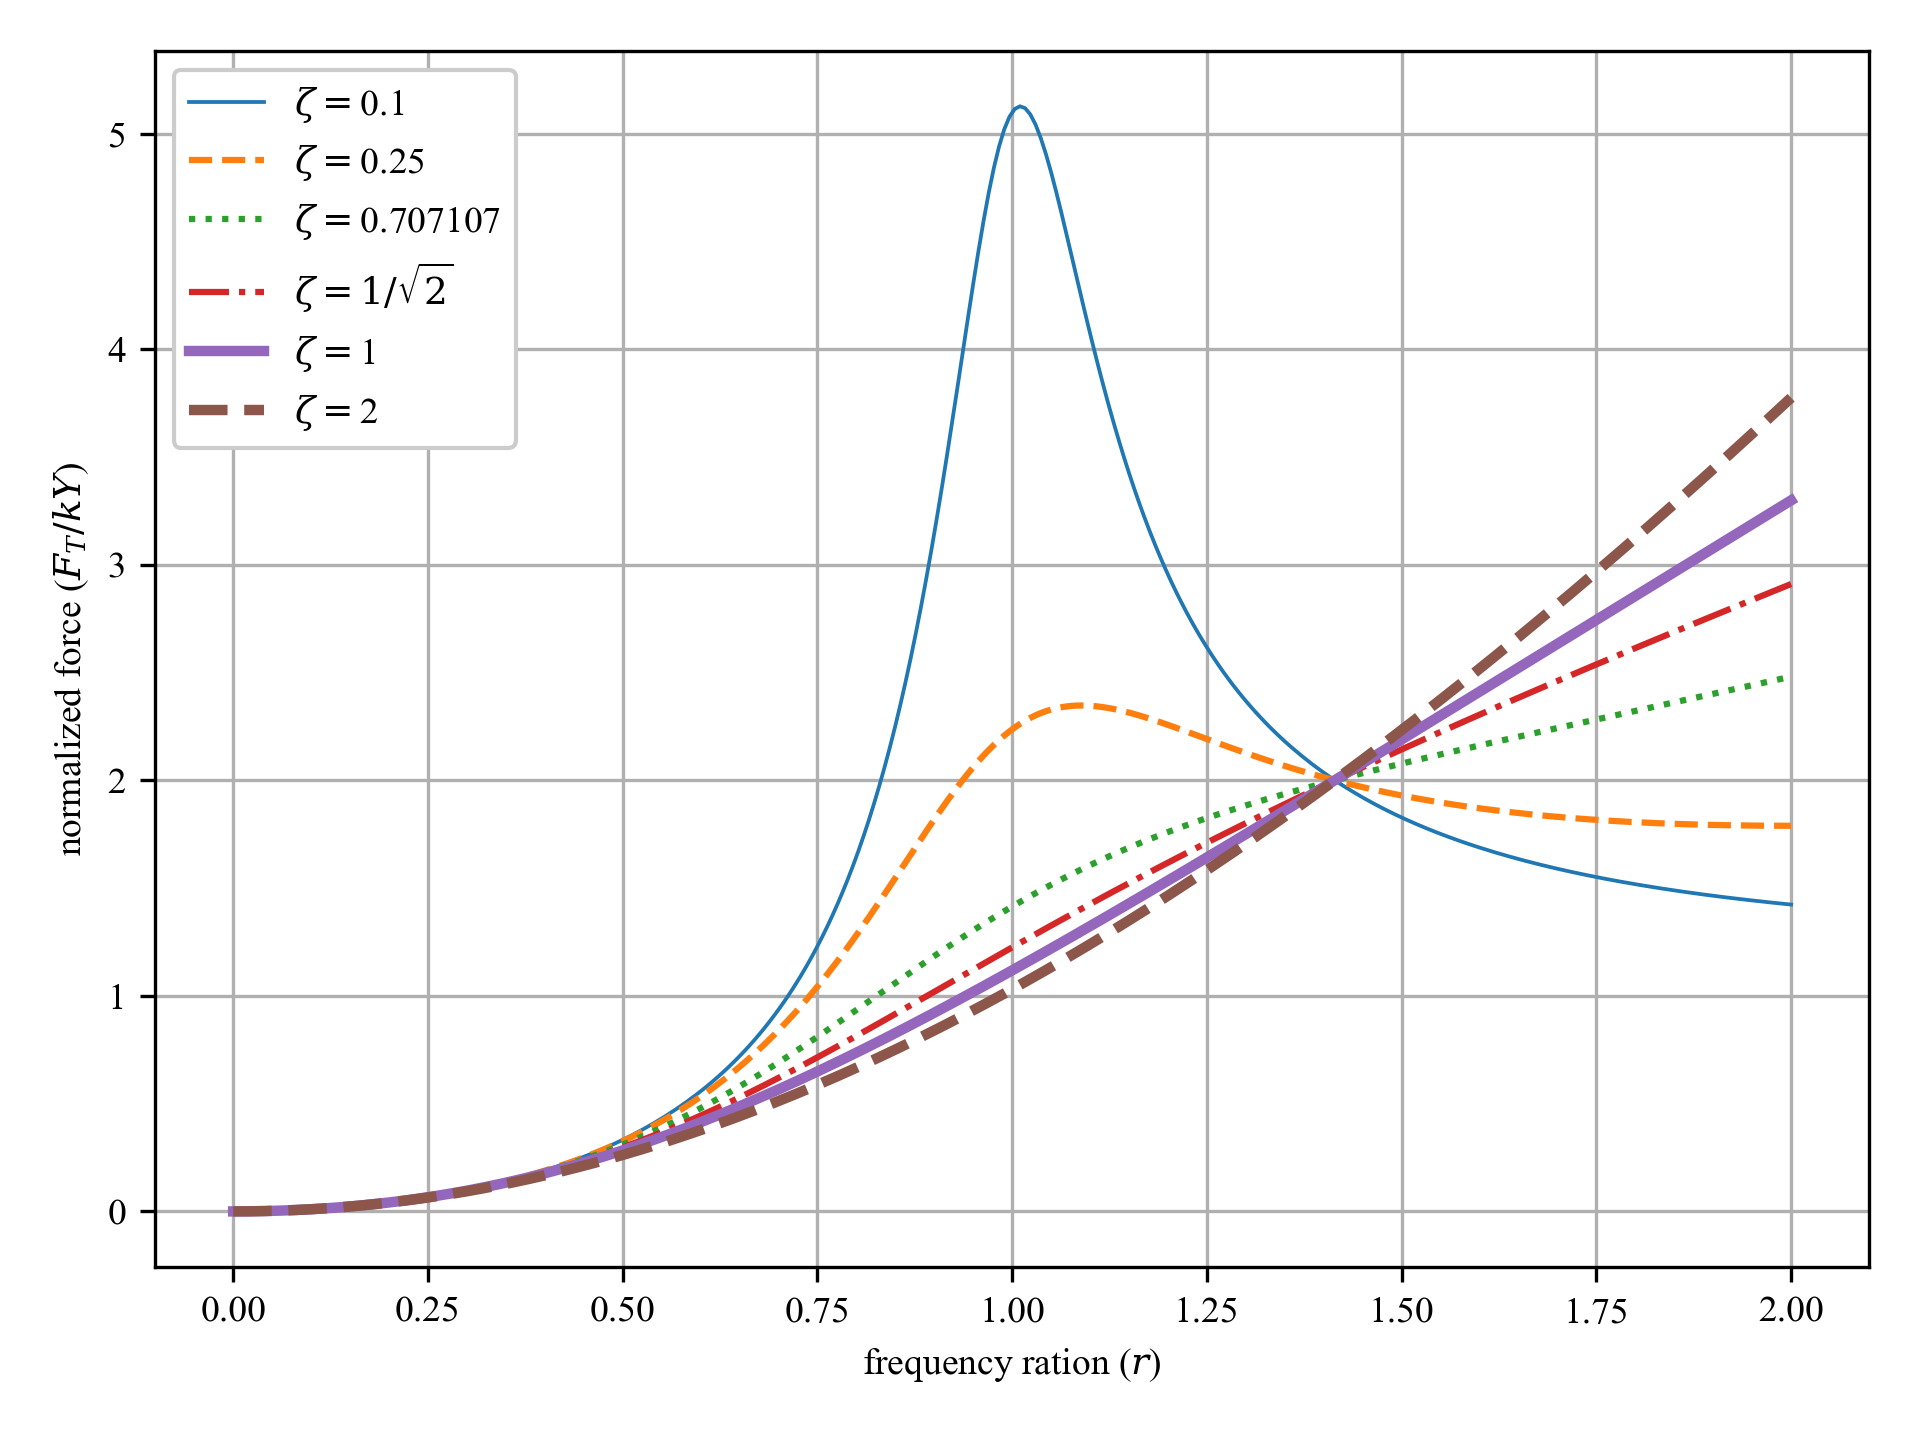
\includegraphics[width=0.8\textwidth]{../Figures/force_transmissibility.png}
\end{figure}
Again, note the key location $r=\sqrt{2}$. At $r=\sqrt{2}$ the force transmitted to the system is 2 $\frac{F_\text{T}}{kY}$. However, also note that the normalized force does not necessarily fall off for $r$ values greater than $r=\sqrt{2}$.  

\begin{example}


			For a given system 1-DOF excited at the base should the system be excited above or below the natural frequency if the transmitted force is the design limitation? Consider the under damped with $\zeta=0.1$, and the over damped with $\zeta=2$ conditions. 

			\textbf{Solution}
			
			We can plot the transmissibility of both the force and displacement onto one plot. For $\zeta=0.1$
			\begin{figure}[H]
				\centering
				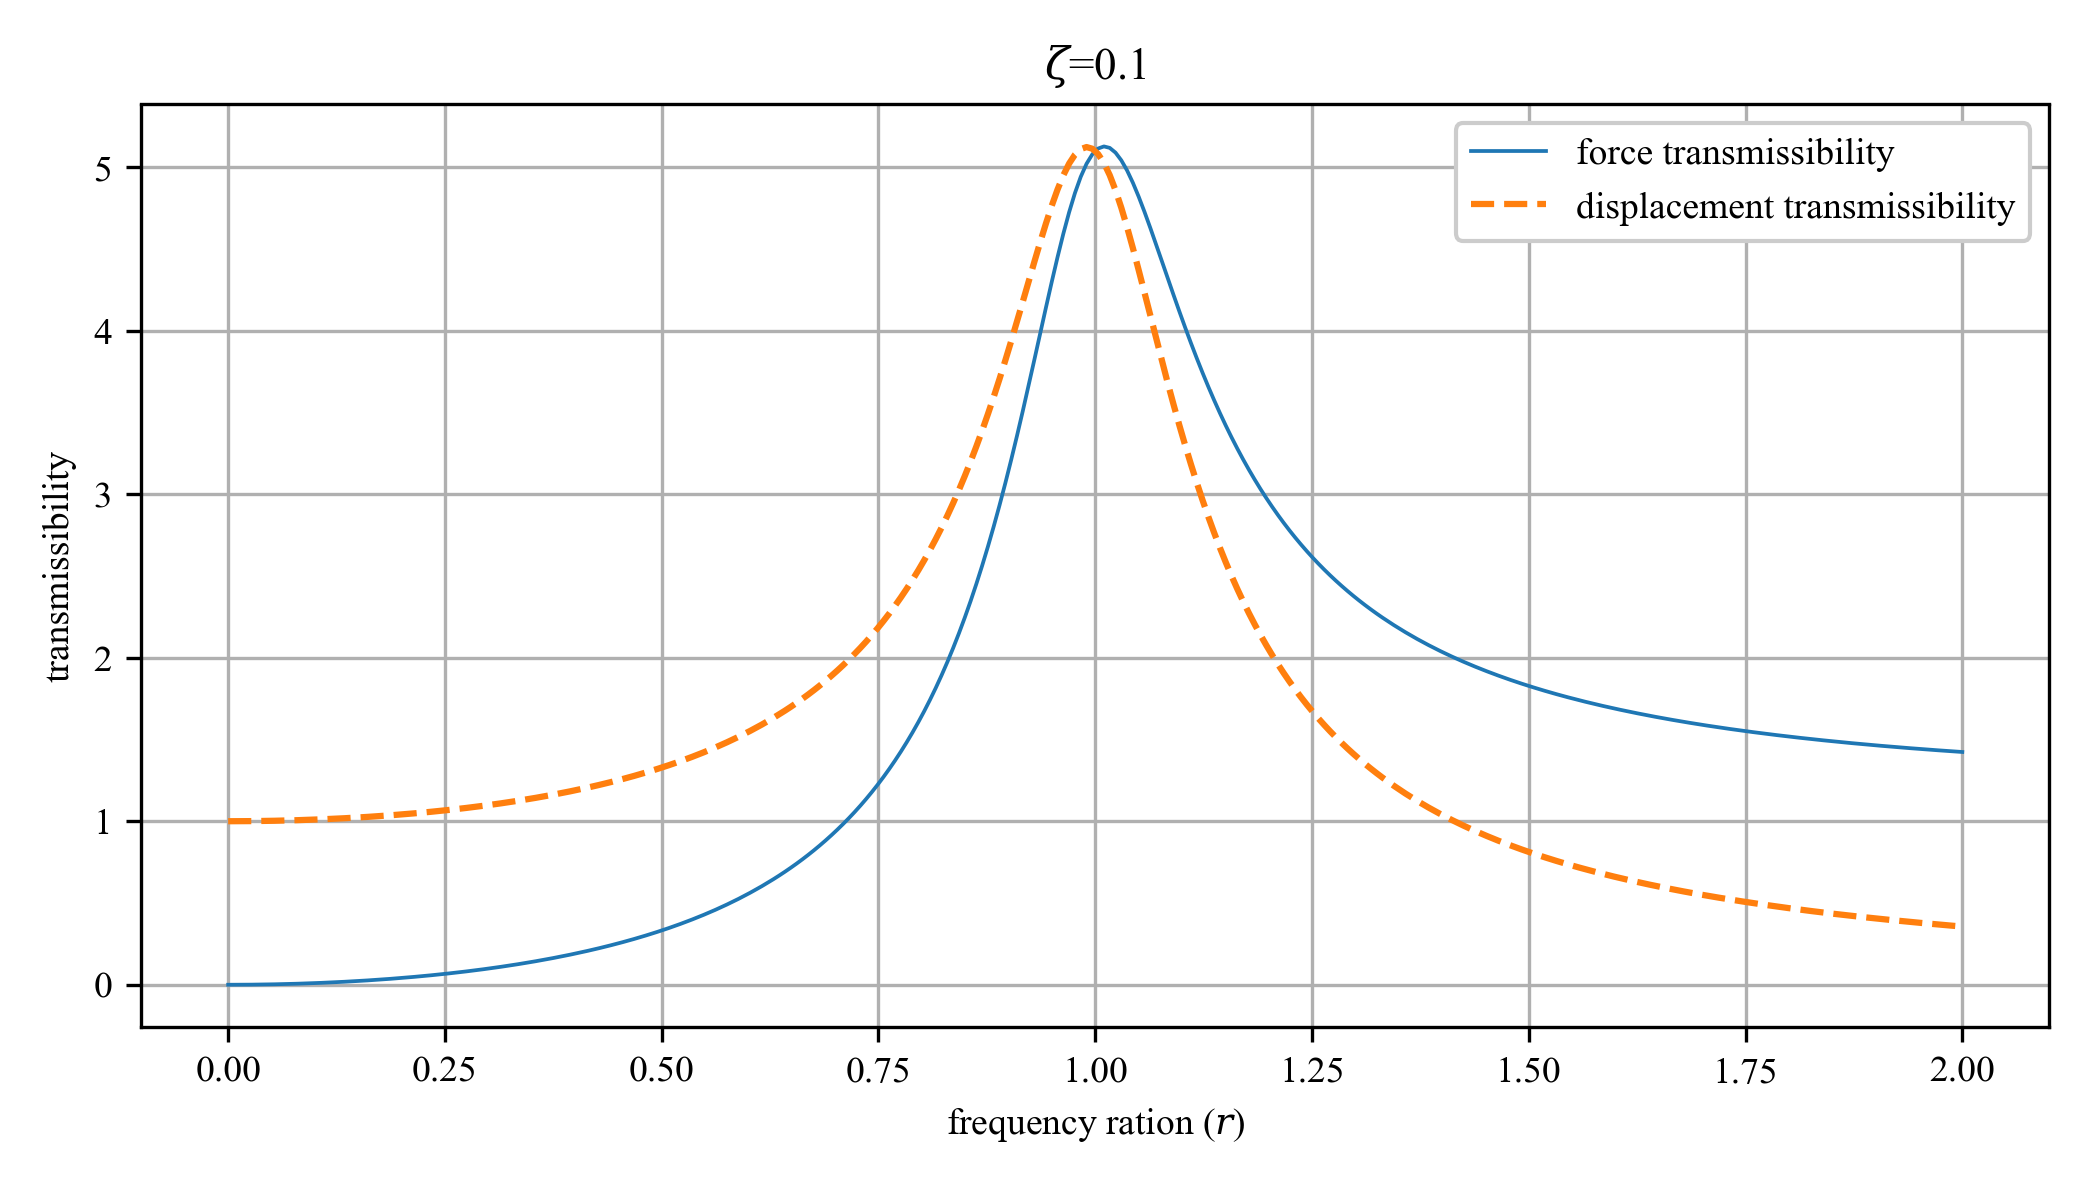
\includegraphics[width=0.8\textwidth]{../Figures/example_1_force_displacement_transmissibility_1.png}
			\end{figure}
			it is clear that to minimize the force, the system should be driven with a frequency below the natural frequency. Next for  $\zeta=2$
			\begin{figure}[H]
				\centering
				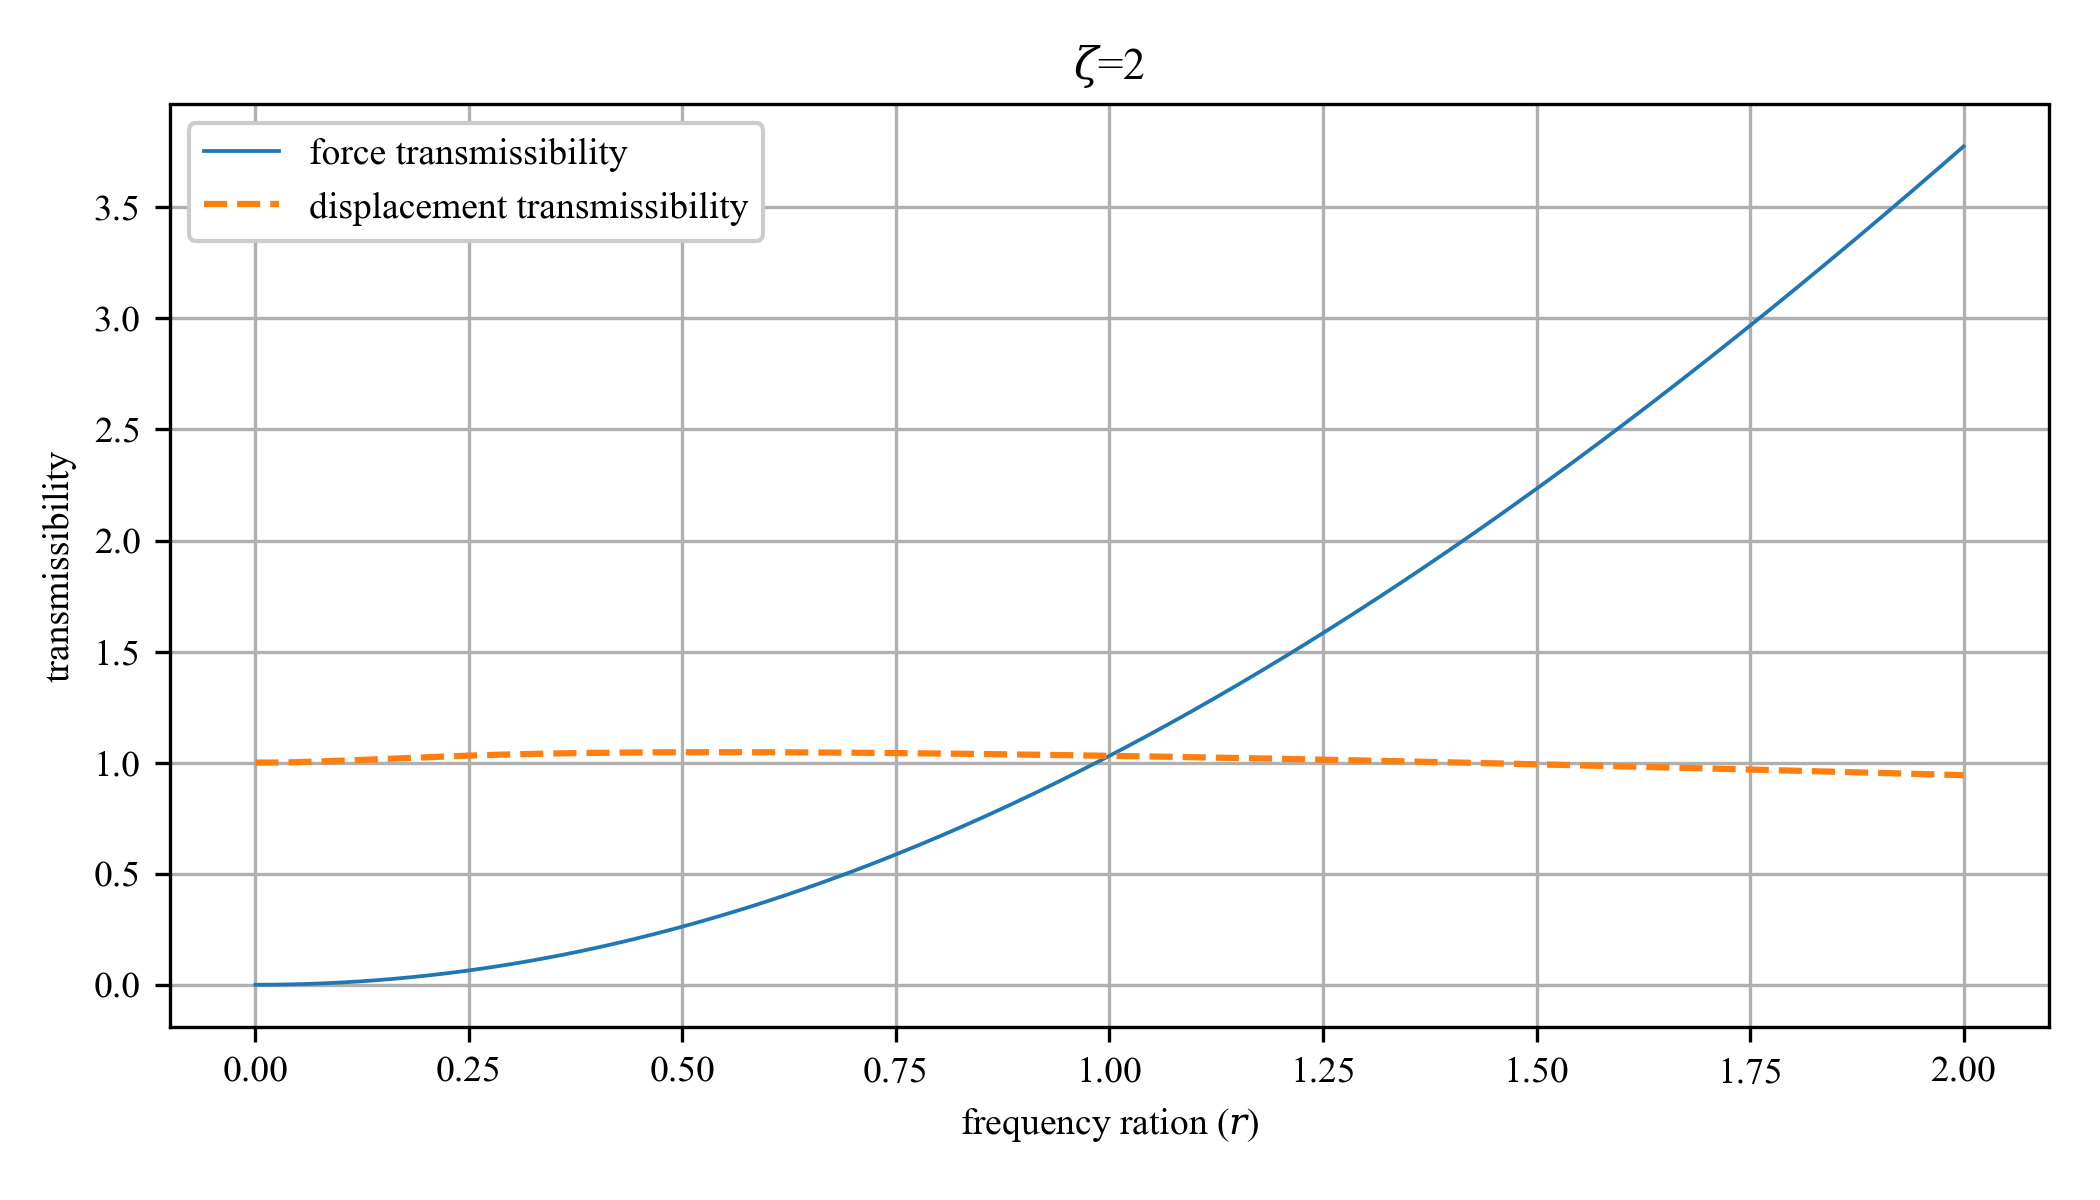
\includegraphics[width=0.8\textwidth]{../Figures/example_1_force_displacement_transmissibility_2.png}
			\end{figure}			
			it can be seen that the same rationale applies. 

\end{example}

\begin{example}

			A \textbf{very common} example of base motion is the SDOF model of a vehicle wheel driving over a ``rough'' road as shown below. 
			\begin{figure}[H]
				\centering
				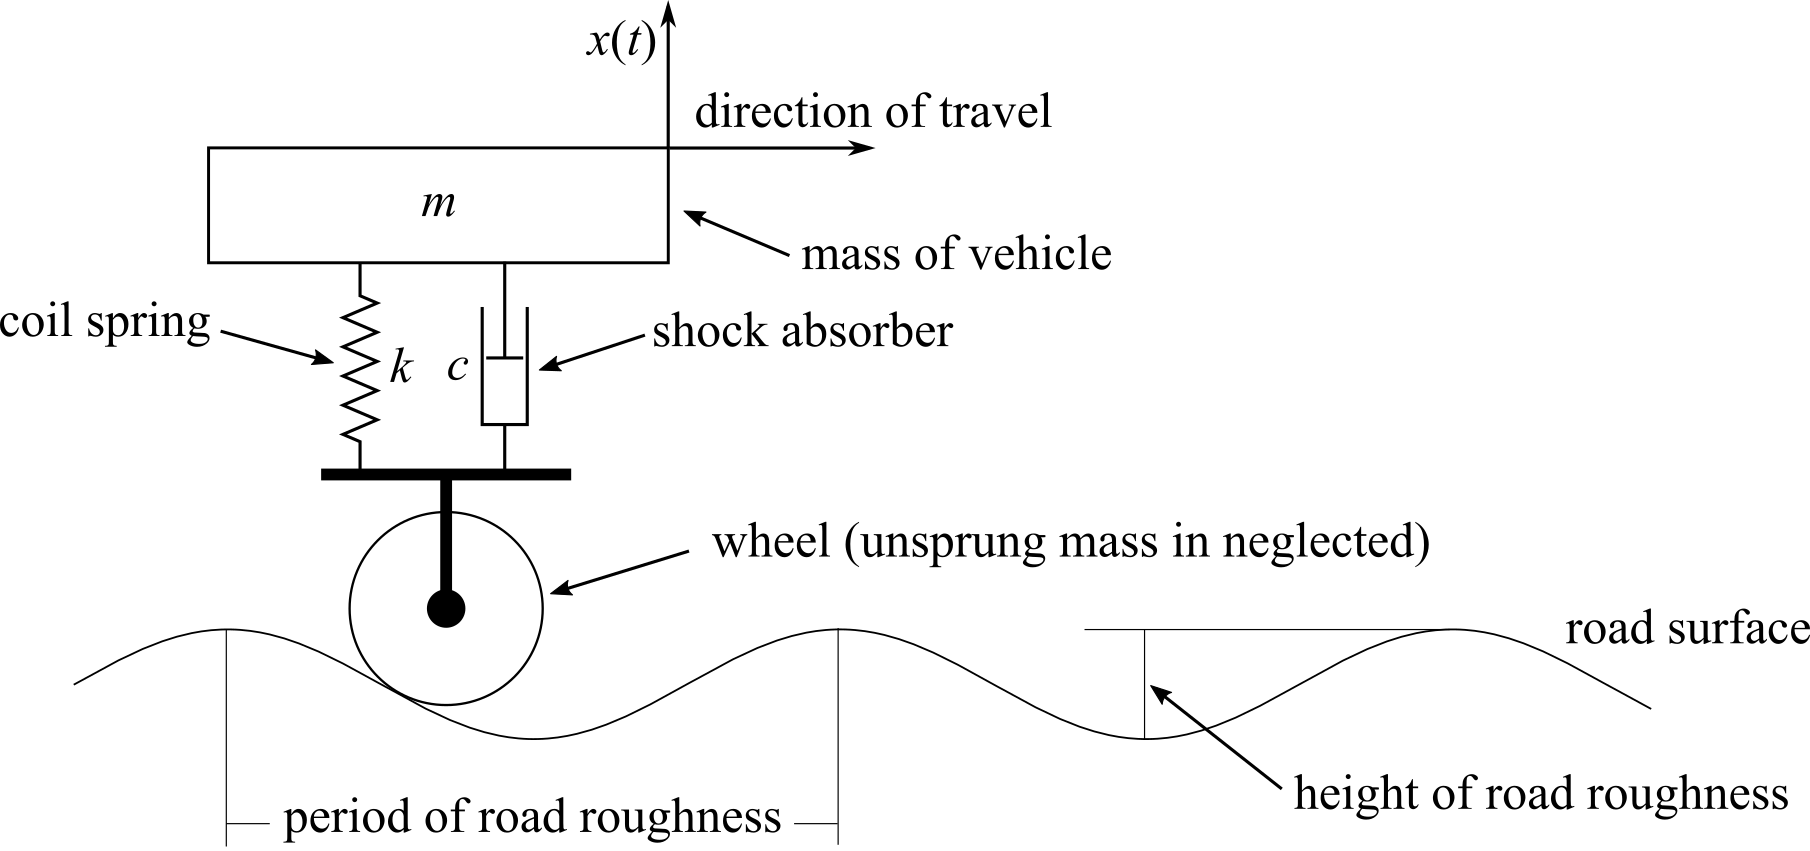
\includegraphics[]{../Figures/Vehicle_on_road_example.png}
			\end{figure}				
			where $k$ = 400,000 N, $m$ = 1007 kg, $c$ = 20,000 kg/s, the period of road roughness = 6m, and eight of road roughness = 0.02 m. What is the defection experience by the car at $v$ = 20 km/h?
			
			\textbf{Solution}

			The road is applying a base excitation that can be approximated as 
			\begin{equation}
				Y = 0.01 \text{ m}
			\end{equation} 				
			\begin{equation}
				v \text{ m/s} = 20 \text{ km/hr}\Bigg(\frac{1000 \text{ m}}{1 \text {km}}\Bigg) \Bigg(\frac{1 \text{ hours}}{3600 \text { s}}\Bigg) = \frac{50}{9} \text{ m/s} = 5.555 \text{ m/sec}
			\end{equation} 	
			\begin{equation}
				\omega_b = \Bigg(\frac{ 5.55 \text{ m}}{s}\Bigg) \Bigg(\frac{ 1 \text{ cycle}}{6 \text{ m}}\Bigg) \Bigg(\frac{ 2 \pi \text{ rad}}{\text {cycle}}\Bigg) = \frac{ 11.11 \pi }{6 } \text{ rad/s} =5.817 \text{ rad/s} 
			\end{equation} 	
			Therefore, the sinusoidal for the base excitation is then:
			\begin{equation}
				y(t) = (0.01) \text{sin}(5.817 t)
			\end{equation} 	
			Next, we can calculate the natural frequency:
			\begin{equation}
				\omega_n = \sqrt{\frac{k}{m}} = \sqrt{\frac{400,000}{1007}} = 19.93 \text{ rad/s}
			\end{equation} 			
			Therefore:
			\begin{equation}
			r=\frac{\omega_b}{\omega_n} = \frac{5.817}{19.93} =0.292
			\end{equation} 		
			and:
			\begin{equation}
			\zeta = \frac{c}{2\sqrt{km}}= \frac{20,000}{2\sqrt{1007\cdot400,000}} = 0.498
			\end{equation}	
			Then it can be found that the maximum deflection of the car is:
			into the temporal response to obtain:
			\begin{equation}
			X = Y \sqrt{\frac{1+(2 \zeta r)^2}{(1-r^2)^2 + (2 \zeta r )^2}} = Y \sqrt{\frac{1+(2 \cdot 0.498 \cdot 0.292)^2}{(1-0.292^2)^2 + (2 \cdot 0.498 \cdot 0.292 )^2}}  = 0.0108 \text{ m}
			\end{equation} 		
\end{example}				
			
\begin{example}
	
			A single story building is subjected to a harmonic ground motion, $\ddot{y}(t) = A \text{cos}(\omega_b t)$. a) Find the steady-state solution for the structure.  b) If a damper was added between the base and the floor, and $r=2$, what would be the ideal critical damping coefficient to insure the safety of the building. (Think of safety as limiting displacement and transmitted force.) 
			\begin{figure}[H]
				\centering
				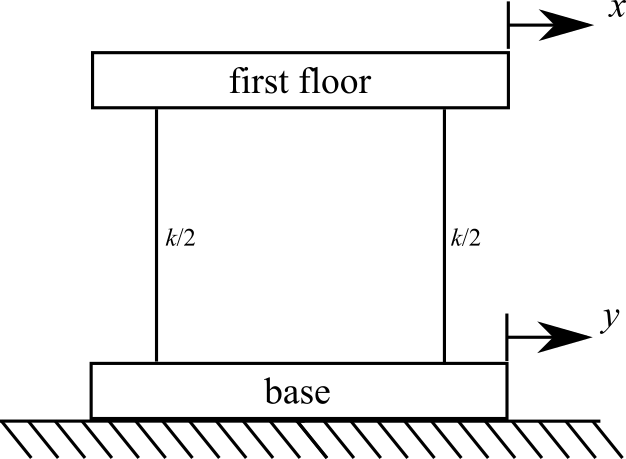
\includegraphics[width=0.35\textwidth]{../Figures/base_excited_structure.png}
			\end{figure}				
						
			\textbf{Solution a)}
				
			For simplicity, we can rearrange the system as what follows:
			\begin{figure}[H]
				\centering
				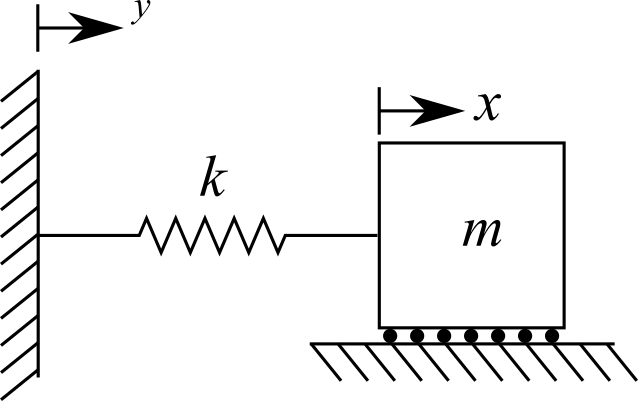
\includegraphics[width=0.35\textwidth]{../Figures/base_excited_structure_simple.png}
			\end{figure}			

			solving for the EOM yields:
			\begin{equation}
				m\ddot{x} + kx = ky
			\end{equation} 				
			Notice that this is the same as the EOM for a damped 1-DOF system if $c=0$.	
			\begin{equation}
			m\ddot{x} + c\dot{x} + kx = + c\dot{y} + ky \rightarrow m\ddot{x} + kx = ky
			\end{equation}
			Therefore, we can use the solution:
			\begin{equation}
				x_p(t) = 	\omega_n Y   \sqrt{\frac{\omega_n^2 + (2 \zeta \omega_b)^2 }{(\omega_n^2 - \omega_b^2)^2 +  (2\zeta \omega_n \omega_b)^2} }  \text{cos}(\omega_bt - \phi_1 - \phi_2)
			\end{equation}
			where:
			\begin{equation}
				\phi_1 = \text{tan}^-1\bigg(\frac{2\zeta \omega_n \omega_b}{\omega_n^2 - \omega_b^2}\bigg)
			\end{equation}	
			\begin{equation}
				\phi_2 = \text{tan}^-1\bigg(\frac{\omega_n}{2\zeta \omega_b}\bigg)
			\end{equation}
			Now we have, or can easily get, values for $\omega_n$, $\omega_b$, and $\zeta$. However, we do not have an expression for $Y$. We can extract the displacement (and therefore the $Y$) from the acceleration as:
			\begin{equation}
				\ddot{y}(t) = A \text{cos}(\omega t)
			\end{equation} 				
			\begin{equation}
				\dot{y}(t) = \frac{A}{\omega} \text{sin}(\omega t) + C_1
			\end{equation} 					
			\begin{equation}
				y(t) = - \frac{A}{\omega^2} \text{cos}(\omega t) + C_1t + C_2
			\end{equation} 					
			Resulting in 
			\begin{equation}
				Y = -\frac{A}{\omega^2}
			\end{equation} 			
			
			\textbf{Solution b)}
			From the plots we solved for before, we can see that we want a critical damping coefficient that is as low as possible. This means any damping added to the system will decrease its safety. This may seem counter-intuitive, but this is because we are attempting to drive the structure at a frequency higher than its natural frequency, something that does not commonalty happen. Typically excitations for a structure are well below its natural frequency.  			
			
\end{example}			
	

		\subsection{Transfer Function method (Generic)}

Consider the following system
\begin{figure}[H]
	\centering
	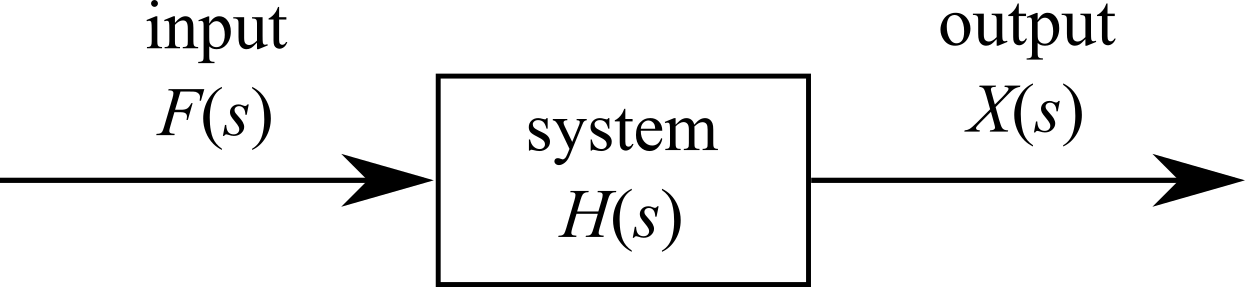
\includegraphics[width=0.5\textwidth]{../Figures/system_input_output.png}
\end{figure}
where $F(s)$ is the input, $H(s)$ is the system, and $X(s)$ is the output from the system. This formulation is called the transfer-function approach and is commonly used for the formulation and solution of dynamic problems in the control literature. It can also be used for solving the various forced-vibration problems including those from complex or stochastic inputs. 

Examples of force excitation that can be calculated include using this method include:
\begin{itemize}
	\item sinusoidal
	\item base excitation
	\item impulse
	\item arbitrary input
	\item arbitrary periodic input
\end{itemize}

		\subsubsection{Review of Laplace Transforms}
		
		 An integral transform is the procedure of integrating the time dependence of a function into becoming a function of an alternative variable, or parameter, which can be manipulated algebraically. 
		
		Of interest to this class is the Laplace transform ($\Laplace{f(t)}$) of the function $f(t)$. Here, a Laplace transform is used as a method of solving the differential equations of motion by reducing the computation needed to that of integration and algebraic manipulation. 
		
		The definition of the Laplace transform of the function $f(t)$ is:
		
		\begin{equation}
				\Laplace{f(t)} = F(s) = \int_{0}^{\infty} f(t)e^{-st}dt
		\end{equation}
		where $f(t)=0$ for all values of $t$ less than 0. Here, the $s$ is a complex value. Lastly, the term $F(s)$is a generic term that  represents the input to a system. As this class needs the derivative of functions, we will calculate that next:
		\begin{equation}
			\Laplace{\dot{f}(t)} = \int_{0}^{\infty} \dot{f}(t)e^{-st}dt = \int_{0}^{\infty} e^{-st}\frac{d[f(t)]}{dt}dt 
		\end{equation}		
		integration by parts yields
		\begin{equation}
			\Laplace{\dot{f}(t)} = e^{-st}f(t)\Big|_0^\infty+s\int_{0}^{\infty}e^{-st}f(t)dt
		\end{equation}
		Astutely, it can be noticed that the second term $s\int_{0}^{\infty}e^{-st}f(t)dt$
		is the input to the system $F(s)$. Therefor, with a little rearranging this becomes:
		\begin{equation}
			\Laplace{\dot{f}(t)} = sF(s)-f(0)
		\end{equation}
		Successive iteration yields:
		\begin{equation}
			\Laplace{\ddot{f}(t)} = s^2F(s)-sf(0)-\dot{f}(0)
		\end{equation}
		
		A few key points of the Laplace transforms are:
		
		
		\begin{itemize}
			\item the domain of the problem from the real number line ($t$) to the complex plane ($s$).
			\item The integration of the Laplace transform changes differentiation into multiplication.
			\item The transform procedure is linear. Therefore, the transform of the linear combination of two transforms is the same as the linear transformation of these functions. 
			\item to move from the time domain to the complex number plane we typically use tables of pre-solved integral. 
			\item The function $x(t)$ can be obtained by taking the inverse Laplace transform defined as $x(t) = \Laplace{X(s)}^{-1}$
		\end{itemize}
		
		The Laplace transform can be calculated in symbolic form. In particular interest to this class is the Laplace form of the system output $X(s)$

		\begin{equation}
			\Laplace{x(t)} = X(s)
		\end{equation}		
		\begin{equation}
			\Laplace{\dot{x}(t)} = sX(s)-x(0)
		\end{equation}	
		\begin{equation}
			\Laplace{\ddot{x}(t)} = s^2X(s)-sx(0) - \dot{x}(0)
		\end{equation}	
		here, $x(0)$ and $\dot{x}(0)$ are the initial values of the function $x(t)$. 
		


The procedure for using the Laplace transform to solve equations of motion expressed as an inhomogeneous ordinary differential equation is:
\begin{enumerate}
	\item Take the Laplace transform of both sides of the EOM while treating the time derivatives symbolically.
	\item Solve for $X(s)$ in the obtained equation.
	\item Apply the inverse transform $x(t) = \Laplace{X(s)}^{-1}$
\end{enumerate}

\subsubsection{Transfer Function method (homogeneous differential equation)}

Consider the undamped single-DOF system:
\begin{figure}[H]
	\centering
	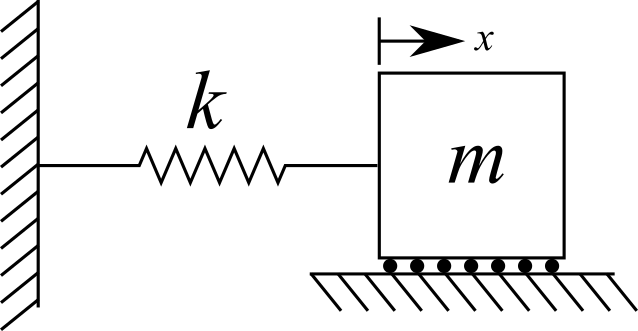
\includegraphics[width=0.4\textwidth]{../Figures/1-DOF-mass_horizontal.png}
\end{figure}
that can be described the the EOM in standard form:
\begin{equation}
	\ddot{x}(t) + \omega_n^2x(t) = 0 
\end{equation}
where the initial conditions are $x(0)=x_0$ and $\dot{x}(0) = v_0$. Taking the Laplace transforms of both sides of the EOM yields:
\begin{equation}
	\ddot{x}(t)  = s^2X(s) -sx_0 -v_0
\end{equation}
\begin{equation}
	\omega_n^2x(t) = \omega_n^2X(s)
\end{equation}
resulting in:
\begin{equation}
	s^2X(s) -sx_0 -v_0 + \omega_n^2X(s) = 0
\end{equation}
solving for the output of the system $X(s)$ yields:
\begin{equation}
X(s) = \frac{sx_0 + v_0}{s^2 + \omega_n^2}
\end{equation}
We can expand this form of $X(s)$ to obtain equations listed in our Laplace Transform table:
\begin{equation}
X(s) = \frac{sx_0}{s^2 + \omega_n^2} + \frac{v_0}{s^2 + \omega_n^2}\cdot \frac{\omega_n}{\omega_n}
\end{equation}
This becomes:
\begin{equation}
X(s) = x_0\frac{s}{s^2 + \omega_n^2} + \bigg(\frac{v_0}{\omega_n}\bigg) \cdot \frac{\omega_n}{s^2 + \omega_n^2}\cdot 
\end{equation}

Next, using the inverse Laplace transform $x(t) = \Laplace{X(s)}^{-1}]$ and the two following Laplace transforms (\#5 and \#6):
\begin{equation}
f(t) \text{ is cos}(\omega t) \text{ when }  F(s) \text{ is } \frac{s}{s^2+\omega^2} 
\end{equation}
\begin{equation}
f(t) \text{ is sin}(\omega t)  \text{ when }  F(s) \text{ is } \frac{\omega}{s^2+\omega^2} 
\end{equation}
Therefore, we can obtain the solution for the system output $X(s)$ as:
\begin{equation}
x(t) = x_0 \text{cos}(\omega_n t) + \frac{v_0}{\omega_n}\text{sin}(\omega_n t)
\end{equation}

The same procedure works for calculating the under damped and forced responses, however, in these responses calculating the algebraic solution for $X(s)$ often results in quotients of polynomials in $s$. These Polynomial ratios may not be found in simple Laplace tables and must be solved using the \textbf{method of partial fractions}. An example of this procedure can be found in Appendix B of Inman. 

%\textbf{Example 2}
%Consider the system:
%\begin{figure}[H]
%	\centering
%	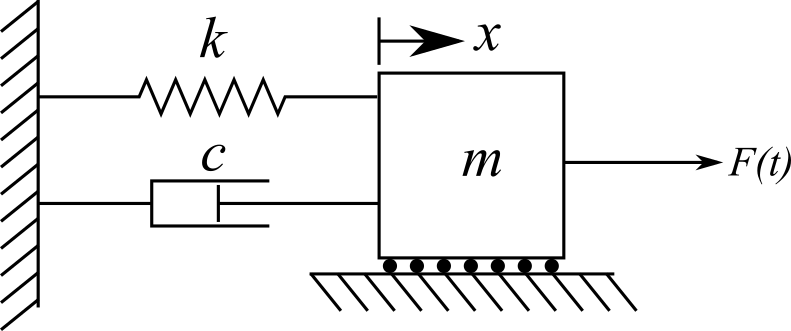
\includegraphics[width=0.4\textwidth]{../Figures/forced_spring_mass_damper_system.png}
%\end{figure}
%that can be described the the EOM in standard form:
%\begin{equation}
%\ddot{x}(t) + 2 \zeta \omega_n \dot{x}+ \omega_n^2x(t) = 0 \text{, where }x(0)=x_0 \text{, and } \dot{x}(0) = v_0 
%\end{equation}
%Taking the Laplace transform of both sides of the EOM yields:
%\begin{equation}
%\big(s^2X(s) -sx_0 -v_0\big)+\big(s2 \zeta \omega_n X(s)-x_0\big)+\big(\omega_n^2X(s)\big) = 0
%\end{equation}
%considering that $sx_0 + x_0$ can be expressed as $sx_0$ because they are both based on the initial condition $x_0$. solving for the output of the system $X(s)$ yields:
%\begin{equation}
%X(s) = \frac{sx_0 + v_0}{s^2 + 2 \zeta \omega_n s+ \omega_n^2}
%\end{equation}
%Using the method of partial fractions, this can be expressed as inverse Laplace transform $x(t) = \Laplace{X(s)}^{-1}$ resulting in:
%\begin{equation}
%F(s) \text{ is } \frac{1}{s^2 + 2 \zeta \omega s+ \omega^2} \text{ when } f(t) \text{ is}\frac{1}{\omega_d}e^{-\zeta \omega t}\text{sin}(\omega_n t),
%\end{equation}
%\begin{equation}
%\text{when } \zeta < 1\text{, and } \omega_d = \sqrt{1-\zeta^2} \nonumber
%\end{equation}
%Therefore, we can obtain the solution for the system output $X(s)$ as:
%\begin{equation}
%x(t) = x_0 \text{cos}(\omega_n t) + \frac{v_0}{\omega_n}\text{sin}(\omega_n t)
%\end{equation}

\subsubsection{Impulse Response Function}
A very common source of vibration is the sudden application for a short-duration force called an impulse. An impulse excitation is a force that is applied for a very short, or infinitesimal, length of time and represents one example of a shock loading. An impulse is a nonperiodic force that is represented by the symbol $\delta$. The response of a system to an impulse is identical to the free response of the system to certain initial conditions.This is illustrated in the following, in many useful situations the applied force $F(t)$ is impulsive in nature
(i.e., acts with large magnitude for a very short period of time).

\begin{figure}[H]
	\centering
	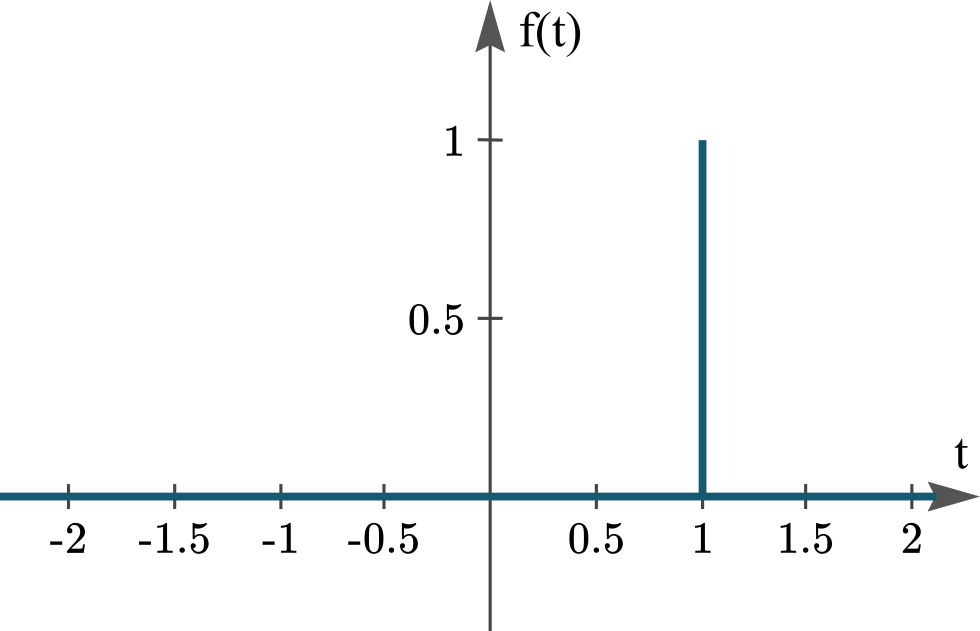
\includegraphics[width=0.5\textwidth]{../Figures/impulse_time_history.png}
\end{figure}

The impulse response function can be solved for analytically, however, we will solve it using the transfer function approach. Here we will consider the under-damped spring-mass system. First, assume that the system is at rest (no initial conditions). Next, we write the EOM as:
\begin{equation}
m\ddot{x} +c\dot{x} +kx = \delta(t)
\end{equation}
Taking the Laplace transform of both sides of the equation yields 
\begin{equation}
m\big(s^2X(s)-sx(0) - \dot{x}(0)\big) + c\big(sX(s)-x(0)\big) +kX(s) =1
\end{equation}
However, \textbf{if we assume zero initial conditions} (a system at rest when the impulse happens), the equation simplifies to. 
\begin{equation}
ms^2X(s) + csX(s) +kX(s) =1
\end{equation}
or
\begin{equation}
(ms^2 + cs +k)X(s) =1
\end{equation}
note that the $\Laplace{\delta}=1$ per \#1 in the transform table. Solving this equation for $X(s)$:
\begin{equation}
X(s) = \frac{1}{m} \cdot \frac{1}{s^2 + 2 \zeta \omega_n s + \omega_n^2}
\end{equation}
Again, the mass is extracted to develop a formulation that can be found in the Laplace tables. Setting the constraint that $\zeta<1$ and consulting \#10 in the table for Laplace transforms results in:
\begin{equation}
x(t) = \frac{1}{m \omega_d} e^{-\zeta \omega_n t} \text{sin}(\omega_dt)
\end{equation}
where this is the general solution for a damped system subjected to an impulse loading function. For the undamped case a solution can be obtained by setting $\zeta=0$. This Results in the following form for the undamped case:
\begin{equation}
x(t) = \frac{1}{m \omega_n}\text{sin}(\omega_n t)
\end{equation}
Below is a typical response for both a undamped and underdamped 1-DOF system subject to an impulse response at $t=0$ seconds. 
\begin{figure}[H]
	\centering
	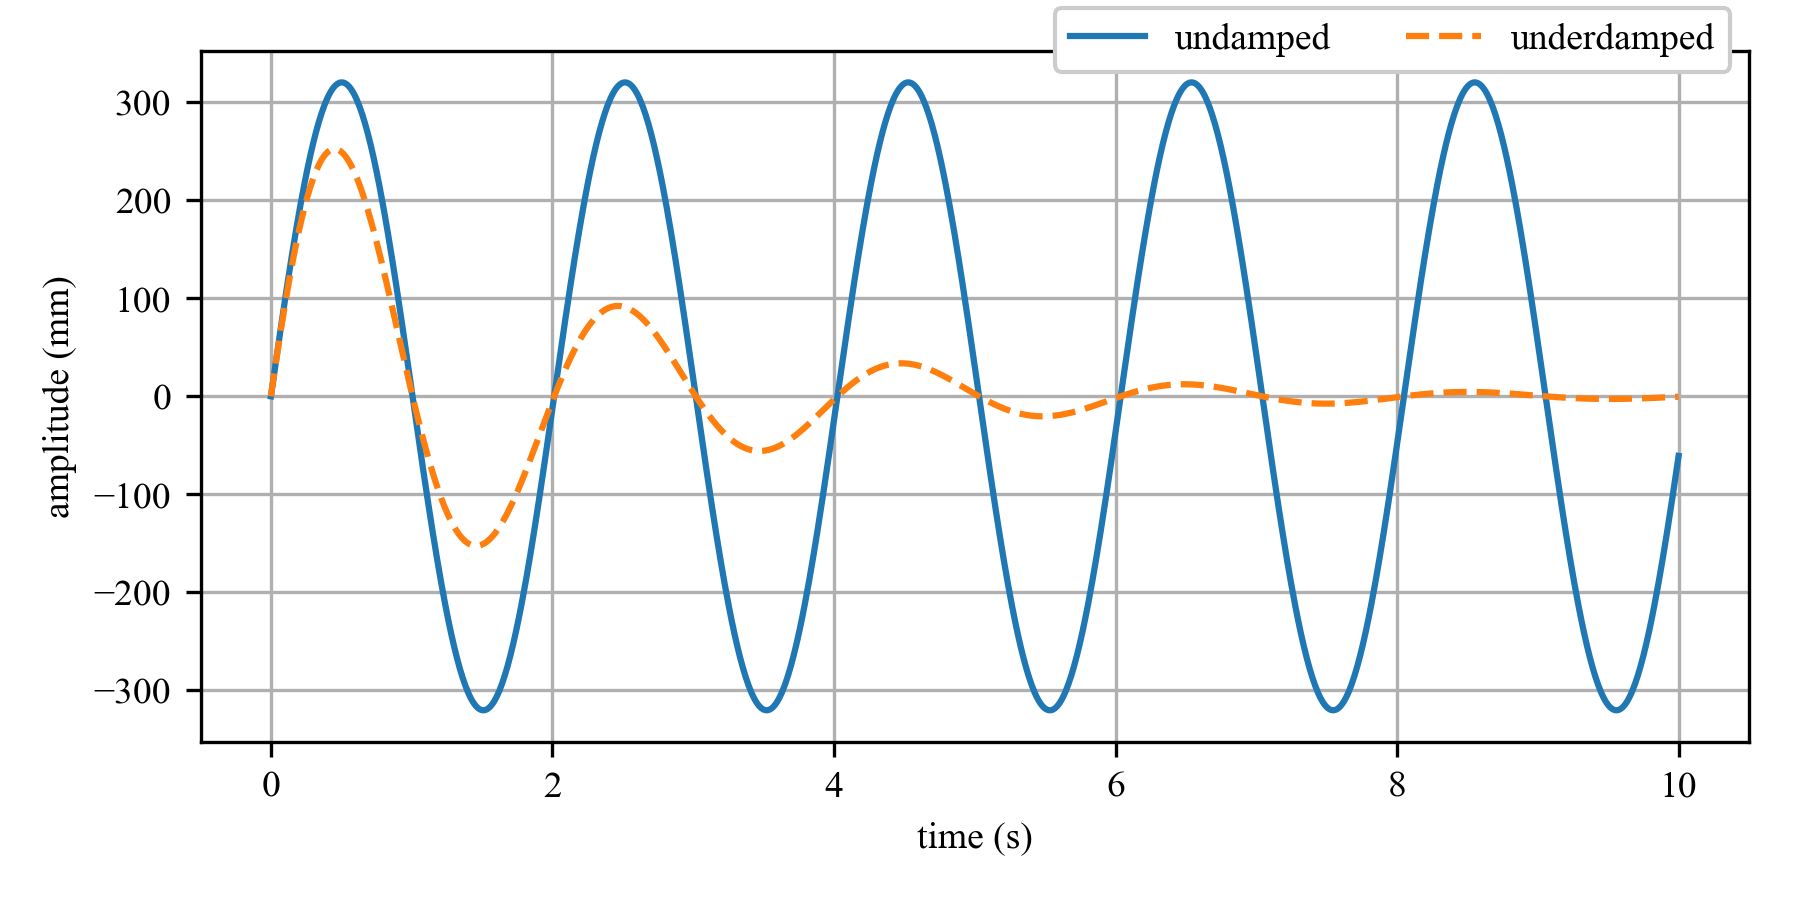
\includegraphics[width=0.75\textwidth]{../Figures/response_impulse.png}
\end{figure}



\subsubsection{Unit step function}
Now consider a unit step function $\Phi$: 

\begin{figure}[H]
	\centering
	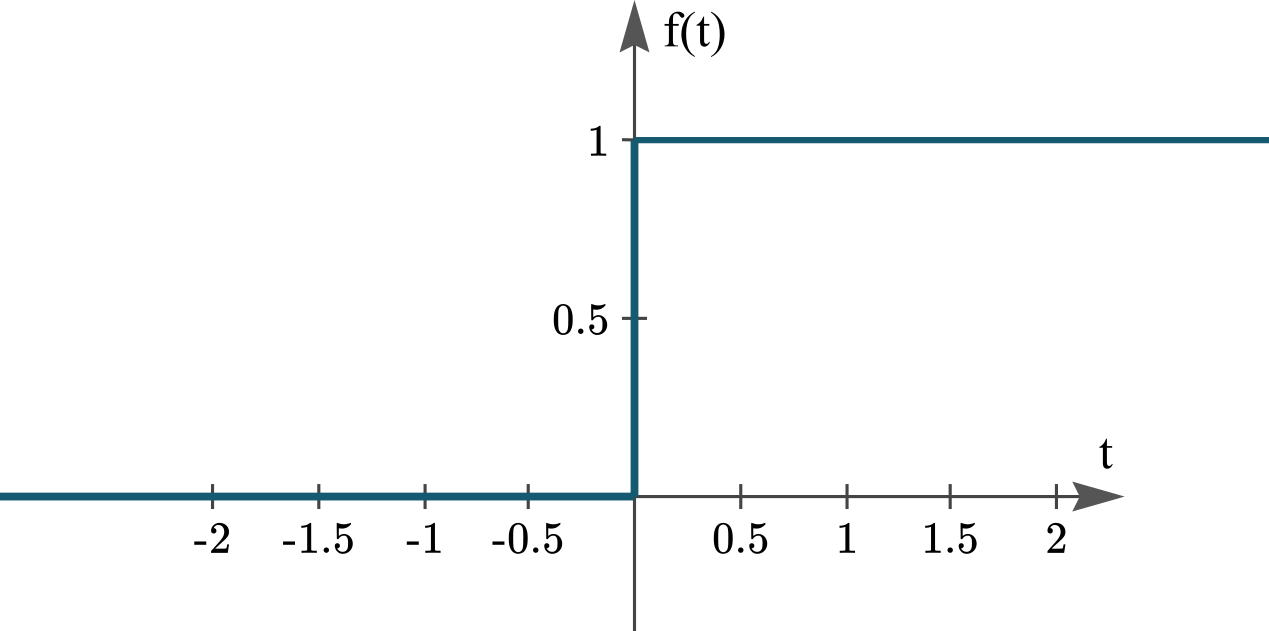
\includegraphics[width=0.5\textwidth]{../Figures/unit_step_function.png}
\end{figure}

A step function is a common loading situation and can represent the dropping of a load into a truck, a car going over a curve, or a motor starting up. 


The Laplace transform of the function, for a unit step function $\Phi$, is: 
\begin{equation*}
\Laplace{\Phi(t)} = \int_{0}^{\infty} e^{-st}dt = -\frac{e^{-\infty}}{s} +\frac{e^{-0}}{s} =\frac{1}{s}
\end{equation*}
This also lines up with Laplace Transform \# 3 from the attached table. This would be expected as $\Phi$ is used to represent the unit step function (i.e. a step function with a displacement of 1). As we consider linear systems in this class, we can scale the magnitude of the response by the magnitude of the impulse after the transform is performed. 

\subsubsection{Undamped spring-mass system}

For a spring-mass system subjected to a unit step, \textbf{assuming both initial conditions are zero}, the solution can be obtained using the transform method. First, the EOM is 
\begin{equation}
m\ddot{x}(t) + kx(t) = \Phi(t)
\end{equation}
Taking the Laplace transform of both sides and assuming zero initial conditions yields:
\begin{equation}
	ms^2X(s)+kX(s) =\frac{1}{s}
\end{equation}
Next, this equation is solved for $X(s)$ as:
\begin{equation}
	X(s) = \frac{1}{s(ms^2+k)}
\end{equation}
This can be rearranged as:
\begin{equation}
	X(s) = \frac{1}{m} \cdot \frac{1}{s(s^2+\omega_n^2)}
\end{equation}
where $\frac{1}{m}$ will pass through the Laplace function. Therefore, taking the inverse Laplace transform yields:
\begin{equation}
	x(t) = \frac{1}{m} \cdot \frac{1}{\omega_n^2}\big(1-\text{cos}(\omega_n t)\big) = \frac{1}{k}\big(1-\text{cos}(\omega_n t)\big)
\end{equation}
 
\subsubsection{Under damped spring-mass system}

For a spring-mass-damper system subjected to a unit step, assuming both initial conditions are zero, the solution can be obtained using the transform method. First, the EOM is:
\begin{equation}
m\ddot{x}(t) + c\dot{x} + kx(t) = \Phi(t)
\end{equation}
Converting to the standard form results in:
\begin{equation}
\ddot{x}(t) + 2  \zeta \omega_n\dot{x} + \omega_n^2x(t) = \frac{1}{m} \cdot \Phi(t)
\end{equation}
taking the Laplace transform of both sides and assuming zero initial conditions yields:
\begin{equation}
	s^2X(s) + 2  \zeta \omega_n s X(s) + \omega_n^2 X(s)  =\frac{1}{m} \cdot \frac{1}{s}
\end{equation}
Next, this equation is solved for $X(s)$ as:
\begin{equation}
	X(s) = \frac{1}{s^2 + 2  \zeta \omega_n s + \omega_n^2} \cdot \frac{1}{m} \cdot \frac{1}{s}
\end{equation}
multiplying the right-hand-side of this equation by  $\frac{\omega_n^2}{\omega_n^2}$ results in:
\begin{equation}
	X(s) = \frac{1}{m \omega_n^2} \cdot \frac{\omega_n^2}{s(s^2+2\zeta\omega_n s+\omega_n^2)}
\end{equation}
Again, the $\frac{1}{m\omega_n^2}$ will pass through the Laplace function. Therefore, taking the inverse Laplace transform yields:
\begin{equation}
	x(t) = \frac{1}{m \omega_n^2} \cdot \Big(1 - \frac{\omega_n}{\omega_d}e^{-\zeta \omega_n t}\text{sin}(\omega_dt + \phi)\Big)\text{, where } \phi = \text{cos}^{-1}(\zeta)\text{, where } \zeta<1
\end{equation}
After obtaining equations for the undamped and under damped cases, the responses for the unit step, solved with the transform method, can be plotted as:
\begin{figure}[H]
	\centering
	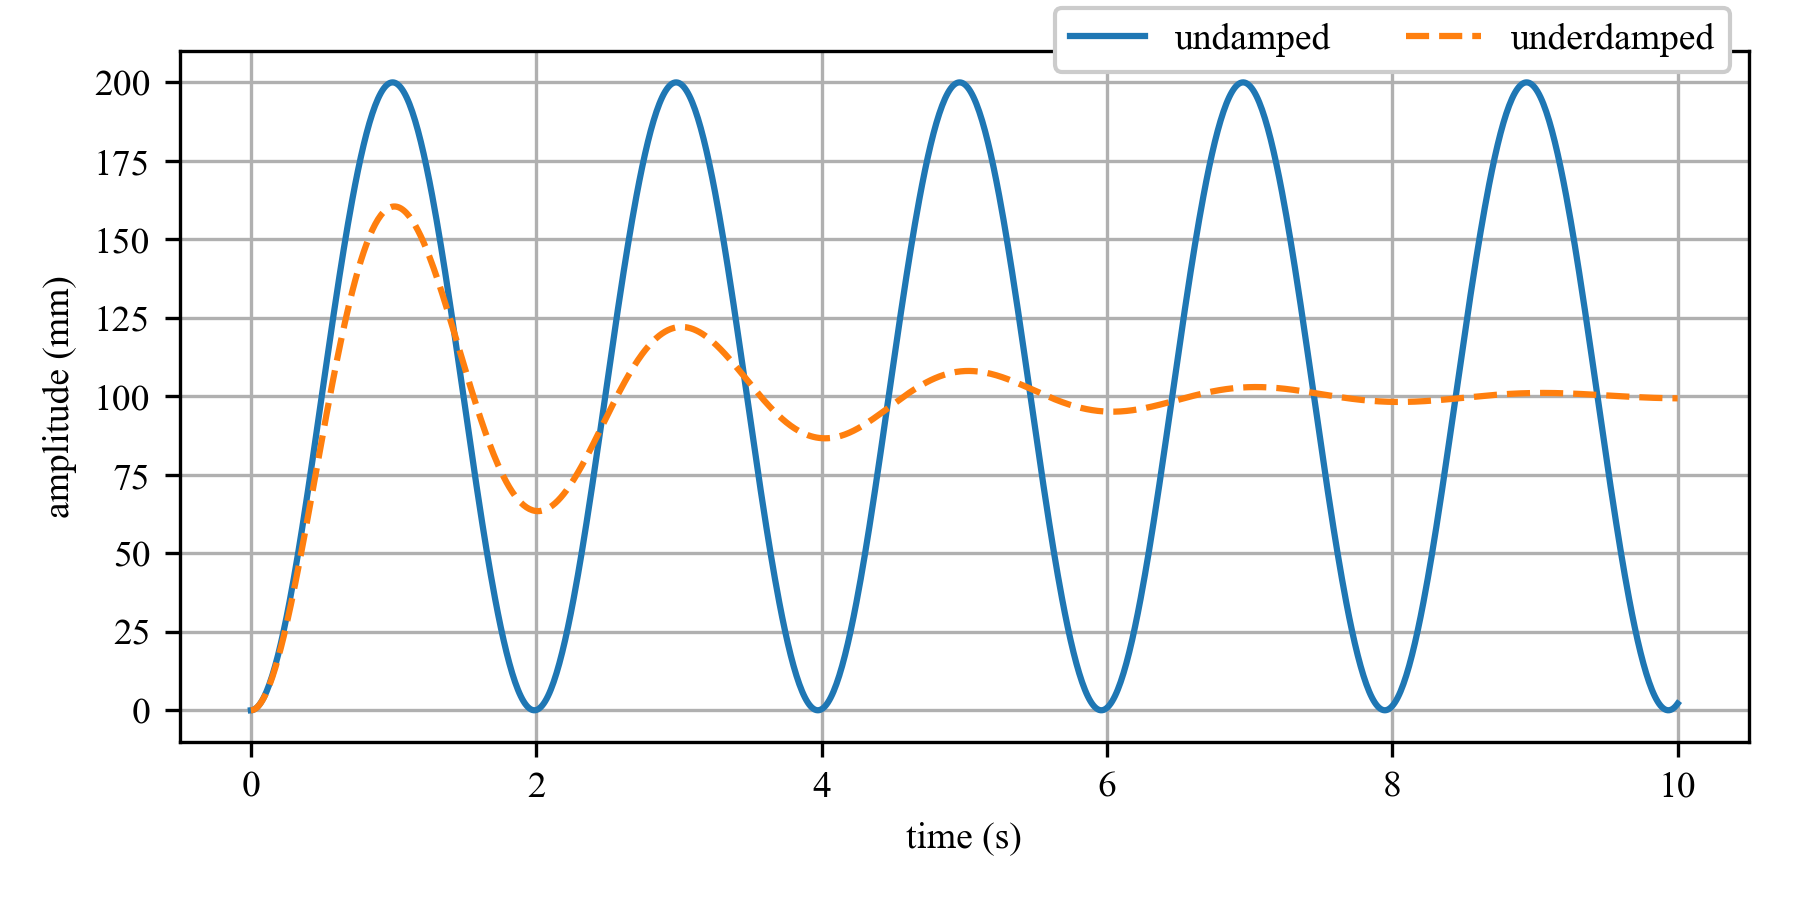
\includegraphics[width=0.75\textwidth]{../Figures/unit_step.png}
\end{figure}
Note that the system will settle out around $F_0/k$ where $F_0  \Phi$ is a scaling factor for the step loading.

\begin{example}
A load of roosters $m_r$ is dropped on the floor of a truck bed. Assuming the roosters do not move and that the truck bed is modeled as a spring-mass-damper system (of values $k$, $m$, and $c$, respectively).The load is modeled as a force $F(t) = m_r g$ applied to the spring-mass-damper system, as illustrated
in the following figure. This allows a crude analysis of the response of the truck's suspension. First assume that the trucks damper is broken, how does the maximum dynamic displacement compare to the static displacement. What would happen to the maximum displacement if the damper was repaired on the truck? %Next, using a damping value of $\zeta=0.5$ and $\omega_n=\pi$ what is the maximum displacement. How does this compare to the displacement for the case without the damper?  

\begin{figure}[H]
	\centering
	\includegraphics[width=0.8\textwidth]{../Figures/dump_truck_example.png}
	\caption{Dump truck being loaded with roosters showing (a) roosters going into the truck bed; and (b) the single-degree-of-freedom vibration model.}
\end{figure}

\textbf{Solution }

First, setting the load applied to the truck as 1 unit, it can be seen that this is a unit step loading condition and a broken damper represents an undamped case. To obtain a rough idea about the nature of static and dynamic displacement, the undamped displacement is

\begin{equation}
	x(t) = \frac{1}{k}\big(1-\text{cos}(\omega_n t)\big) = \frac{m_dg}{k}\big(1-\text{cos}(\omega_n t)\big)
\end{equation}
 
This equation has a maximum amplitude when the cos$(\omega_dt)=-1$, resulting in:
\begin{equation}
	x(t) = \frac{m_dg}{k}\big(1-(-1)\big)
\end{equation}
This can be rearranged for the maximum displacement value $x_\text{max} $ as:
\begin{equation}
	x_\text{max} = 2\frac{m_dg}{k}
\end{equation} 
This is twice the static displacement (i.e., twice the distance the truck would be deflected if the dirt were placed gently and slowly onto it). Thus, if the truck were designed with springs based only on the static load, with no margins of safety, the springs in the truck
would potentially break, or permanently deform, when subjected to the same mass applied dynamically (e.g., dropped) into the truck. Hence, it is important to consider the vibration (dynamic) response in designing structures that could experience dynamic loading.

%\textbf{Example 1 - under damped}
%For the case where the truck has a damper with a value of $\zeta=0.5$, the displacement $(x)$ can be modeled as:
%\begin{equation}
%	x(t) = \frac{m_dg}{m \omega_n^2} \cdot \Big(1 - \frac{\omega_n}{\omega_d}e^{-\zeta \omega_n t}\text{sin}(\omega_dt + \phi)\Big)\text{, where } \phi = \text{cos}^{-1}(\zeta)
%\end{equation}

\end{example}
\begin{example}


In testing, an hammer is used to excite a 1-DOF system with an impact (i.e. impulse), however, the hammer ascendantly impacts the system twice. The first impact has a force of 0.2 N, while the second has a force of 0.1 N and happens 0.1 seconds after the first impact. Plot the response for the double impact. The system has the parameters $m$ = 1 kg, $c$ = 0.5 kg/s, k = 4 N/m. 

\textbf{Solution }

First, we can define the forcing function as:

\begin{equation}
	F(t) = 0.2 \delta (t) + 0.1 \delta(t-\tau)
\end{equation}
where $\tau$ is the offset between the first and second impacts. Next, considering that the unit impulse has a magnitude of 1 we can obtain solutions for the first impact by first writing it's EOM:

\begin{equation}
m\ddot{x} +c\dot{x} +kx =0.2 \delta(t)
\end{equation}
Taking the Laplace transform of both sides of the equation yields 
\begin{equation}
m\big(s^2X(s)-sx(0) - \dot{x}(0)\big) + c\big(sX(s)-x(0)\big) +kX(s) = 0.2
\end{equation}
However, assuming zero initial conditions, the equation simplifies to. 
\begin{equation}
(ms^2 + cs +k)X(s) = 0.2
\end{equation}
Solving this equation for $X(s)$:
\begin{equation}
X(s) = \frac{0.2}{m} \cdot \frac{1}{s^2 + 2 \zeta \omega_n s + \omega_n^2}
\end{equation}
Again, consulting \#10 in the table for Laplace transforms results in:
\begin{equation}
x_1(t) = \frac{0.2}{m \omega_d} e^{-\zeta \omega_n t} \text{sin}(\omega_dt)
\end{equation}
where this is the general solution for a damped system subjected to an impulse loading function. The second impact can now be solved for using the same method. However, now the time $(t)$ must be offset by $(\tau)$ to allow the impact to still be located at $t=0$ in terms of the second impact. This results in:
\begin{equation}
	x_1(t) = \frac{0.2}{m \omega_d} e^{-\zeta \omega_n t} \text{sin}(\omega_dt)
\end{equation}
\begin{equation}
	x_2(t) = \frac{0.1}{m \omega_d} e^{-\zeta \omega_n (t-\tau)} \text{sin}\big(\omega_d(t-\tau)\big)
\end{equation}
Next, using the knowledge that the systems are linear and that the Laplace transform of a linear combination of two transforms is the same as the linear transformation of these functions we can build the piecewise function:

\[
  x(t) = x_1(t) + x_2(t) =
  \begin{cases}
\frac{0.2}{m \omega_d} e^{-\zeta \omega_n t} \text{sin}(\omega_dt) & \text{if } t < \tau \\
\frac{0.2}{m \omega_d} e^{-\zeta \omega_n t} \text{sin}(\omega_dt)  + \frac{0.1}{m \omega_d} e^{-\zeta \omega_n (t-\tau)} \text{sin}(\omega_d(t-\tau) & \text{if } \tau \leq t 
  \end{cases}
\]


For the mass, damping, and stiffness values given above this can be plotted as:
\begin{figure}[H]
	\centering
	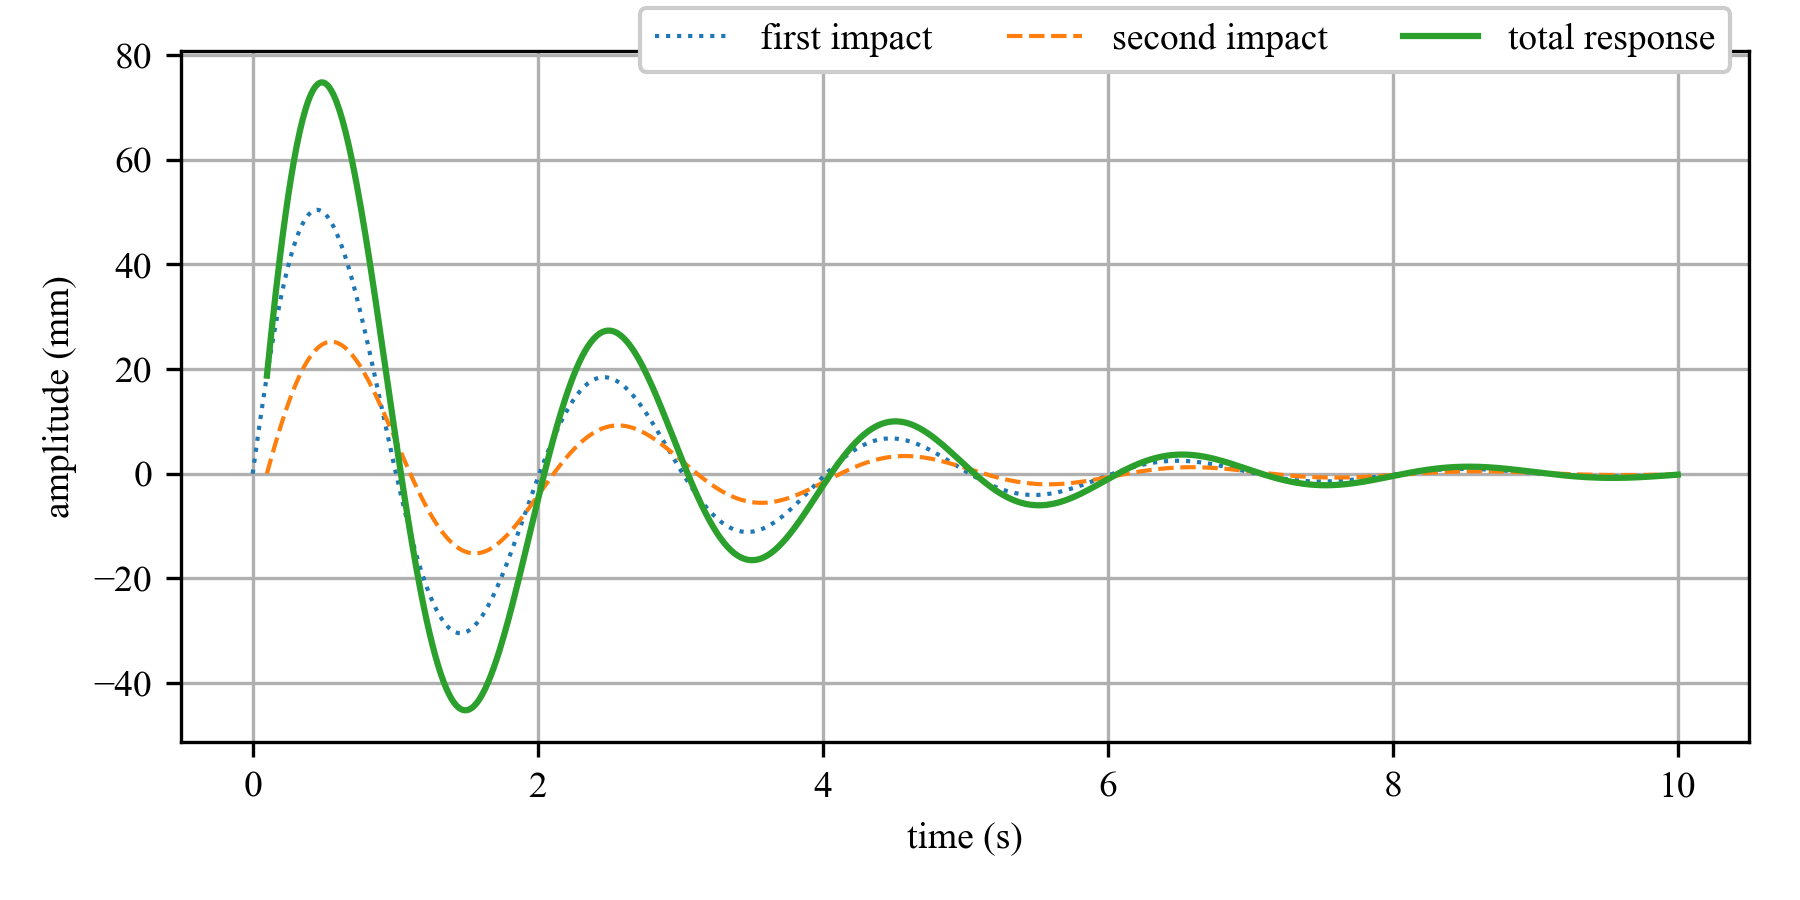
\includegraphics[width=0.75\textwidth]{../Figures/response_double_impact.png}
\end{figure}

\end{example}


\subsection{Transform function for response to random inputs}
	
\subsubsection{Defining the transfer function $\mathbf{H(s)}$}

Again, consider the following system
\begin{figure}[H]
	\centering
	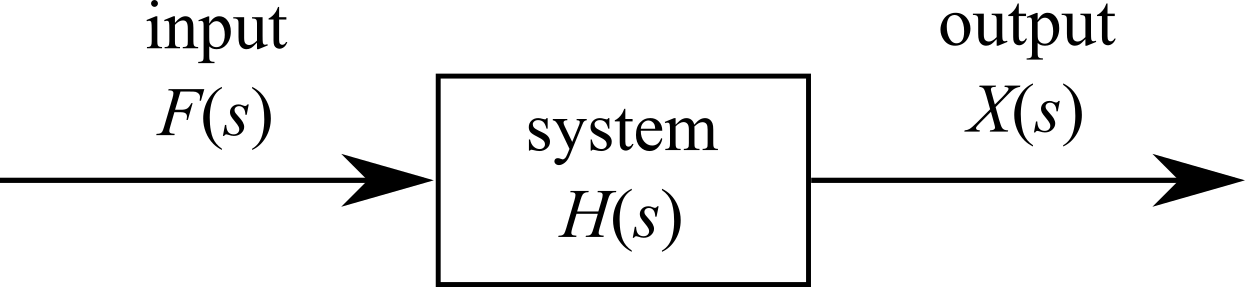
\includegraphics[width=0.5\textwidth]{../Figures/system_input_output.png}
\end{figure}
For this system representation, F(s) is the Laplace of the transform of the driving force and H(s) is the Laplace transform of the response of the system h(t). 

We need to define transfer function $H(s)$ for a generic system. To do this let us show the reasoning behind the transfer function. \textbf{Here we will show that the output of any system ($x(t)$) can be related to the input of the system ($f(t)$) through a series of polynomial coefficients ($a$ and $b$).} Consider the general $n^{th}$-order linear, time-invariant differential equation that governs the behavior of the dynamic system.

\begin{equation}
a_n\frac{d^nx(t)}{dt^n} + a_{n-1}\frac{d^{n-1}x(t)}{dt^{n-1}} + ... + a_0x(t) = b_m\frac{d^mf(t)}{dt^m} + b_{m-1}\frac{d^{m-1}f(t)}{dt^{m-1}} + ... + b_0f(t)
\end{equation} 
where $x(t)$ is the output and $f(t)$ is the input. Note that this is similar to the formulation we have had before for the EOM. Taking the Laplace transformation of both side of the above equation yields

\begin{eqnarray}
&a_ns^nX(s) + a_{n-1}s^{n-1}X(s) + ... + a_0X(s) + \text{initial condition involving } x(t) =   \\
&b_ms^mF(s) + b_{m-1}s^{m-1}F(s) + ... + b_0F(s) + \text{initial condition involving } f(t)  \nonumber
\end{eqnarray}
It can be seen that this equation is a purely algebraic expression. If we assume the initial conditions to be zero, the equation reduces to the following:
\begin{eqnarray}
(a_ns^n + a_{n-1}s^{n-1} + ... + a_0)X(s) =  (b_ms^m + b_{m-1}s^{m-1} + ... + b_0)F(s) 
\end{eqnarray}
we can rearrange the equation as 
\begin{equation}
H(s) = \frac{X(s)}{F(s)} = \frac{b_ms^m + b_{m-1}s^{m-1} + ... + b_0}{a_ns^n + a_{n-1}s^{n-1} + ... + a_0}
\end{equation}
where H(s) is the \textbf{transfer function} that is defined as:

\textit{The ratio of the Laplace transforms of the output or response function to the laplace transform of the input or forcing function assuming zero initial conditions.}

This can be rearranged to show that the output of the system $X(s)$ can be obtained if we know the input $F(s)$ and the transfer function $H(s)$:
\begin{equation}
X(s) = H(s)F(s)
\end{equation}	


\subsubsection{Transfer Function method (Steady-State solution)}

Considering the forced system:
\begin{figure}[H]
	\centering
	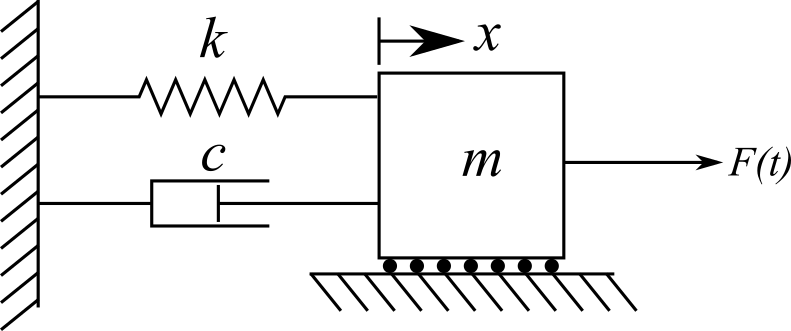
\includegraphics[width=0.4\textwidth]{../Figures/forced_spring_mass_damper_system.png}
\end{figure}
that can be expressed as the equation of motion
\begin{equation}
	m\ddot{x} + c\dot{x} +kx = F_0 \cos(\omega t)
\end{equation}
Here $F_0 \cos(\omega t)$, is used at the input but any input will develope the same transfer function as the transfer function is bounded to the system and not the input. From the \#6 in the table for Laplace Transforms, we know that
\begin{equation}
	\Laplace{\cos(\omega t)} = \frac{s}{s^2+\omega^2}
\end{equation}
Therefore, 
\begin{equation}
F(s) = \frac{F_0s}{s^2+\omega^2}
\end{equation}
Ignoring the initial conditions, and therefore considering only the partial solution, and taking the Laplace transform of the EOM equation yields:
\begin{equation}
(ms^2 + cs +k)X(s) = \frac{F_0s}{s^2+\omega^2} 
\end{equation}
where $s$ is the complex transform variable and $X(s)$ denotes the Laplace transform of the unknown function x(t). Solving algebraically for the $X(s)$ yields: 
\begin{equation}
X(s) = \frac{F_0s}{(ms^2 + cs +k)(s^2+\omega^2)}
\end{equation}
Now that we have $F(s)$ and $X(s)$ we can obtain $H(s)$ as  
\begin{equation}
H(s) = \frac{X(s)}{F(s)} = \frac{F_0s}{(ms^2 + cs +k)(s^2+\omega^2)} \cdot \frac{s^2+\omega^2}{F_0s} = \frac{1}{ms^2+cs+k}
\end{equation}
or 
\begin{equation}
H(s) = \frac{1}{ms^2+cs+k}
\end{equation}
This ratio is termed the \textbf{transfer function of a system} and is an important tool in vibration analysis.

Recall that $s$ is a complex number, if the value of $s$ is restricted to lie along the imaginary axis in the complex plane (i.e., if $s = j\omega$), the transfer function becomes:
\begin{equation}
H(j\omega) = \frac{1}{m(j\omega)^2+cj\omega+k} = \frac{1}{-m\omega^2+cj\omega+k} 
\end{equation}
rearranging into a standard form yields:
\begin{eqnarray}
H(j\omega) = \frac{1}{k-m\omega^2+c\omega j}
\end{eqnarray}
recall that $j^2=-1$. This is the \textbf{frequency response function of the system}. Therefore, it can bee seen that the frequency response function of the system is the transfer function of the system evaluated along the imaginary axis $s=j\omega$. However, this expression contains imaginary values (that help to account for the phase in the system) and therefore can be challenging to work with. If we ignore the phase component and only consider the amplitude $|H(j\omega)|$ of the response (the real portion of the equation) we get:
\begin{eqnarray}
H(\omega) = |H(j\omega)| = \frac{1}{\sqrt{(k-m\omega^2)^2+c^2\omega^2}}
\end{eqnarray}
where $|H(j\omega)|$ represents only the amplitude of the frequency response function. A more detailed derivation can be found in [Mechanical Vibrations - Rao, 6th edition]



To recap, for a single DOF damped spring-mass system the \textbf{transfer function} is:
\begin{equation}
H(s) = \frac{1}{ms^2+cs+k}
\end{equation}
And the \textbf{frequency response function} is:
\begin{eqnarray}
H(j\omega) = \frac{1}{k-m\omega^2+c\omega j}
\end{eqnarray}
While the amplitude of the frequency response is:
\begin{eqnarray}
H(\omega) = |H(j\omega)| = \frac{1}{\sqrt{(k-m\omega^2)^2+c^2\omega^2}}
\end{eqnarray}




\subsubsection{Response to Random Inputs}
The transfer and frequency response functions can be very useful for demeriting the response to random inputs. Up to this point we have solved for deterministic input. 

\begin{itemize}
\item \textbf{Deterministic}-For a known time $t$, the value of the input force $F(t)$ is precisely known. 
\item \textbf{Random} For a known time $t$, the value of the input force $F(t)$ is known only statistically. 
\end{itemize}

To expand, a random signal is a signal with no obvious pattern. For these types of it is not possible to focus on the details of the input signal, as is done with a deterministic signal, rather the signal is classified and manipulated in terms of its statistical properties. 

Randomness in vibration analysis can be thought of as the result of a series of results obtained from testing a system repeatability for various inputs under varying conditions. In these cases, one record or time history is not enough to describe the system. Rather, an ensemble of various tests are used to describe how the system will respond to the various inputs. 

First, let us consider two inputs, a deterministic input (typical sin wave), and a random input (white noise). These inputs are shown below. 

\begin{figure}[H]
	\centering
	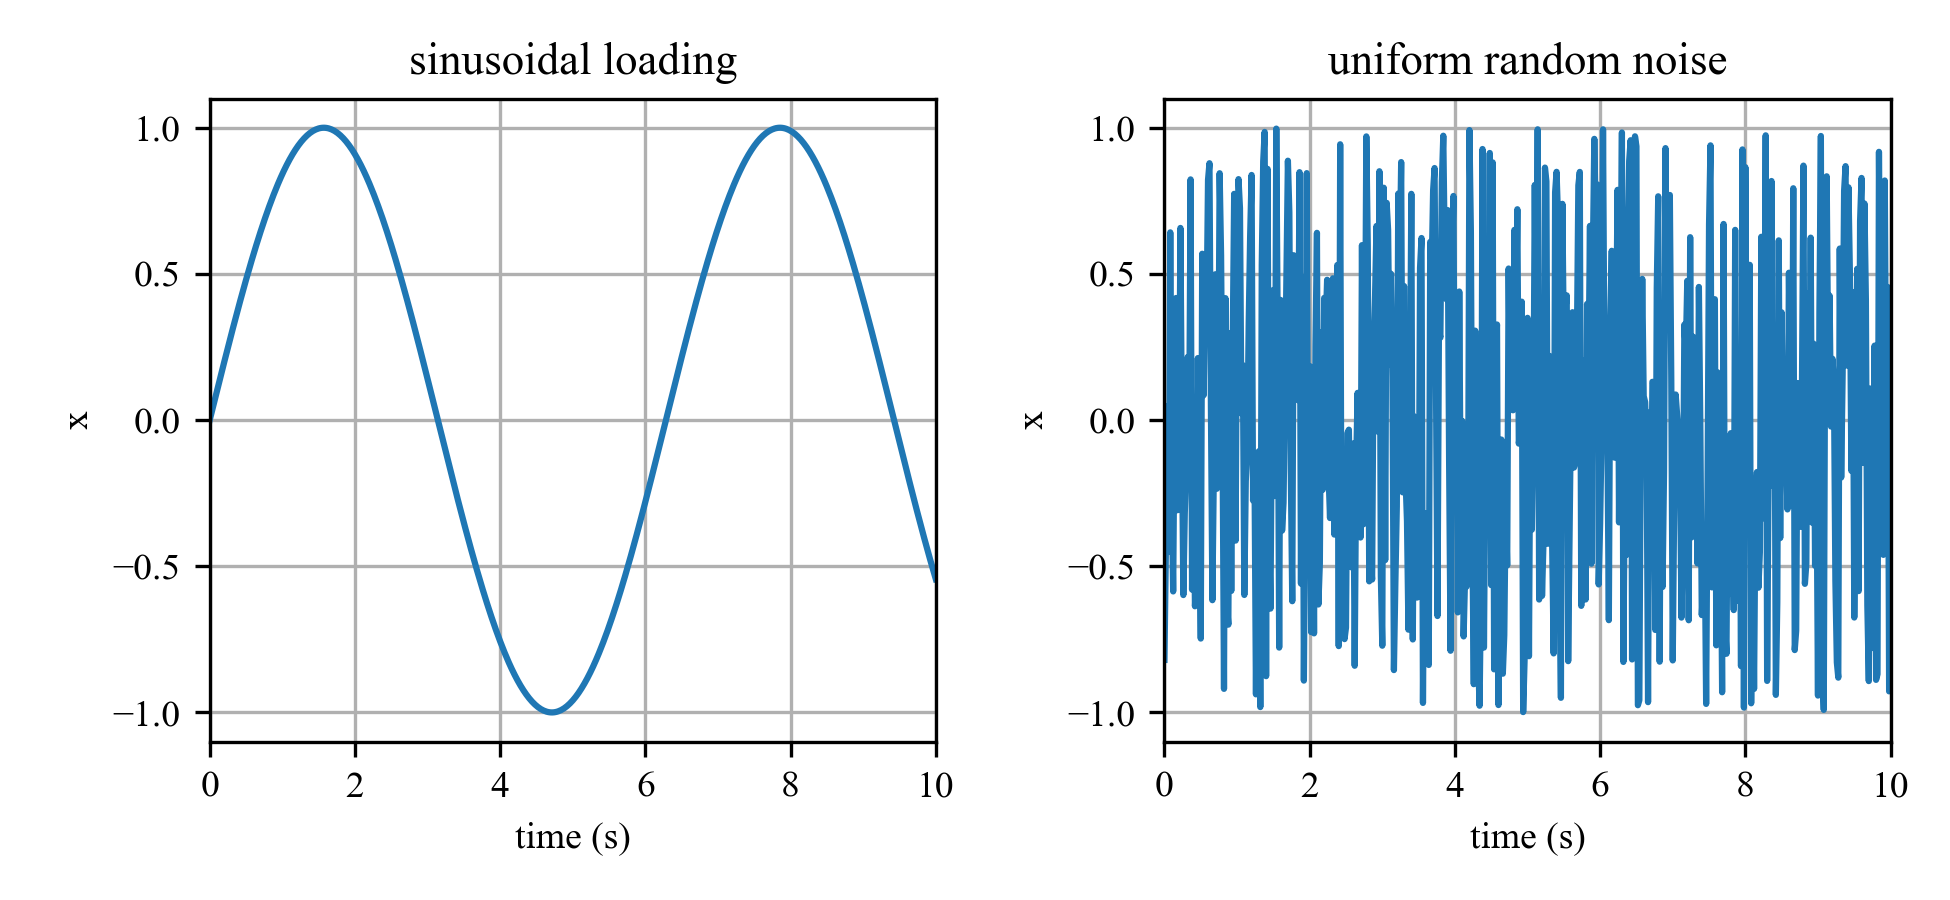
\includegraphics[width=1\textwidth]{../Figures/Response_to_random_input_inputs.png}
\end{figure}

One of the fist factors to consider is the \textbf{mean of the random signal} $x(t)$, defined as:

\begin{equation}
E[x] = \bar{x} = \lim\limits_{T \rightarrow \infty} \frac{1}{T} \int_{0}^{T}x(t)dt
\end{equation}

where $T$ is the length in time of the data collected. However, for random signals we often want to consider signals with an average mean of zero (i.e. $\bar{x}(t)=0$). Therefore, for signals not centered around zero we can obtain a zero centered signal if the signal is stationary and we subtract the mean value from $\bar{x}$ from the signal $x(t)$. This can be written as:

\begin{equation}
x'(t) = x(t) - \bar{x}
\end{equation} 

where the $x'(t)$ is now centered around zero. As mentioned before, it is important to consider whether or not the input signals are stationary. A signal is \textbf{stationary} if its statistical properties (usually expressed by its mean) do not change with time. Here, it can be seen that for our inputs considered the signals are stationary if a long enough time period is considered. 

Another important variable is \textbf{variance} (or mean-square value) of the random variable $x(t)$ defined as:
\begin{equation}
E[x^2] = \bar{x^2} = \lim\limits_{T \rightarrow \infty} \frac{1}{T} \int_{0}^{T}x^2(t)dt
\end{equation}

and provides a measure of the magnitude of the fluctuations in the signal $x(t)$. This gives an easy way to calculate the root-mean-square (RMS) of the signal as:
\begin{equation}
x_\text{rms} = \sqrt{\bar{x^2}} 
\end{equation}

Now, considering the actual signal, a important measure of interests is how fast the value of the variables change. This is important to understand as it address how long it takes to measure enough samples of the variable before a meaningful statistical value can be calculated. One way to quantify how fast the values of signal change is the \textbf{autocorrelation function}: 
\begin{equation}
R_{xx}(\tau) = \lim\limits_{T \rightarrow \infty} \frac{1}{T} \int_{0}^{T}x(t)x(t+\tau)dt
\end{equation}
The subscript $xx$ denotes that this is a measure of the response for the variable xx, $\tau$ is the time difference between the values at which the signal $x(t)$ is sampled. The auto collation for the two inputs considered above are expressed below:
\begin{figure}[H]
	\centering
	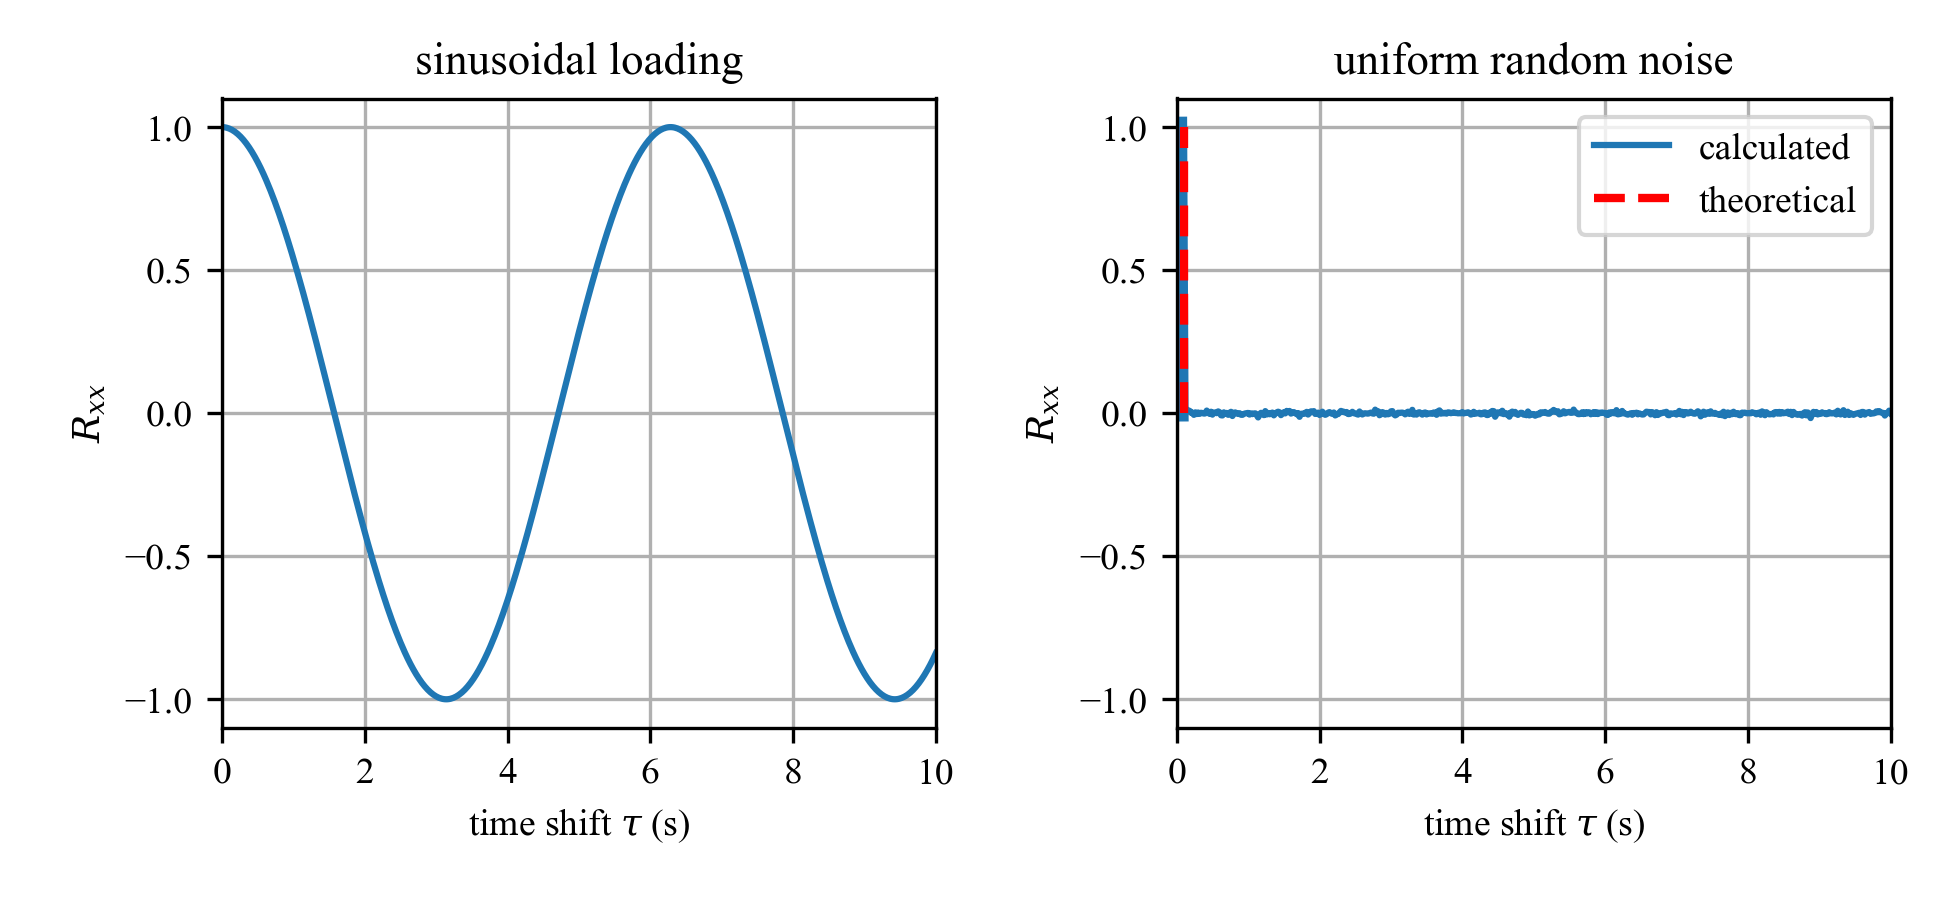
\includegraphics[width=1\textwidth]{../Figures/Response_to_random_input_autocorrelation.png}
\end{figure}
Note that the value of $\tau$ selected in the auto correlation function greatly affects its response for the sinusoidal input. This is because the values for the sinusoidal are high correlated. To expand, the value at any time $t$ is greatly effected by the values immediately before and after it. This is not the case for the random input where the signal is not correlated and therefore there is little difference in changing the value of $\tau$ on the response of the autocorrelation function.  

Next, if we take the Fourier transform of the autocorrelation function we obtain the power spectral density (PSD) defined as:
\begin{equation}
S_{xx}(\omega) =\frac{1}{2 \pi} \int_{-\infty}^{\infty} R_{xx}(\tau) e^{-j \omega \tau}d \tau
\end{equation}
where the integral of $R_{xx}(\tau)$ changes the real number $\tau$ into the frequency-domain value $\omega$. The frequency spectrum (hence the $S$ in $S_{xx}(\omega)$) for the two input cases considered are plotted below.
\begin{figure}[H]
	\centering
	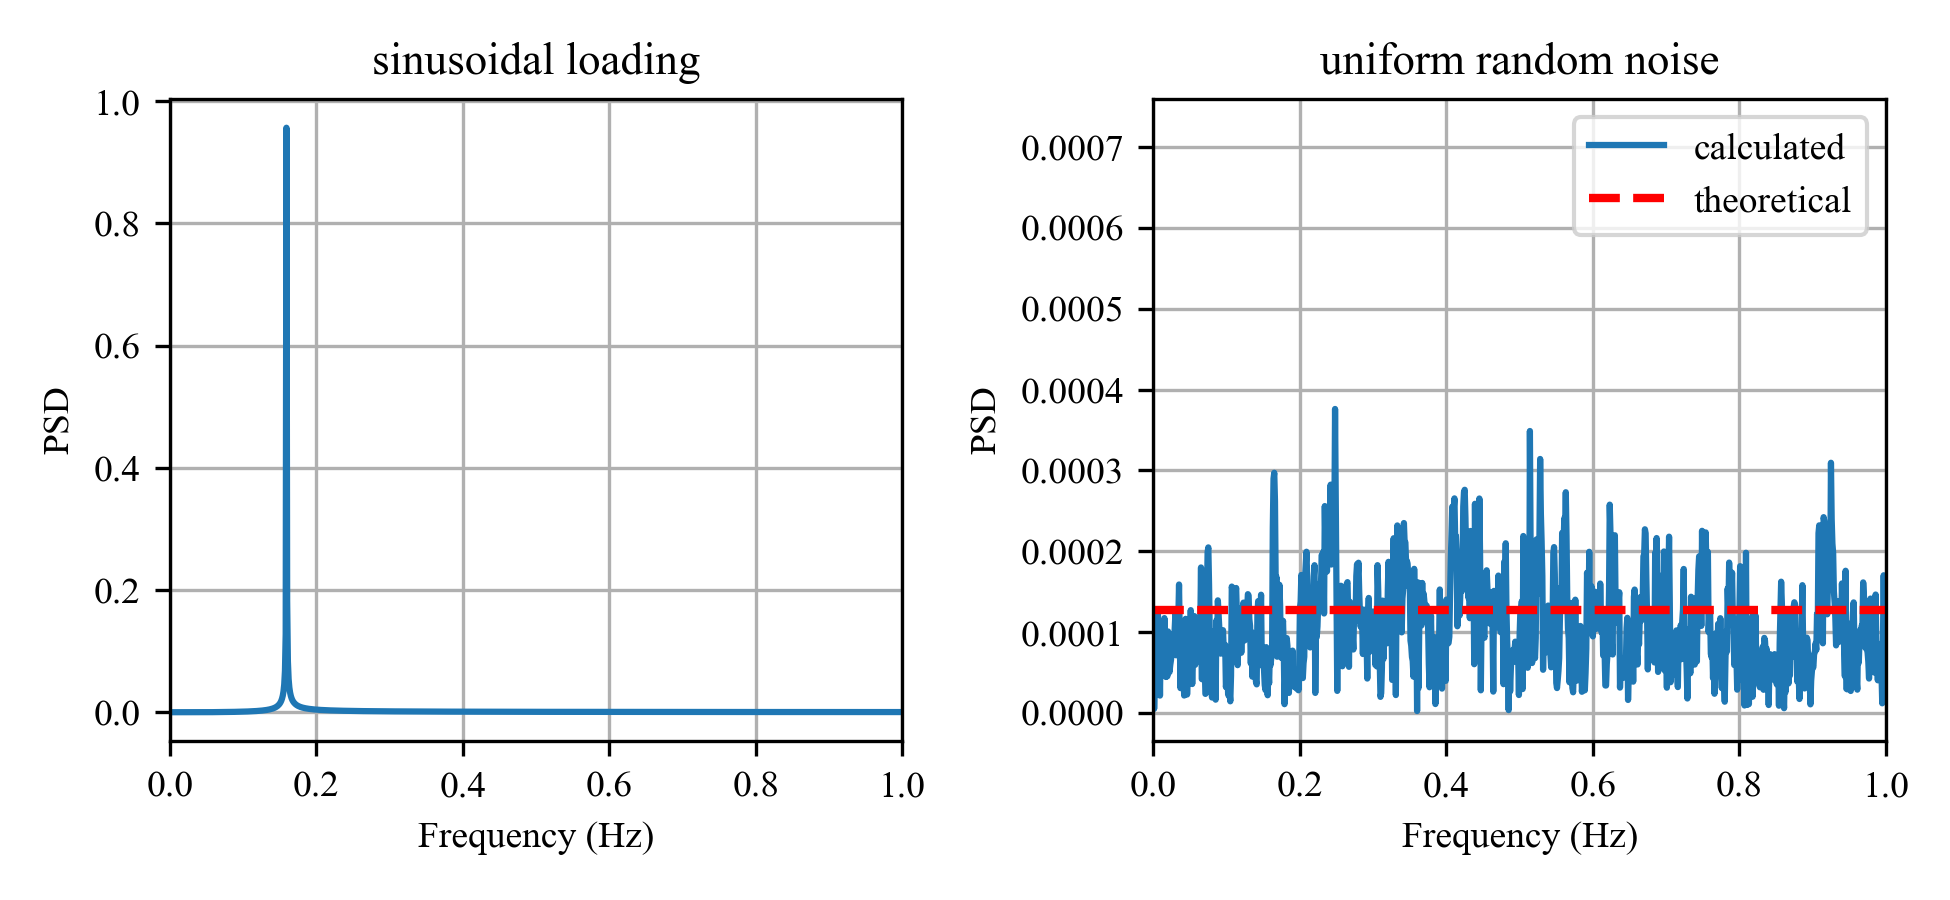
\includegraphics[width=1\textwidth]{../Figures/Response_to_random_input_PSD.png}
\end{figure}
where the flat frequency response for the random input denotes that the random input is white noise input. A true white noise input would be perfectly flat, and is really just a theoretical concept. 

Recall that $S_{xx}$ is the spectrum of the response of the system. For the one-DOF system considered here, we can express an arbitrary input as a series of impulse inputs. 
\begin{figure}[H]
	\centering
	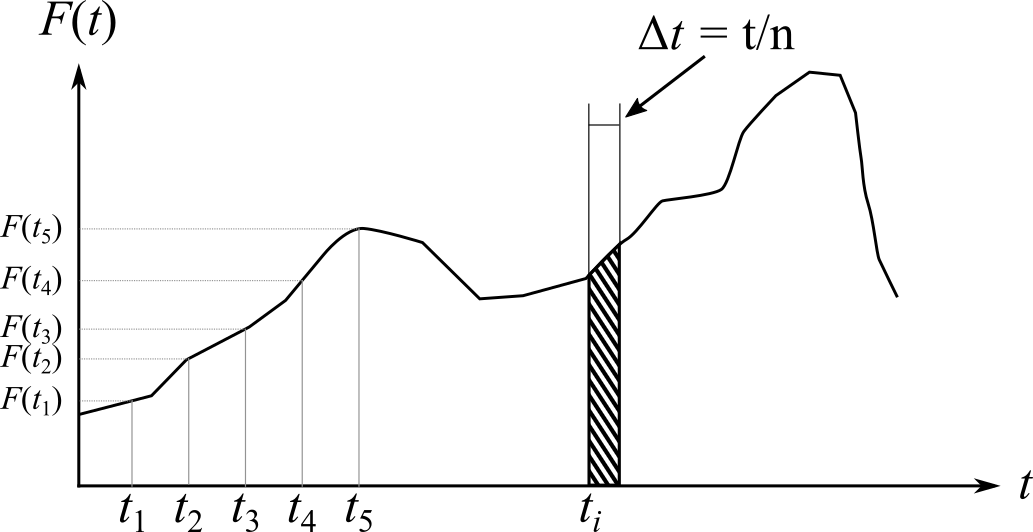
\includegraphics[width=0.7\textwidth]{../Figures/Arbitary_excitation_forces.png}
\end{figure}
This knowledge, along with the frequency response function can be used to relate the spectrum of the input $S_{ff}(\omega)$ to the output through the transfer function as:
\begin{equation}
S_{xx}(\omega) =  |H(j\omega)|^2\Bigg[\frac{1}{2 \pi } \int_{-\infty}^{\infty} R_{ff}(\tau) e^{-j \omega \tau}d  \tau  \Bigg] 
\end{equation}
This can also be expressed in symbolic form as
\begin{equation}
S_{xx}(\omega) =  |H(j\omega)|^2 S_{ff}(\omega)
\end{equation}
where $R_{ff}$ denotes the autocorrelation function of $F(t)$ and $S_{ff}$ denotes the PSD of the forcing function $F(t)$. The notation $|H(j\omega)|^2$ is the square of the magnitude of the complex frequency response function. A more detailed derivation can be found in [Engineering Vibrations, Inman (2001)],[Random Vibrations, Spectral \& Wavelet Analysis, Newland (1993)], but here it is more important to study the results rather than the derivations. 

Another useful quantity to consider is the expected value of the output for a given input. The expected value $E[x]$, or $\bar{x}$, is expressed as:
\begin{equation}
E[x] =  \lim\limits_{T\rightarrow\infty} \int_{0}^{T} \frac{x(t)}{T}dt
\end{equation}
Additionally, the mean-square value can be directly related to the PSD function as 
\begin{equation}
E[x^2] = \bar{x^2} =   \int_{-\infty}^{\infty} |H(j\omega)|^2 S_{ff}(\omega) d\omega
\end{equation}
Moreover, for a constant input $S_{ff}(\omega) = S_0$ in therms of the frequency domain, the mean-square value can be expressed as:
\begin{equation}
E[x^2] = \bar{x^2} =   S_{0} \int_{-\infty}^{\infty} |H(j\omega)|^2 d\omega
\end{equation}

After inspecting the above equation, it becomes clear that to obtain the square of the expected value, a solution for  $\int_{-\infty}^{\infty} |H(j\omega)|^2$ must be obtained. For cases where $S_{ff}(\omega) = S_0$ and as such $S_{ff}(\omega)$ can be pulled out of the integral, these integrals have been solved [Random Vibrations, Spectral \& Wavelet Analysis, Newland (1993)]. For example, given $\int_{-\infty}^{\infty} |H(j\omega)|^2 d\omega$:

\begin{equation}
\int_{-\infty}^{\infty} \bigg|\frac{B_0}{A_0+j \omega A_1} \bigg|^2 d\omega = \frac{\pi B_0^2}{A_0 A_1}
\end{equation} 

and

\begin{equation}
\int_{-\infty}^{\infty} \bigg|\frac{B_0 + j \omega B_1}{A_0+j \omega A_1 - \omega^2 A_2} \bigg|^2 d\omega = \frac{\pi (A_0 B_1^2 + A_2 B_0^2)}{A_0 A_1 A_2}
\end{equation} 
When combined with the equation $E[x^2] = S_{0} \int_{-\infty}^{\infty} |H(j\omega)|^2 d\omega$, these integrals allow for the easy calculation of the expected values. 

\begin{example}

Considering the forced system:
\begin{figure}[H]
	\centering
	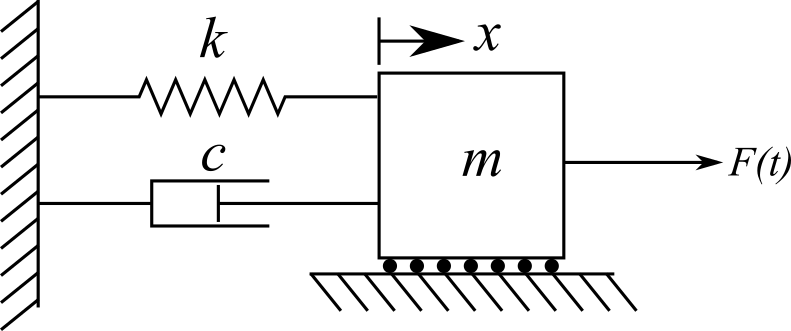
\includegraphics[width=0.4\textwidth]{../Figures/forced_spring_mass_damper_system.png}
\end{figure}
Set the forcing function to be $F_0 \sin(\omega t)$ and calculate the transfer function. 

\textbf{Solution}

that can be expressed as the equation of motion
\begin{equation}
	m\ddot{x} + c\dot{x} +kx = F_0 \sin(\omega t)
\end{equation}
From the \#6 in the table for Laplace Transforms, we know that
\begin{equation}
	\Laplace{\sin(\omega t)} = \frac{\omega}{s^2+\omega^2}
\end{equation}
Therefore, 
\begin{equation}
F(s) = \frac{F_0\omega}{s^2+\omega^2}
\end{equation}
Ignoring the initial conditions and taking the Laplace transform of the EOM equation yields:
\begin{equation}
(ms^2 + cs +k)X(s) = \frac{F_0 \omega}{s^2+\omega^2} 
\end{equation}
Solving algebraically for the $X(s)$ yields: 
\begin{equation}
X(s) = \frac{F_0\omega}{(ms^2 + cs +k)(s^2+\omega^2)}
\end{equation}
Now that we have $F(s)$ and $X(s)$ we can obtain $H(s)$ as  
\begin{equation}
H(s) = \frac{X(s)}{F(s)} = \frac{F_0 \omega }{(ms^2 + cs +k)(s^2+\omega^2)} \cdot \frac{s^2+\omega^2}{F_0 \omega} = \frac{1}{ms^2+cs+k}
\end{equation}
or 
\begin{equation}
H(s) = \frac{1}{ms^2+cs+k}
\end{equation}
This is identical to the solution obtained using $F_0 \cos(\omega t)$ as would be expected because the transfer function is related to the system and not to the input. 
\end{example}  


\begin{example}

Consider the following system

\begin{figure}[H]
	\centering
	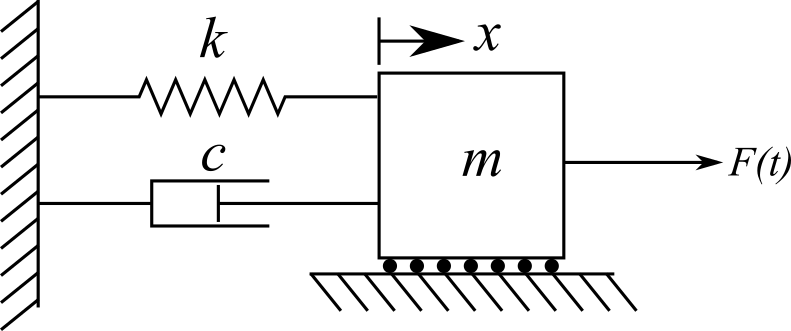
\includegraphics[width=0.4\textwidth]{../Figures/forced_spring_mass_damper_system.png}
\end{figure}

Calculate the PSD of the response $x(t)$ given that the PSD of the applied force $S_{ff}(\omega)$ is white noise. 

\textbf{Solution}

From the system we know that the EOM is 

\begin{equation}
m\ddot{x} +c\dot{x} + kx = F(t)
\end{equation} 
The frequency response function for this system is 
\begin{eqnarray}
	H(j\omega) = \frac{1}{k-m\omega^2+c\omega j}
\end{eqnarray}
while the amplitude of the response is:
\begin{eqnarray}
H(\omega) = |H(j\omega)| = \frac{1}{\sqrt{(k-m\omega^2)^2+c^2\omega^2}}
\end{eqnarray}
Applying the equation that relates $S_{ff}(\omega)$ to $S_{xx}(\omega)$ we get:
\begin{equation}
S_{xx}(\omega) =  |H(j\omega)|^2 S_{ff}(\omega) = \bigg|\frac{1}{k-m\omega^2+c\omega j} \bigg|^2 S_{ff}(\omega) 
\end{equation}
White noise means the forcing function $S_{ff}(\omega)$ is constant across the frequency spectrum, therefore, $S_{ff}(\omega)=S_0$. Additionally as:
\begin{equation}
|H(j\omega)|^2 = \bigg|\frac{1}{k-m\omega^2+c\omega j} \bigg|^2 = \frac{1}{(k-m\omega^2)^2+c^2\omega^2}
\end{equation}
where the absolute value is the amplitude of the system. Therefore, we obtain:
\begin{equation}
S_{xx}(\omega) =  |H(j\omega)|^2 S_{0}= \frac{1}{(k-m\omega^2)^2+c^2\omega^2}S_0 = \frac{S_0}{(k-m\omega^2)^2+c^2\omega^2}
\end{equation}
Using various values for the elements in the system, the PSD for the system considered looks like:
\begin{figure}[H]
	\centering
	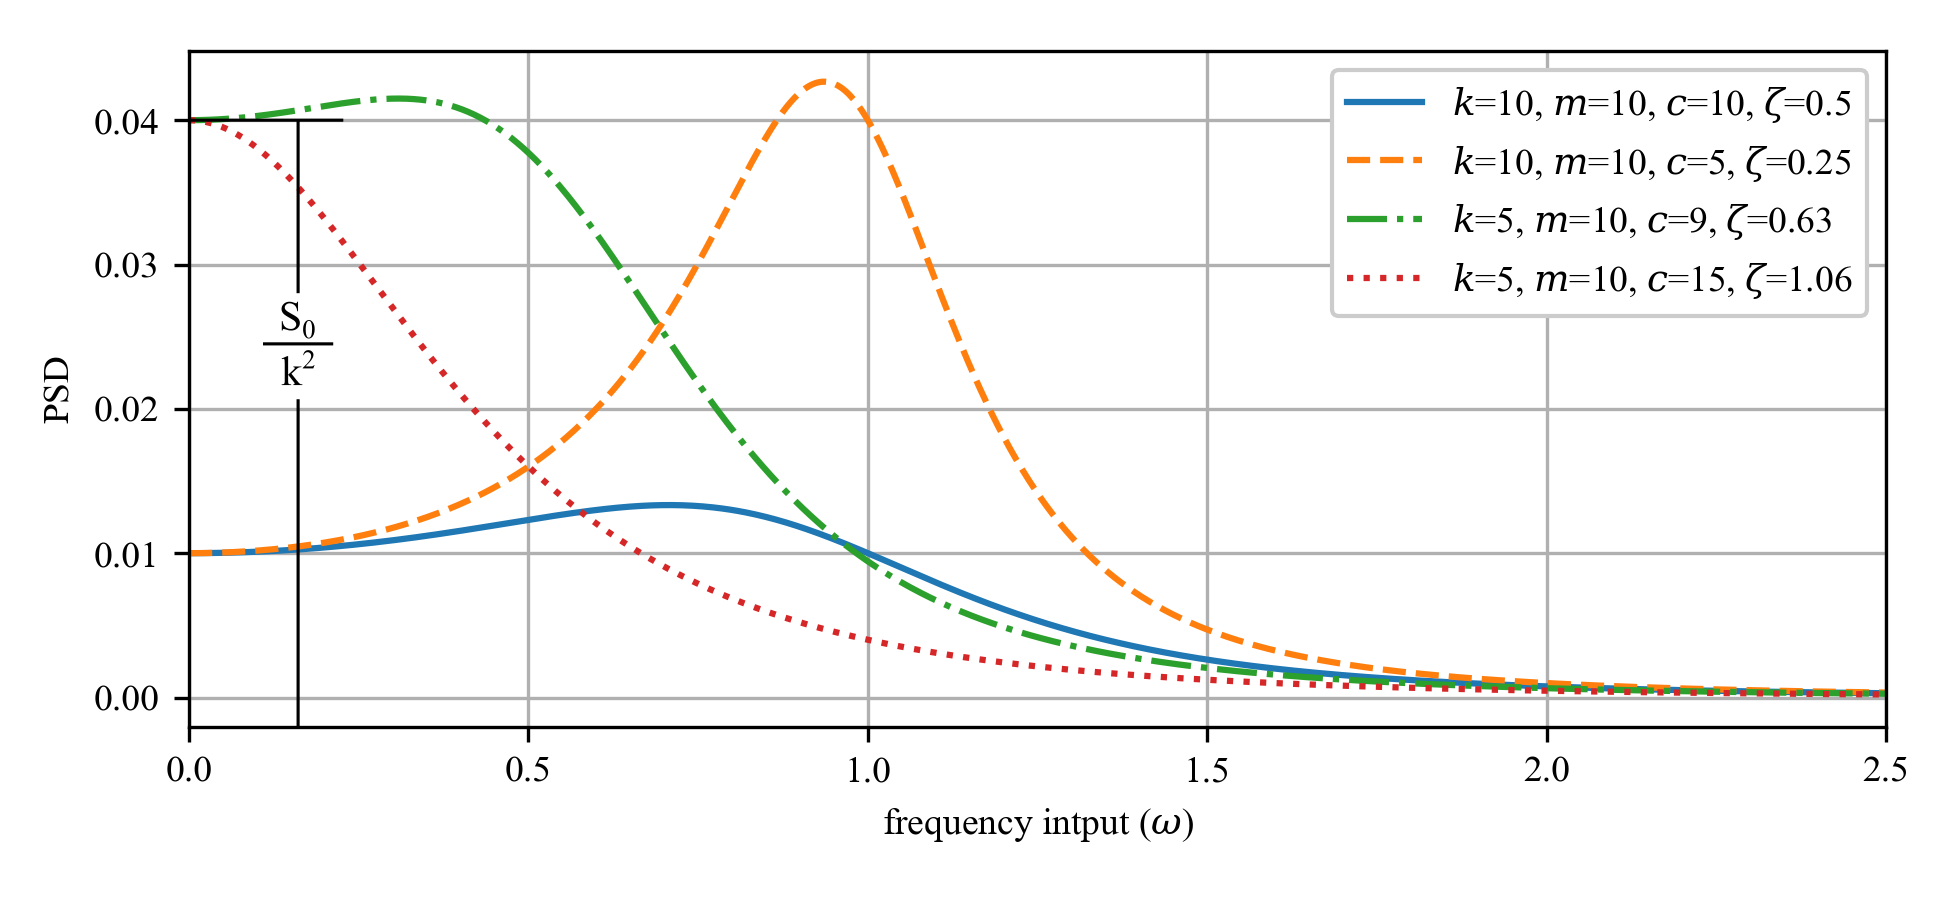
\includegraphics[width=1\textwidth]{../Figures/response_to_white_noise_with_annotation.png}
\end{figure}

\end{example}  


\begin{example}



For the same system as example 1, calculate the mean-square response of the system. 

\textbf{Solution}

Again, as the forcing function $S_{ff}(\omega)$ is constant across the frequency spectrum $S_{ff}(\omega)=S_0$ the mean-square response can be calculated as:
\begin{equation}
E[x^2] = \bar{x^2} =   S_{0} \int_{-\infty}^{\infty} |H(j\omega)|^2 d\omega
\end{equation}
Using the already tabulated response:
\begin{equation}
\int_{-\infty}^{\infty} \bigg|\frac{B_0 + j \omega B_1}{A_0+j \omega A_1 - \omega^2 A_2} \bigg|^2 d\omega = \frac{\pi (A_0 B_1^2 + A_2 B_0^2)}{A_0 A_1 A_2}
\end{equation} 
and the frequency response function:
\begin{equation}
H(j\omega) = \frac{1}{k-m\omega^2+c\omega j}
\end{equation}
when $B_0=1$, $B_1 = 0$, $A_0=k$, $A_1=c$, and $A_2 =m$. Therefore, using the tabulated expression we can show that:
\begin{equation}
E[x^2] = S_0 \frac{\pi m }{k c m} =  \frac{S_0 \pi}{k c}
\end{equation} 

\end{example}			
			
\pagebreak			
			\pagestyle{empty}
			\newgeometry{top=0.5in, bottom=0.5in,left=0.5in, right=0.5in}
			\vspace{-25ex}
			\begin{center}
			{\large{}\textbf{Table of Laplace Transforms for Vibrations}} \\
			\normalsize{} This is a partial lists of important Laplace transforms for vibrations that assumes \\ zero initial conditions, $0 < t$, and $\zeta < 1$.
			\end{center}
			
			\vspace{0ex}
			{\small
			\renewcommand{\arraystretch}{1.5}
			\begin{multicols}{2}
			\begin{center}
			\begin{tabbing}
			\hspace*{1.5 in}\=\hspace{1.5in}\= \kill
				$f(t)$ \> $\Laplace{f(t)}=F(s)$ \> \\ \noindent\rule{8.0cm}{0.4pt} \\
				$\delta(t)$	\> 1 \> \LTNUM \\ \\
				$\delta(t-t_0)$ \> $e^{-st_0}$ \>\LTNUM \\ \\
				$1$       			 \> $\dfrac{1}{s}$           \>\LTNUM \\ \\
				$e^{at}$ 	\> $\dfrac{1}{s-a}$ 	\>\LTNUM \\ \\
				$\sin (\omega t) $ 	\> $\dfrac{\omega}{s^2+\omega^2}$ \>\LTNUM \\ \\
				$\cos (\omega t) $ 	\> $\dfrac{s}{s^2+\omega^2}$ \>\LTNUM \\ \\
				
				$\sinh (\omega t) $	\> $\dfrac{\omega}{s^2-\omega^2}$ \>\LTNUM \\ \\
				$\cosh (\omega t) $	\> $\dfrac{s}{s^2-\omega^2}$ \>\LTNUM \\ \\
				$\dfrac{1}{\omega^2}\big(1-\cos(\omega t)\big)$ \> $\dfrac{1}{s(s^2+\omega^2)}$ \>\LTNUM \\ \\
				$\dfrac{1}{\omega_d}e^{-\zeta \omega t}\sin(\omega_d t)$ \> $\dfrac{1}{s^2+2\zeta \omega s+\omega^2}$ \>\LTNUM \\ \\
				$1-\dfrac{\omega}{\omega_d}e^{-\zeta \omega t}\sin(\omega_d t + \phi)$, $\phi =\cos^{-1}(\zeta) \dots $ \\ \> $\dfrac{\omega^2}{s(s^2+2\zeta \omega s+\omega^2)}$ \>\LTNUM \\ \\
				$\dfrac{t^{n-1}}{(n-1)!}$, $ n=1,2,\dots $ \> $\dfrac{1}{s^n}$ \>\LTNUM \\ \\
				$t^n $, $n=1,2,\dots$     \> $\dfrac{n!}{s^{n+1}}$    \>\LTNUM \\ \\
				$t^ne^{\omega t}$, $ n=1,2,\dots $	\> $\dfrac{n!}{(s-\omega)^{n+1}}$	\>\LTNUM \\ \\
				$\dfrac{1}{\omega}(1-e^{-\omega t}) $	\> $\dfrac{1}{s(s+\omega)}$	\>\LTNUM \\ \\
				$\dfrac{1}{\omega^2}(e^{-\omega t}+\omega t - 1) $	\> $\dfrac{1}{s^2(s+\omega)}$	\>\LTNUM \\ \\
			\end{tabbing}
			\end{center}
			
			\columnbreak
			
			\begin{center}
			\begin{tabbing}
			\hspace*{1.5in}\=\hspace{1.5in}\= \kill
				$f(t)$ \> $\Laplace{f(t)}=F(s)$ \> \\ \noindent\rule{8.0cm}{0.4pt} \\
				$\dfrac{1}{\omega^3}\big(\omega t - \sin(\omega t)\big) $	\> $\dfrac{1}{s^2(s^2+\omega^2)}$	\>\LTNUM \\ \\
				$\dfrac{1}{2\omega^3}\big(\sin(\omega t) - \omega t \cos(\omega t)\big) \dots $	\\ \> $\dfrac{1}{(s^2+\omega^2)^2}$	\>\LTNUM \\ \\
				$\dfrac{t}{2\omega} \sin(\omega t)$	 \> $\dfrac{s}{(s^2+\omega^2)^2}$	\>\LTNUM \\ \\
				$t\sin (\omega t) $  	\> $\dfrac{2\omega s}{(s^2+\omega^2)^2}$ \>\LTNUM \\ \\
				$t\cos (\omega t) $  	\> $\dfrac{s^2-\omega^2}{(s^2+\omega^2)^2}$ \>\LTNUM \\ \\
				$e^{at}\sin (\omega t) $	\> $\dfrac{\omega}{(s-a)^2+\omega^2}$  \>\LTNUM \\ \\
				$e^{at}\cos (\omega t) $	\> $\dfrac{s-a}{(s-a)^2+\omega^2}$  \>\LTNUM \\ \\
				$e^{at}\sinh (\omega t) $	\> $\dfrac{\omega}{(s-a)^2-\omega^2}$  \>\LTNUM \\ \\
				$e^{at}\cosh (\omega t) $	\> $\dfrac{s-a}{(s-a)^2-\omega^2}$  \>\LTNUM \\ \\
				$\dfrac{1}{\omega_2}\sin(\omega_2 t) - \dfrac{1}{\omega_1}\sin (\omega_1 t) \dots $	 \\ \> $\dfrac{\omega_1^2-\omega_2^2}{(s^2+\omega_1^2)(s^2+\omega_2^2)}$	\>\LTNUM \\ \\
				$\cos(\omega_2 t) - \cos (\omega_1 t)  $	\> $\dfrac{s(\omega_1^2-\omega_2^2)}{(s^2+\omega_1^2)(s^2+\omega_2^2)}$	\>\LTNUM \\ \\
				$e^{at}f(t)$	\> $F(s-a)$	\>\LTNUM \\ \\ 
				$f(t-a)\Phi(t-a)$ \> $e^{-as}F(s)$ \>\LTNUM \\ \\
				$\Phi(t-a)$ \> $\dfrac{e^{-as}}{s}$ \>\LTNUM \\ \\
				$f'(t)$ 	\> $sF(s) - f(0)$ \>\LTNUM \\ \\
			\end{tabbing}
			\end{center}
			\end{multicols}
			}
			
			% Unused Laplace Transforms
			%$f^{n}(t)$ 	\> $s^nF(s) - s^{(n-1)} f(0) - $ \\ \\
			% \> $\cdots - f^{(n-1)}(0)$ \>\LTNUM \\ \\
			%$\displaystyle{\int_0^t f(x)g(t-x)dx}$ \> $F(s)G(s)$ \>\LTNUM \\ \\
			%
			%$t^x$ ($x\geq-1\in\mathbb{R}$)     \> $\dfrac{\Gamma(x+1)}{s^{x+1}}$ \>\LTNUM\\ \\
			%
			%$\dfrac{e^{at}-e^{bt}}{a-b}$	\> $\dfrac{1}{(s-a)(s-b)}$ \>\LTNUM\\ \\ 
			%$f(t)$ \> $\Laplace{f(t)}=F(s)$ \> \\ \\
			%$\dfrac{ae^{at}-be^{bt}}{a-b}$	\> $\dfrac{s}{(s-a)(s-b)}$ \>\LTNUM\\ \\ 
			%$te^{at}$	\> $\dfrac{1}{(s-a)^2}$	\>\LTNUM \\ \\
			%$t\sinh (\omega t) $  	\> $\dfrac{2\omega s}{(s^2-\omega^2)^2}$ \>\LTNUM \\ \\
			%$t\cosh (\omega t) $  	\> $\dfrac{s^2+\omega^2}{(s^2-\omega^2)^2}$ \>\LTNUM \\ \\
			%$\dfrac{\sin (at)}{t}$	\> $\arctan \dfrac{a}{s}$ \>\LTNUM \\ \\
			%$\dfrac{1}{\sqrt{\pi t}}e^{-a^2/4t}$	\> $\dfrac{e^{-a\sqrt{s}}}{\sqrt{s}}$ \> \LTNUM \\ \\
			%$\dfrac{a}{2\sqrt{\pi t^3}}e^{-a^2/4t}$	\> $e^{-a\sqrt{s}}$ \> \LTNUM \\ \\
			%$\text{erfc}\left(\dfrac{a}{2\sqrt{t}}\right)$ \>  $\dfrac{e^{-a\sqrt{s}}}{s}$ \> \LTNUM \\ \\
			% $t^nf(t)$ 	\> $(-1)^n\dfrac{d^nF(s)}{ds^n}$  \>\LTNUM \\ \\
			%{\tiny \textcopyright  2011 B.E.Shapiro for \href{http://integral-table.com}{integral-table.com}. This work is licensed under a} \\
			
			%{\tiny\href{http://creativecommons.org/licenses/by-nc-sa/3.0/}{Creative Commons Attribution-NonCommercial-ShareAlike 3.0 Unported License}. } 
									
\end{document}


























